\section{Hiện thực hệ thống}
\subsection{Chức năng người dùng}
\subsubsection{Trang HomePage}
\indent \indent Đây là giao diện đầu tiên mà người dùng sẽ nhìn thấy khi truy cập vào hệ thống. Trang HomePage được thiết kế để cung cấp một cái nhìn tổng quan về các sự kiện trong hệ thống.
Giao diện của trang HomePage được chia thành nhiều phần khác nhau để hiển thị các danh sách sự kiện theo từng tiêu chí cụ thể.\\

\begin{figure}[H]
    \centering
    
\includegraphics[width=0.65\textwidth]{Contents/UI/USER/TrangChu.png}
    \vspace{15pt}
    \caption{Giao diện HomePage của người dùng khi chưa đăng nhập}
\end{figure}
\begin{figure}[H]
    \centering
    \includegraphics[width=0.65\textwidth]{Contents/UI/USER/TrangChu_DN.png}
    \vspace{15pt}
    \caption{Giao diện HomePage của người dùng khi đã đăng nhập}
\end{figure}
\indent \indent \textbf{Mô tả các thao tác:}
\begin{itemize}
    \item[-] \textbf{Lướt hoặc cuộn tròn:} Để xem tổng quan các sự kiện trong hệ thống với các thông tin cơ bản như tên sự kiện, poster, thời gian tổ chức và địa điểm.
    \item[-] \textbf{Sự kiện mới (Gồm tên và poster):} Nằm ở danh sách đầu tiên của trang, mỗi lần hiển thị gồm ba sự kiện và tự động chuyển sang sự kiện tiếp theo sau mỗi 3 giây. Nhấn "Nút xem chi tiết" sẽ điều hướng đến trang hiển thị chi tiết thông tin sự kiện đã chọn.
    \item[-] \textbf{Sự kiện phổ biến (Gồm tên, poster, thời gian tổ chức và địa điểm):} Nằm ở danh sách thứ hai của trang HomePage khi người dùng chưa đăng nhập hoặc danh sách thứ ba khi người dùng đã đăng nhập. Mỗi lần truy cập hoặc reload lại trang HomePage sẽ có sáu sự kiện hiện thị ngẫu nhiên. Nhân "Nút xem chi tiết" sẽ điều hướng đến trang hiển thị chi tiết thông tin sự kiện đã chọn hoặc liên kết "Xem thêm" để xem toàn bộ danh sách sự kiện thuộc mục này.
    \item[-] \textbf{Sự kiện dành cho bạn (Gồm tên, poster, thời gian tổ chức và địa điểm):} Chỉ xuất hiện ở danh sách thứ thứ hai của trang HomePage khi người dùng đã đăng nhập. Đây là danh sách chứa các sự kiện được hệ thống gợi ý giảm dần dựa trên độ phù hợp. Nhấn "Nút xem chi tiết" sẽ điều hướng đến trang hiển thị chi tiết thông tin sự kiện đã chọn hoặc liên kết "Xem thêm" để xem toàn bộ danh sách sự kiện thuộc mục này.
    \item[-] \textbf{Biểu tượng chatbot AI ở góc dưới bên phải:} Nhấn vào biểu tượng này sẽ hiển thị khung chat để người dùng có thể tương tác và nhận hỗ trợ tự động từ hệ thống.
    \item[-] \textbf{Thanh Header:} Nằm ở trên cùng của trang, các thành phần lần lượt từ trái qua phải bao gồm:
    \begin{itemize}
        \item[1.] \textbf{Logo hệ thống.}
        \item[2.] \textbf{Tên hệ thống "MyTicket":} Nhấn sẽ điều hướng về trang HomePage.
        \item[3.] \textbf{Thanh tìm kiếm:} Người dùng có thể nhập từ khóa để tìm kiếm sự kiện. Sau khi nhấn enter, hệ thống sẽ điều kiện sang trang Kết quả tìm kiếm.
        \item[4.] \textbf{Nút chức năng "Vé của tôi":} Hệ thống sẽ điều hướng đến trang tương ứng. Nếu người dùng chưa đăng nhập, hệ thống sẽ tự động hiển thị form đăng nhập yêu cầu người dùng thực hiện.
        \item[5.] \textbf{Hai nút Đăng ký và Đăng nhập (Khi chưa đăng nhập):} Khi nhấn vào nút nào, hệ thống sẽ hiển thị form tương ứng.
        \item[6.] \textbf{Avatar người dùng (Hiển thị khi đã đăng nhập và thay thế vị trí của hai nút Đăng ký và Đăng nhập):} Nhấn vào avatar sẽ hiển thị menu thả xuống với các tùy chọn "Thông tin cá nhân" và "Đăng xuất". Nếu chọn "Thông tin cá nhân" sẽ điều hướng đến trang hiển thị thông tin cá nhân của người dùng hoặc nếu chọn "Đăng xuất" sẽ đăng xuất tài khoản và điều hướng về trang HomePage.
    \end{itemize}
\end{itemize}

\subsubsection{Giao diện Chatbot AI}

\indent \indent \textbf{Các bước tương tác với ChatBot AI trong hệ thống như sau:}

\begin{itemize}
    \item[1.] \textbf{Truy cập vào biểu tượng chatbot AI:} Người dùng nhấn vào biểu tượng chatbot AI ở góc dưới bên phải của trang HomePage để mở khung chat.
    \begin{figure}[H]
        \centering
        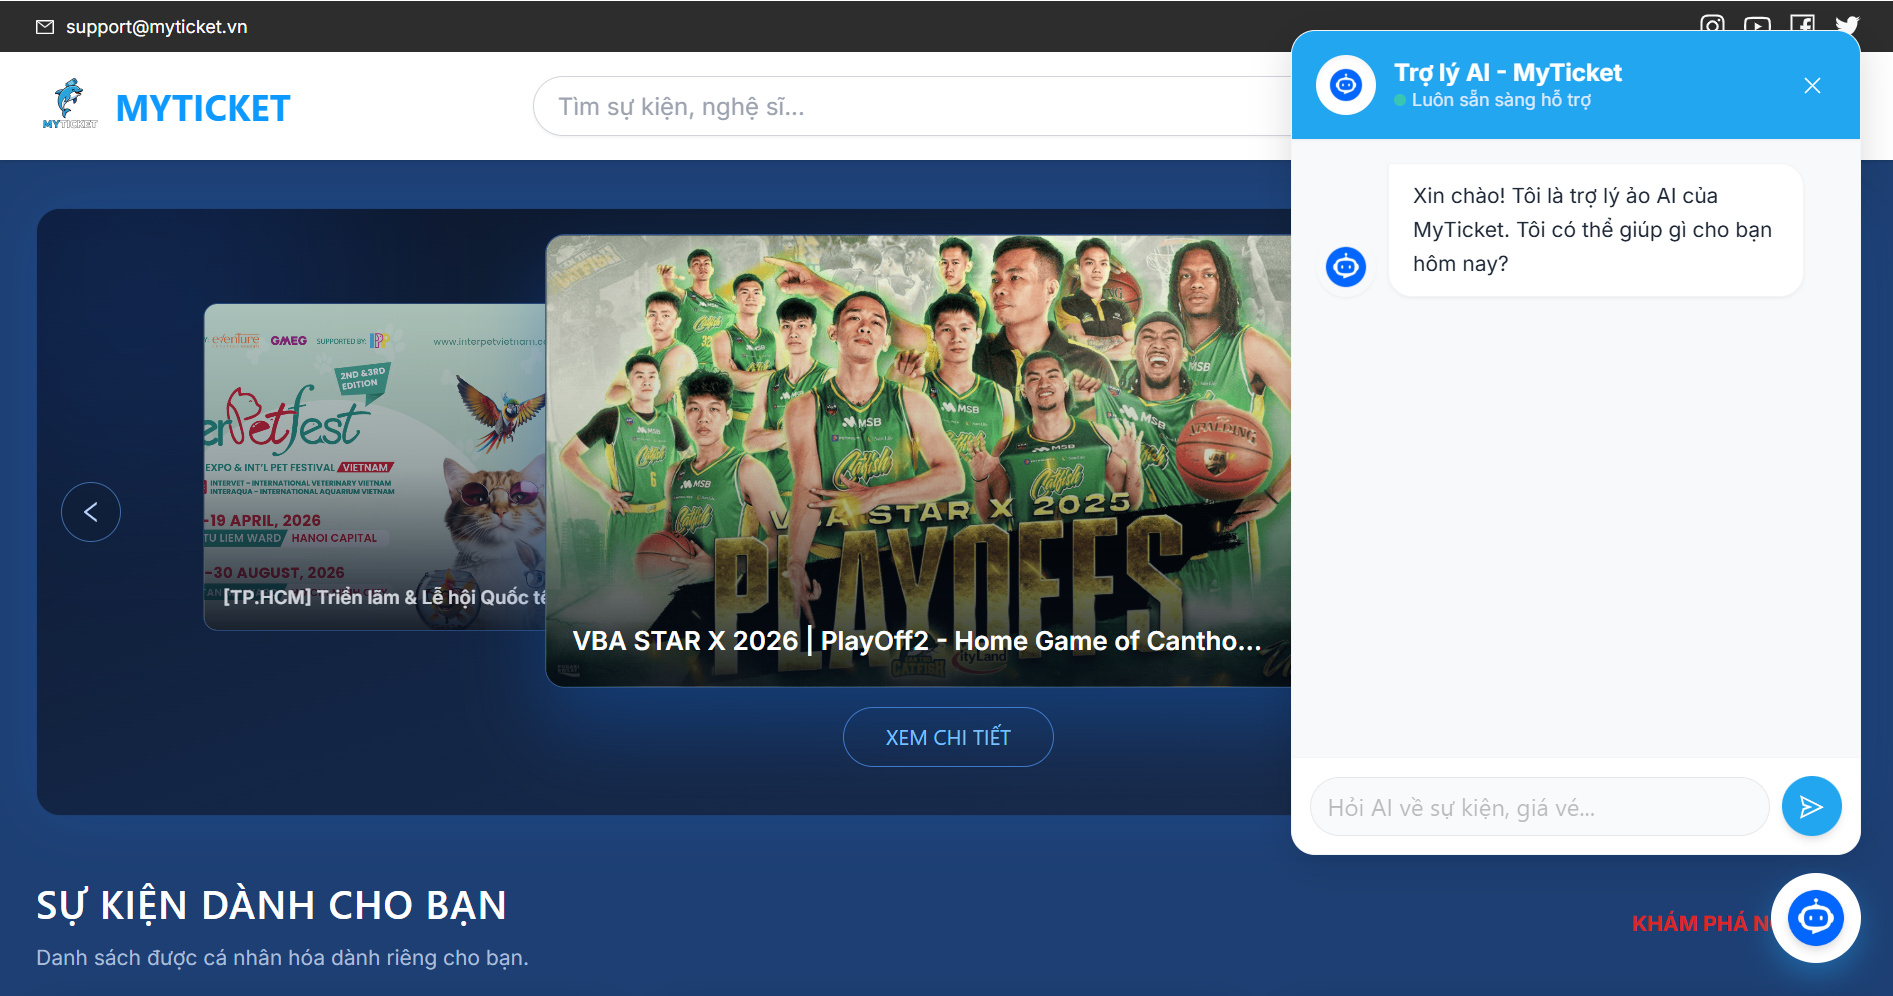
\includegraphics[width=0.65\textwidth]{Contents/UI/USER/AIChatBox.png}
        \vspace{15pt}
        \caption{Giao diện khung chat của Chatbot AI}
    \end{figure}
    
    \item[2.] \textbf{Nhập câu hỏi hoặc yêu cầu:} Người dùng có thể nhập bất kỳ câu hỏi hoặc yêu cầu nào liên quan đến việc tìm kiếm sự kiện, hỗ trợ mua vé, thông tin về sự kiện, v.v. vào khung chat. Sau đó nhấn nút Enter hoặc nút gửi để hệ thống xử lý yêu cầu.
    \begin{figure}[H]
        \centering
        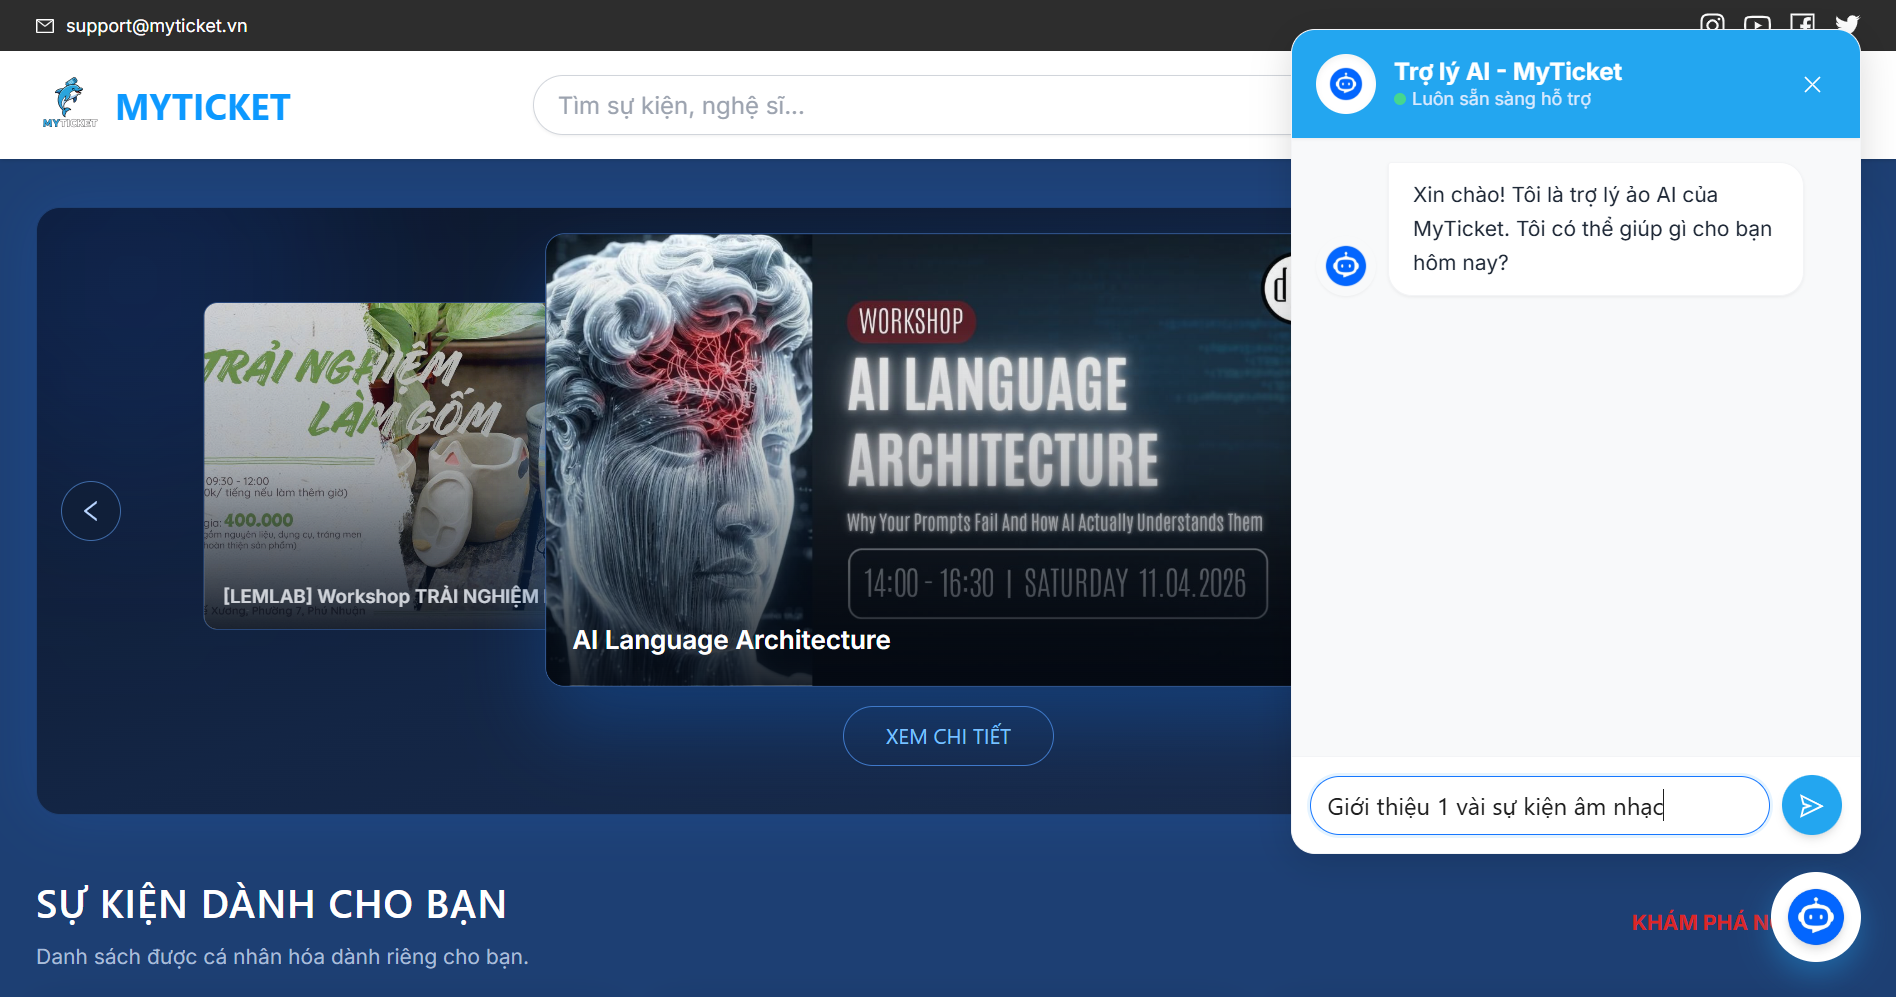
\includegraphics[width=0.65\textwidth]{Contents/UI/USER/NhapCauHoi.png}
        \vspace{15pt}
        \caption{Giao diện khung chat sau khi người dùng nhập câu hỏi}
    \end{figure}
    
    \item[3.] \textbf{Đợi phản hồi từ Chatbot AI:} Hệ thống sẽ xử lý yêu cầu của người dùng và trả về phản hồi phù hợp. Phản hồi có thể bao gồm thông tin về sự kiện, hướng dẫn mua vé, hoặc các câu trả lời liên quan khác. 
    \begin{figure}[H]
        \centering
        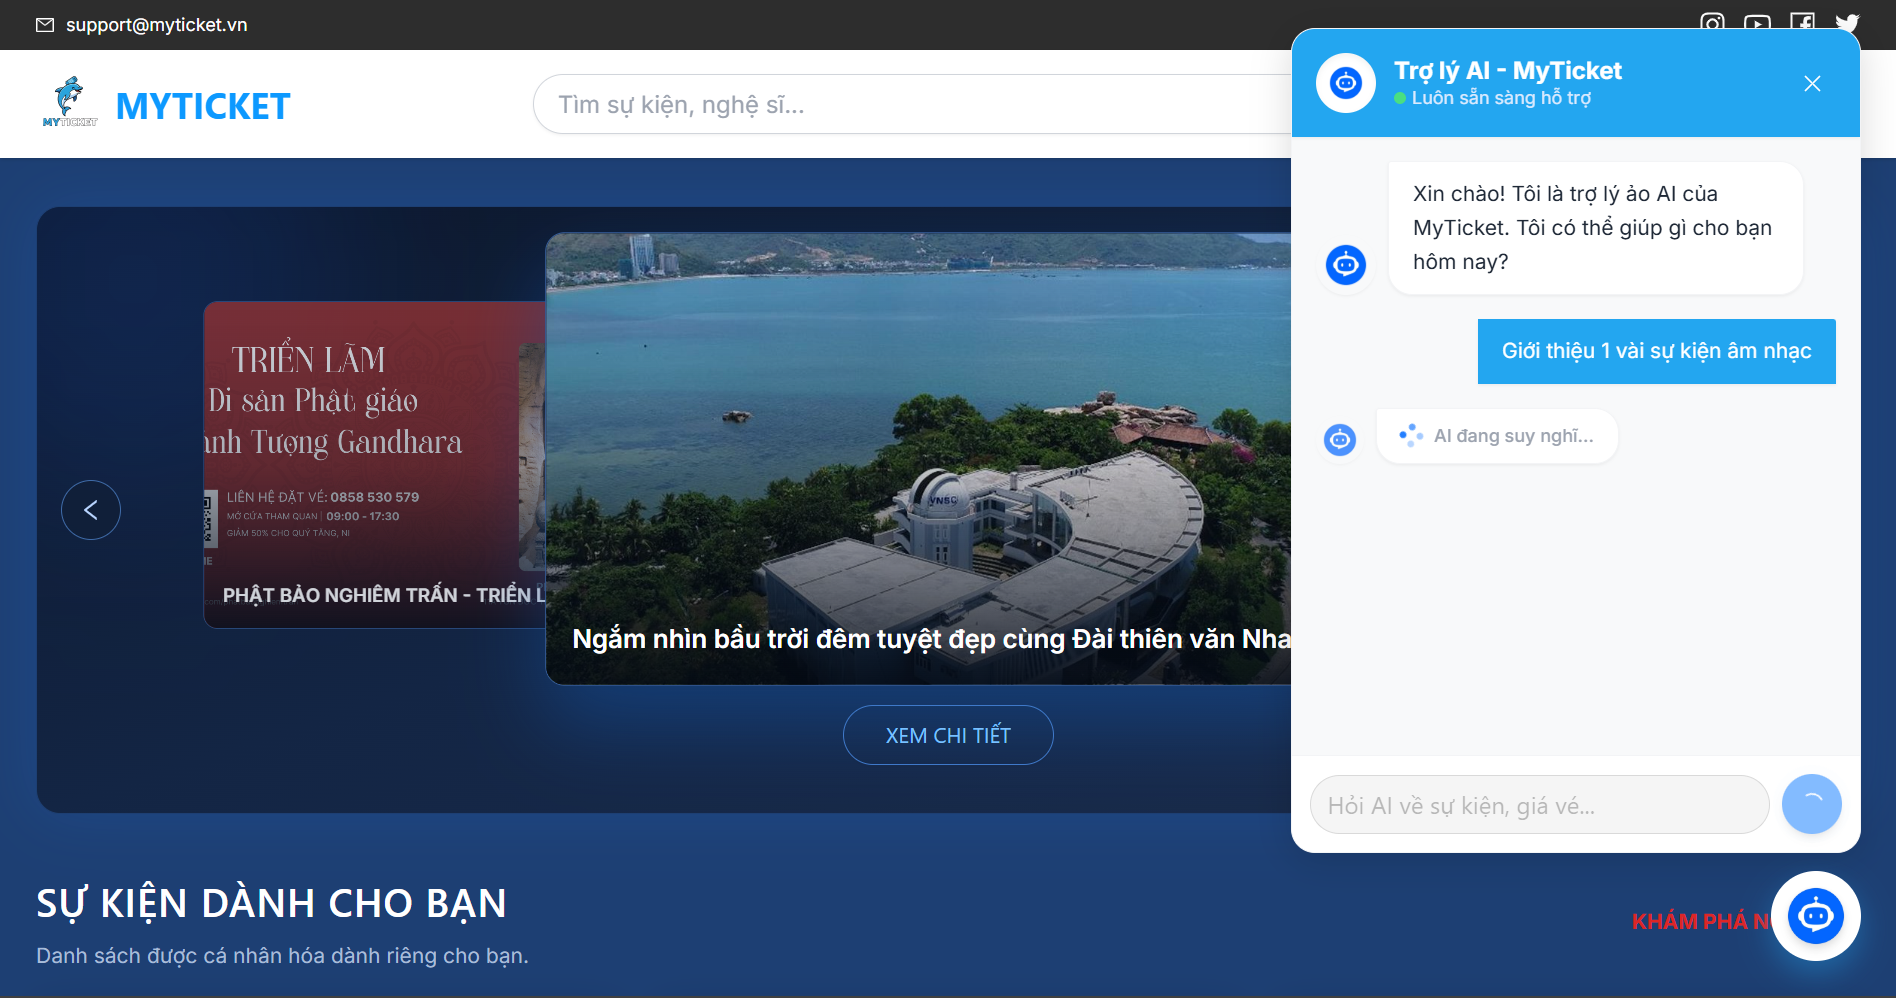
\includegraphics[width=0.65\textwidth]{Contents/UI/USER/AISuyNghi.png}
        \vspace{15pt}
        \caption{Giao diện Chatbot AI đang suy nghĩ}
    \end{figure}
    
    \item[4.] \textbf{Nhận phản hồi:} Sau khi Chatbot AI xử lý xong, người dùng sẽ nhận được phản hồi dưới dạng tin nhắn trong khung chat. Người dùng có thể tiếp tục tương tác bằng cách đặt thêm câu hỏi hoặc yêu cầu khác nếu cần bằng cách quay lại bước 1 hoặc 2.
    \begin{figure}[H]
        \centering
        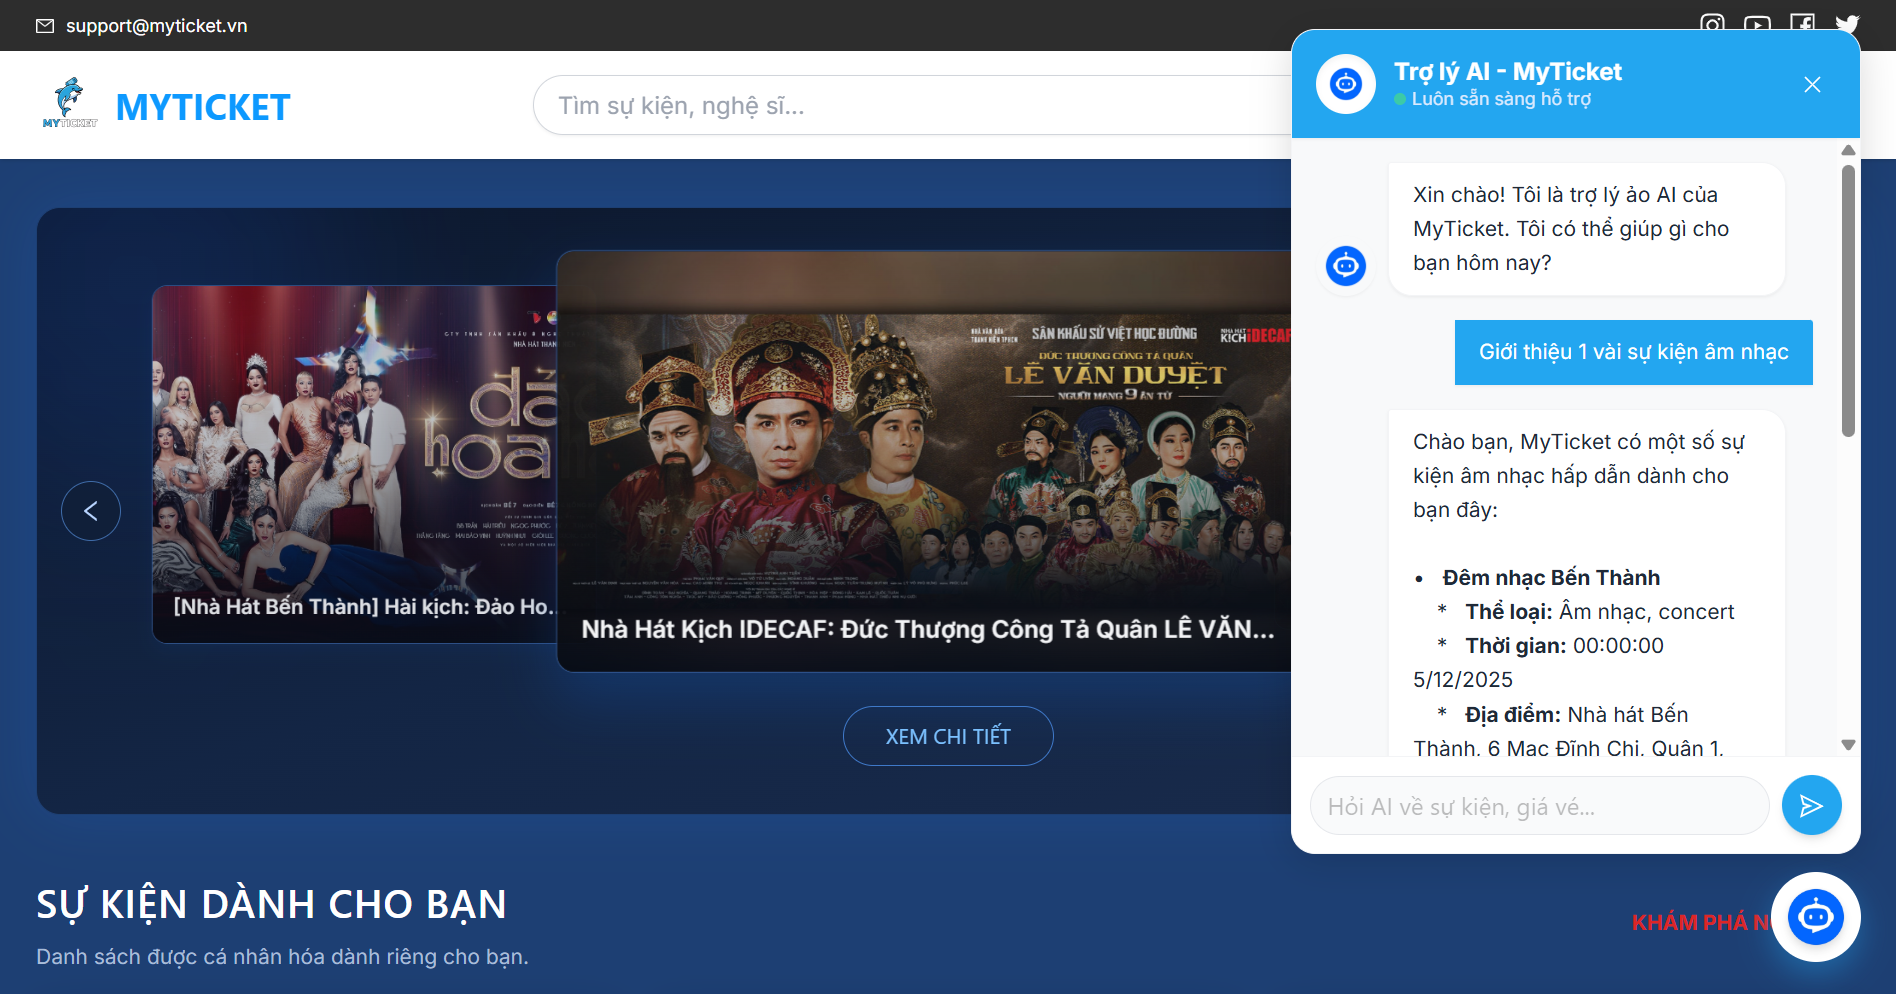
\includegraphics[width=0.65\textwidth]{Contents/UI/USER/AIPhanHoi.png}
        \vspace{15pt}
        \caption{Giao diện Chatbot AI trả về phản hồi cho người dùng}
    \end{figure}

    \item[5.] \textbf{Tắt khung chat:} Khi người dùng hoàn tất việc tương tác với Chatbot AI, họ có thể nhấn vào biểu tượng "X" ở góc trên bên phải của khung chat để đóng nó lại. Nội dung cuộc trò chuyện chỉ mất khi người dùng reload lại trang hiện tại hoặc chuyển qua trang mới. Nếu không thì khi ấn lại vào biểu tượng chatbot AI, khung chat sẽ được mở lại với nội dung cuộc trò chuyện trước đó vẫn được giữ nguyên.
\end{itemize}


\subsubsection{Tìm kiếm sự kiện}
\begin{figure}[H]
    \centering
    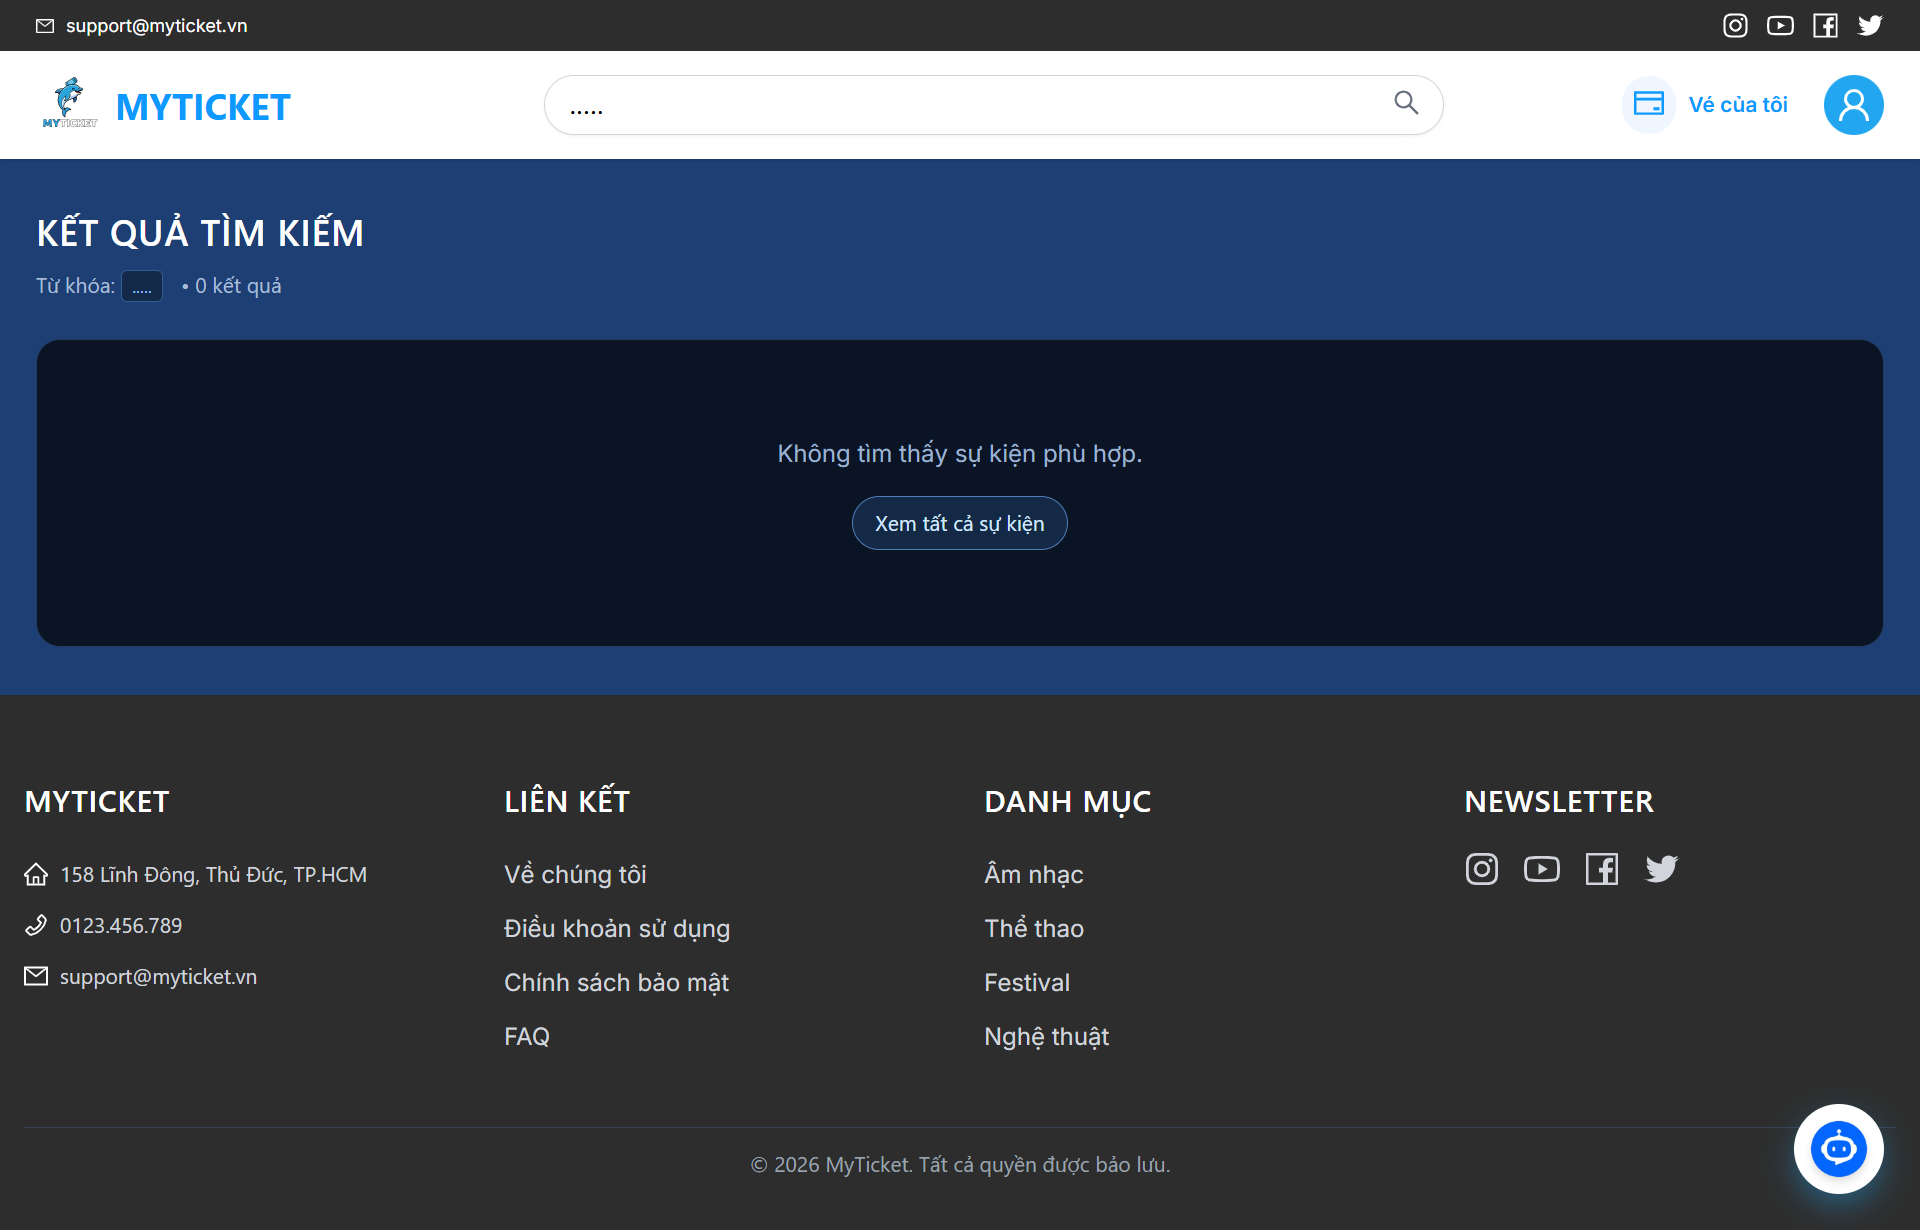
\includegraphics[width=0.65\textwidth]{Contents/UI/USER/Search without result.png}
    \vspace{15pt}
    \caption{Trang kết quả tìm kiếm khi không có sự kiện phù hợp}
\end{figure}

\begin{figure}[H]
    \centering
    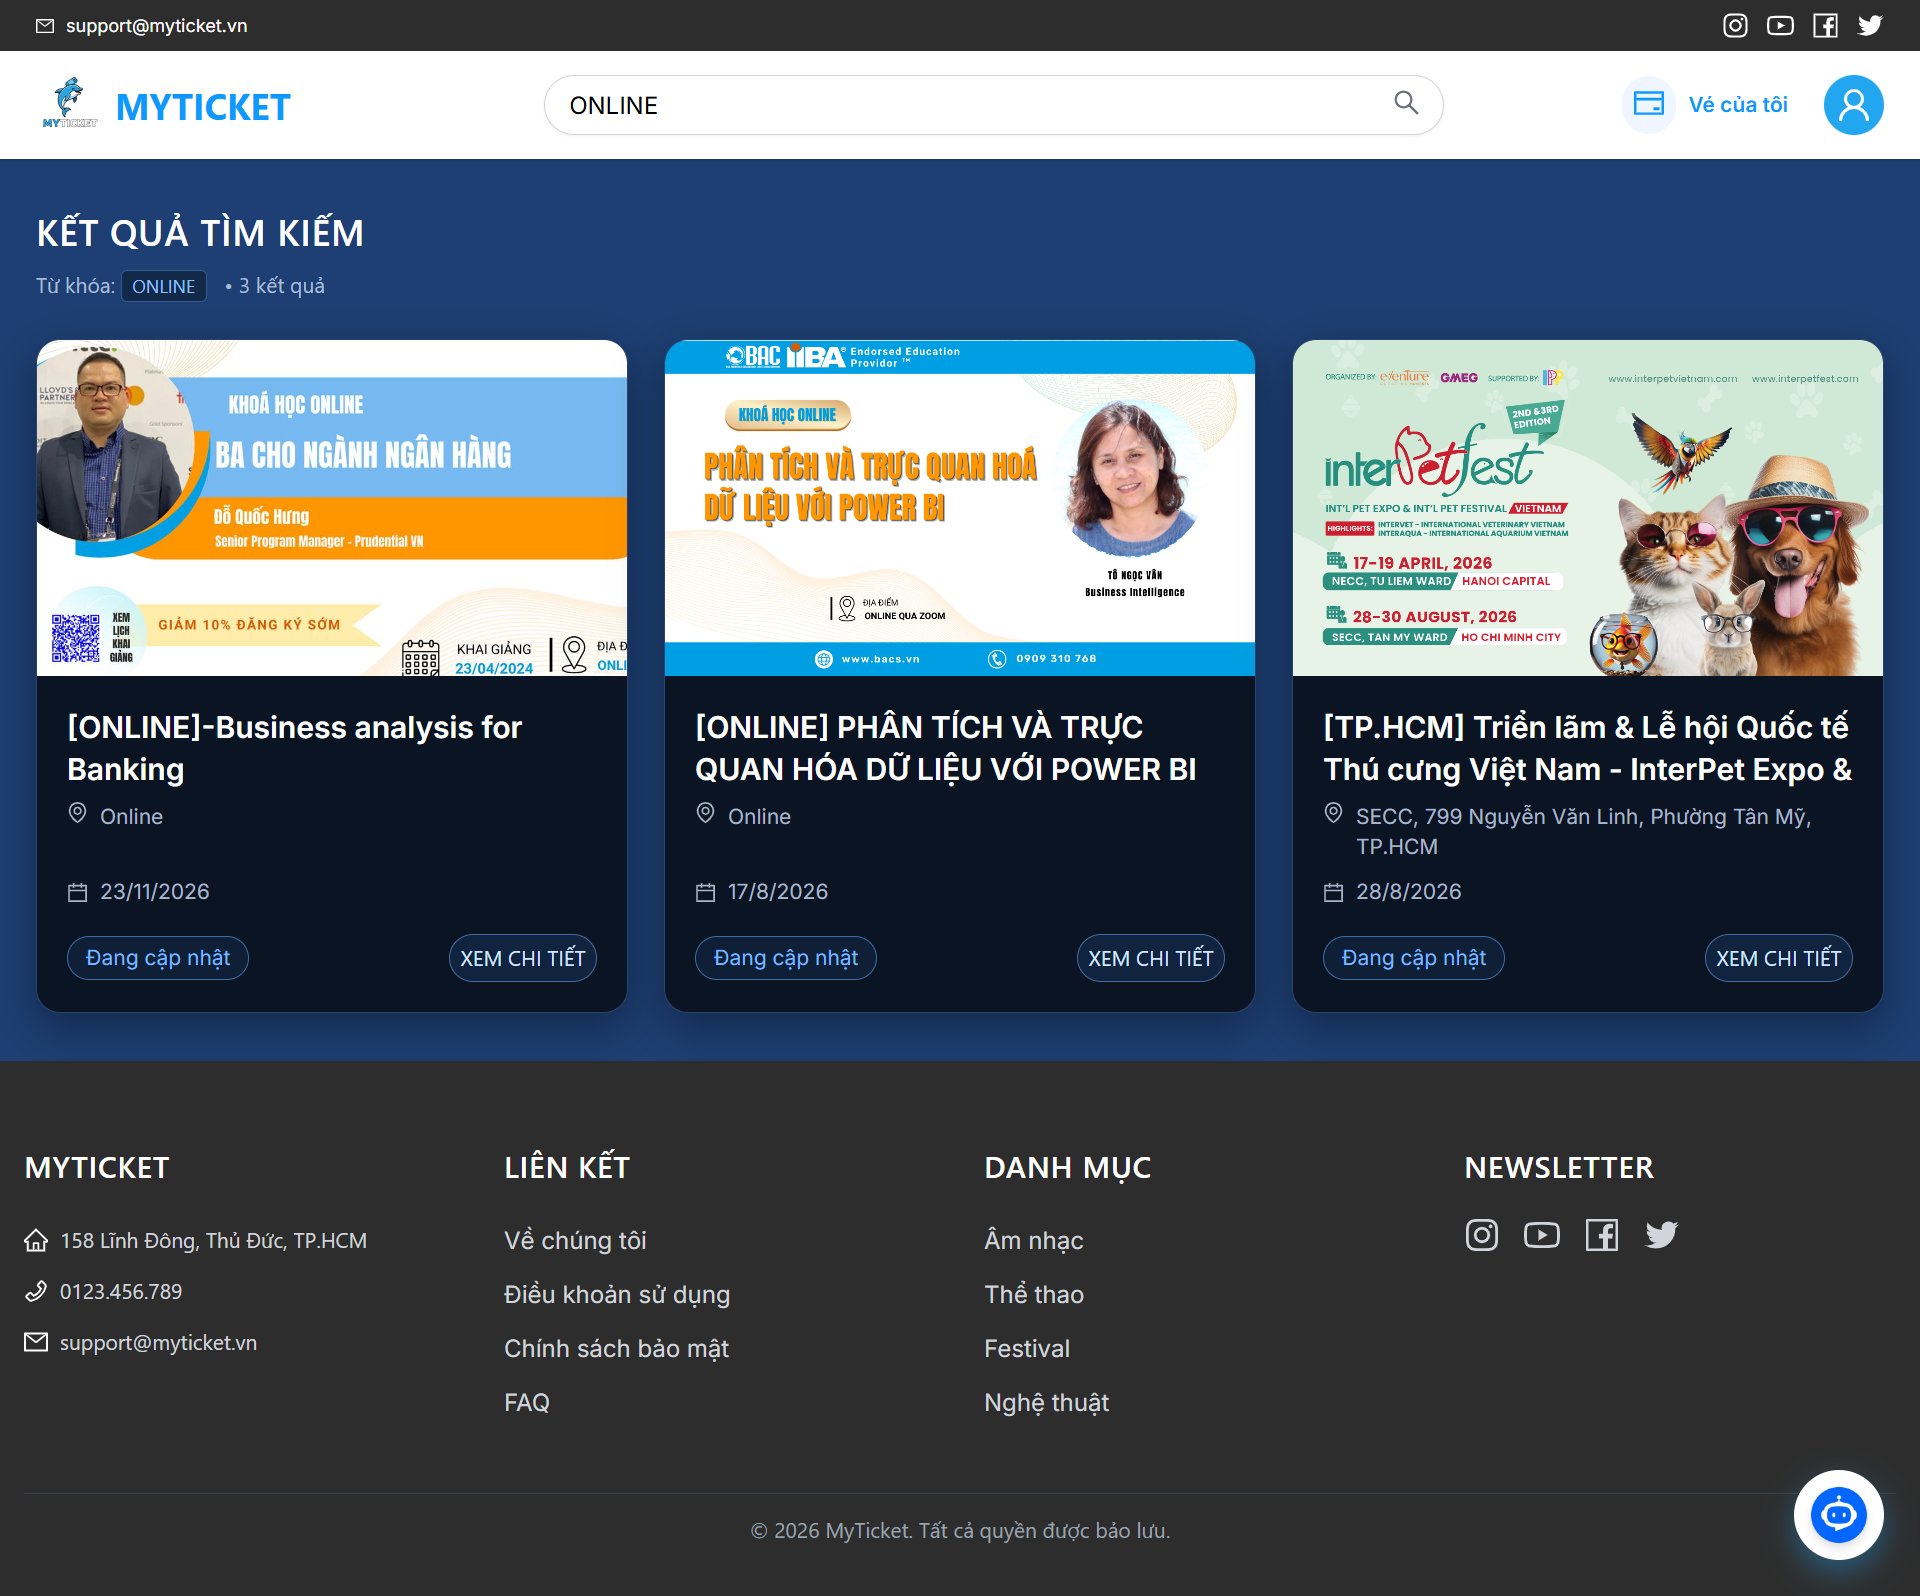
\includegraphics[width=0.65\textwidth]{Contents/UI/USER/Search with result.png}
    \vspace{15pt}
    \caption{Trang kết quả tìm kiếm khi có sự kiện phù hợp}
\end{figure}

\indent \indent \textbf{Mô tả:}\\
\indent - Khi người dùng nhập từ khóa vào thanh tìm kiếm, hệ thống sẽ truy vấn và trả về các kết quả liên quan: Danh sách sự kiện phù hợp hoặc thông báo không có kết quả phù hợp.\\
\indent - Trường hợp không có kết quả phù hợp, người dùng có thể chọn xem tất cả sự kiện đang có bằng cách nhấn vào nút ở hình.
\begin{figure}[H]
    \centering
    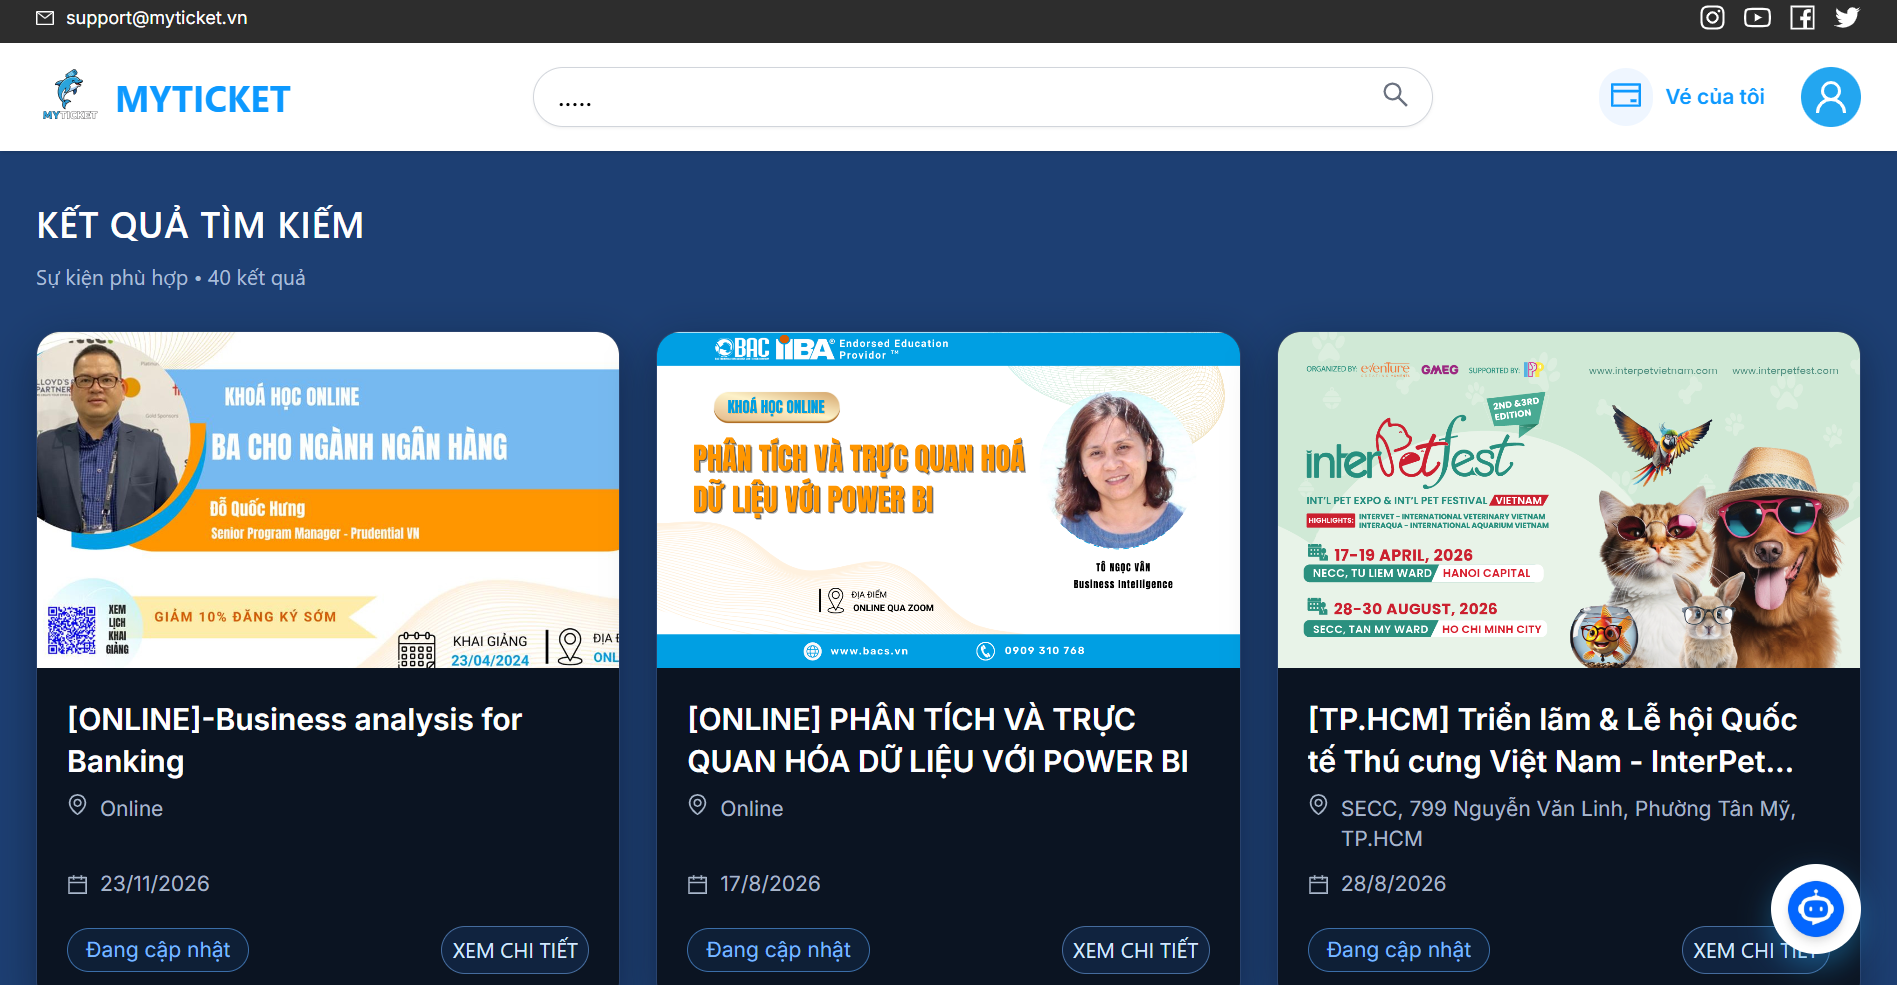
\includegraphics[width=0.65\textwidth]{Contents/UI/USER/ViewAllEvent.png}
    \vspace{15pt}
    \caption{Trang hiển thị tất cả sự kiện khi không có kết quả tìm kiếm phù hợp}
\end{figure}

\subsubsection{Giao diện Đăng nhập/Đăng ký tài khoản}

\begin{figure}[H]
    \centering
    
\includegraphics[width=0.65\textwidth]{Contents/UI/USER/ĐN.png}
    \vspace{15pt}
    \caption{Giao diện đăng nhập tài khoản}
\end{figure}

\begin{figure}[H]
    \centering
    
\includegraphics[width=0.65\textwidth]{Contents/UI/USER/Đăng ký.png}
    \vspace{15pt}
    \caption{Giao diện đăng ký tài khoản}
\end{figure}

\indent \indent - \textbf{Cách truy cập form đăng nhập hoặc đăng ký:}\\
\indent \textbf{Đăng nhập:}
\begin{itemize}
    \item[1.] Chủ động nhấn vào nút "Đăng nhập" ở thanh header khi chưa đăng nhập.
    \item[2.] Nhấn vào liên kết "Đăng nhập" ở form đăng ký tài khoản.
    \item[3.] Hệ thống tự động điều hướng đến form đăng nhập để người dùng đăng nhập lại khi đăng ký tạo tài khoản thành công.
\end{itemize} 

\indent \textbf{Đăng ký:}
\begin{itemize}
    \item[1.] Chủ động nhấn vào nút "Đăng ký" ở thanh header khi chưa đăng nhập.
    \item[2.] Nhấn vào liên kết "Đăng ký" ở form đăng nhập tài khoản.
\end{itemize}


\indent \indent - \textbf{Mô tả thao tác đăng nhập hoặc đăng ký:} Cả hai form đăng nhập và đăng ký tài khoản đều yêu cầu người dùng phải điền đầy đủ thông tin ở các trường theo đúng format quy định để có thể đăng nhập hoặc đăng ký thành công. \\
\indent \textbf{Trường hợp nhập sai thông tin yêu cầu:} Nếu có bất kỳ lỗi nào trong quá trình điền thông tin, hệ thống sẽ hiển thị thông báo lỗi tương ứng để người dùng điều chỉnh như các hình dưới đây.
\begin{itemize}
    \item[1.] \textbf{Đối với form đăng nhập}
    
    \begin{figure}[H]
        \centering
        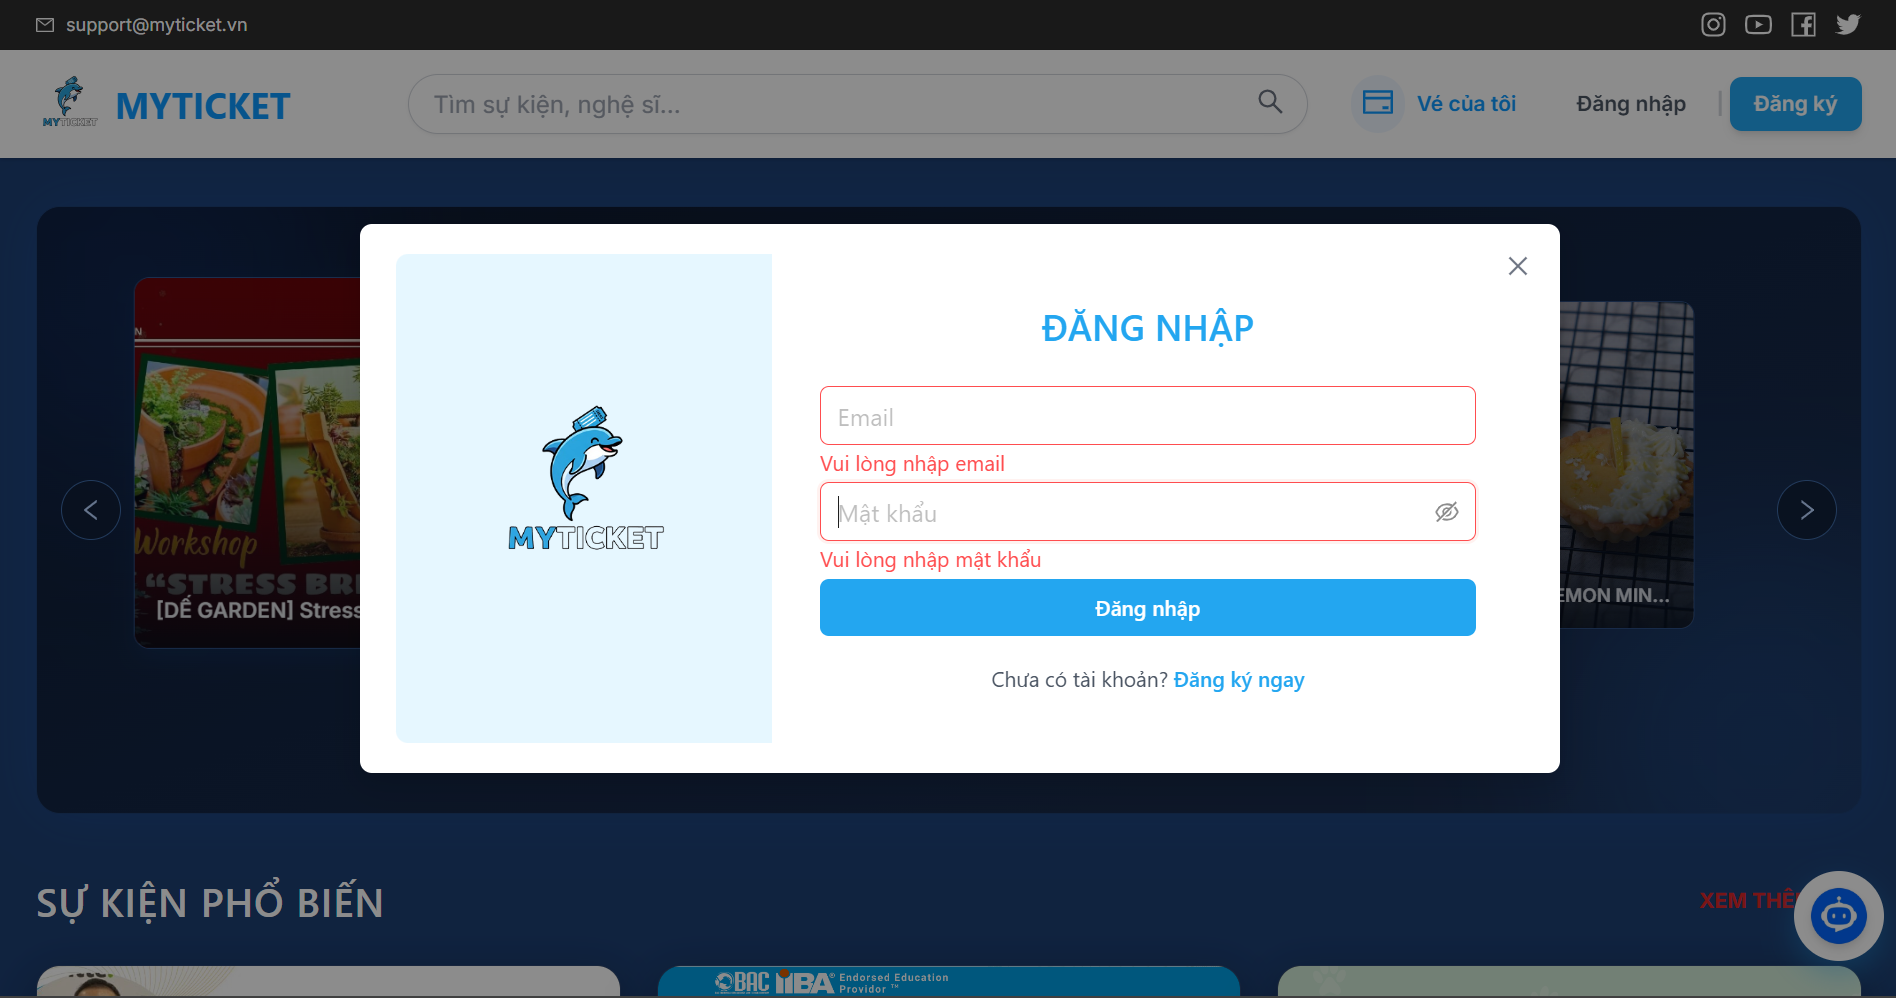
\includegraphics[width=0.65\textwidth]{Contents/UI/USER/Thiếu MK và Email ĐN.png}
        \vspace{15pt}
        \caption{Thông báo lỗi khi người dùng không nhập đủ email hoặc mật khẩu}
    \end{figure}

    \begin{figure}[H]
        \centering
        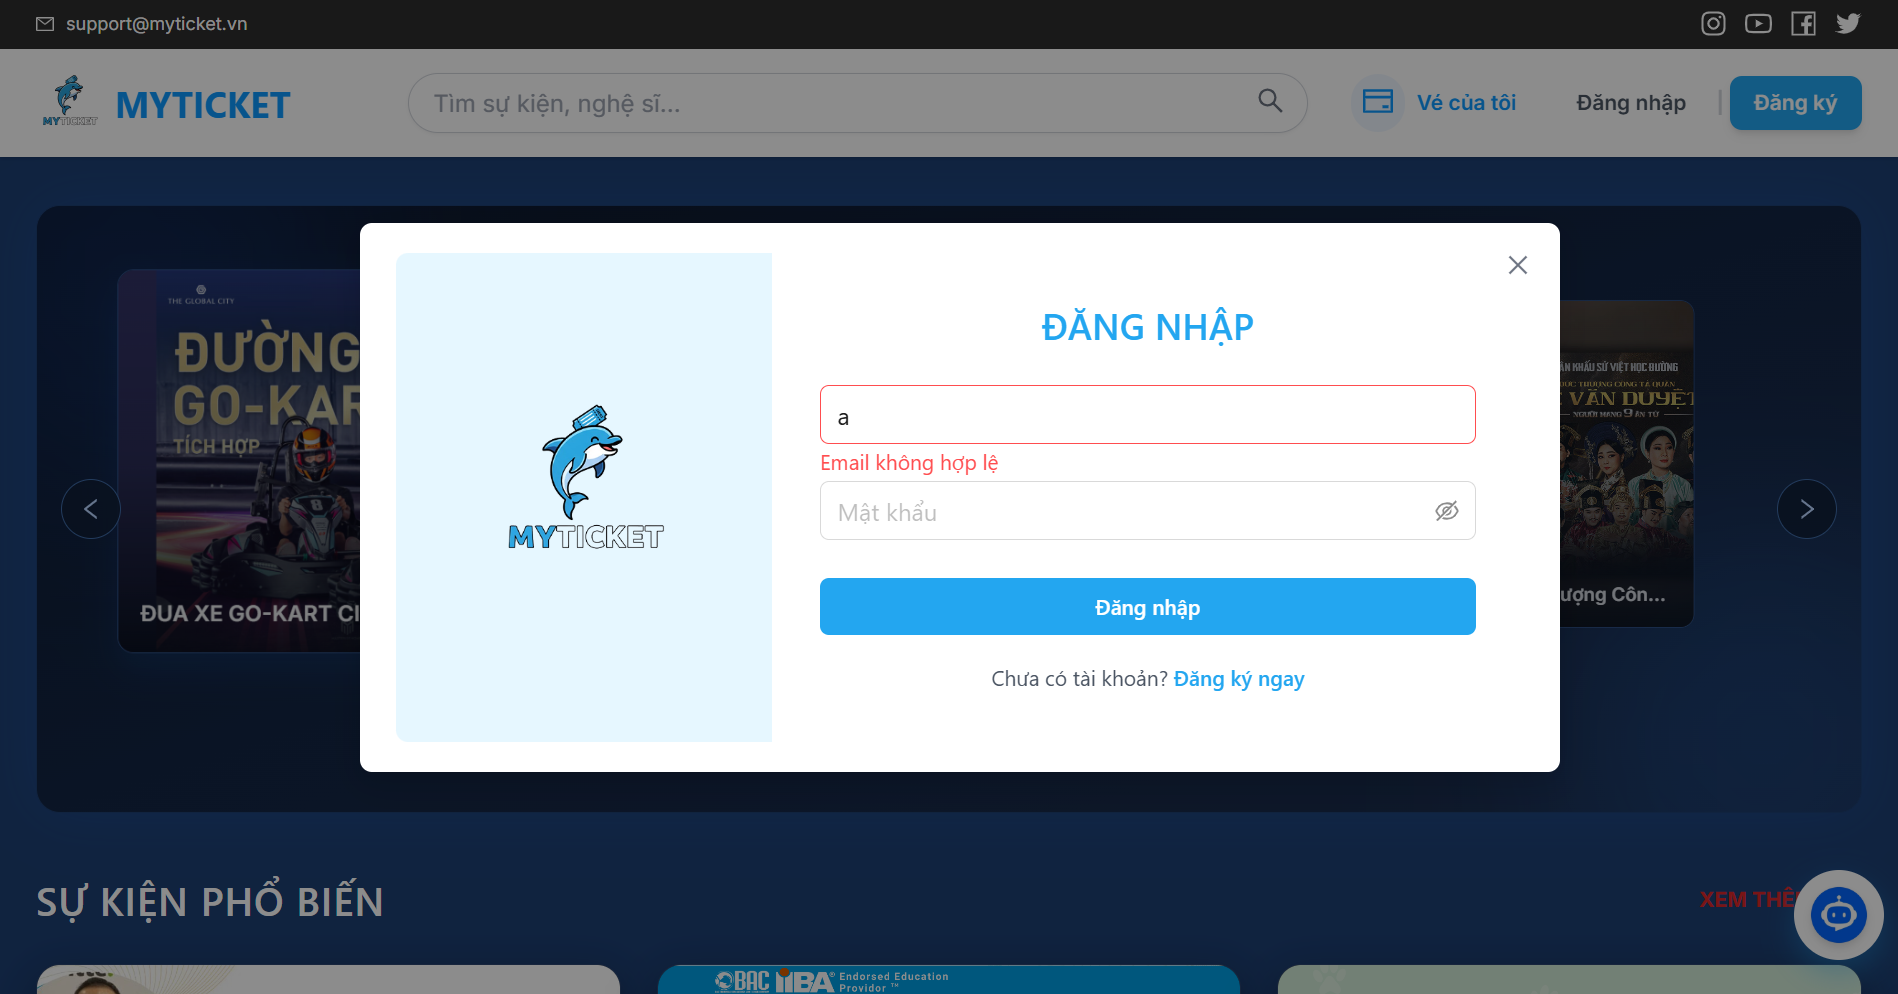
\includegraphics[width=0.65\textwidth]{Contents/UI/USER/invalid email.png}
        \vspace{15pt}
        \caption{Thông báo lỗi khi người dùng nhập email không hợp lệ}
    \end{figure}

    \begin{figure}[H]
        \centering
        
\includegraphics[width=0.65\textwidth]{Contents/UI/USER/Sai MK.png}
        \vspace{15pt}
        \caption{Thông báo lỗi khi người dùng nhập mật khẩu không hợp lệ}
    \end{figure}

    \item[2.] \textbf{Đối với form đăng ký}
    
    \begin{figure}[H]
        \centering
        
\includegraphics[width=0.65\textwidth]{Contents/UI/USER/Thieu TT ĐK.png}
        \vspace{15pt}
        \caption{Thông báo lỗi khi người dùng không nhập đủ các thông tin yêu cầu}
    \end{figure}

    \begin{figure}[H]
        \centering
        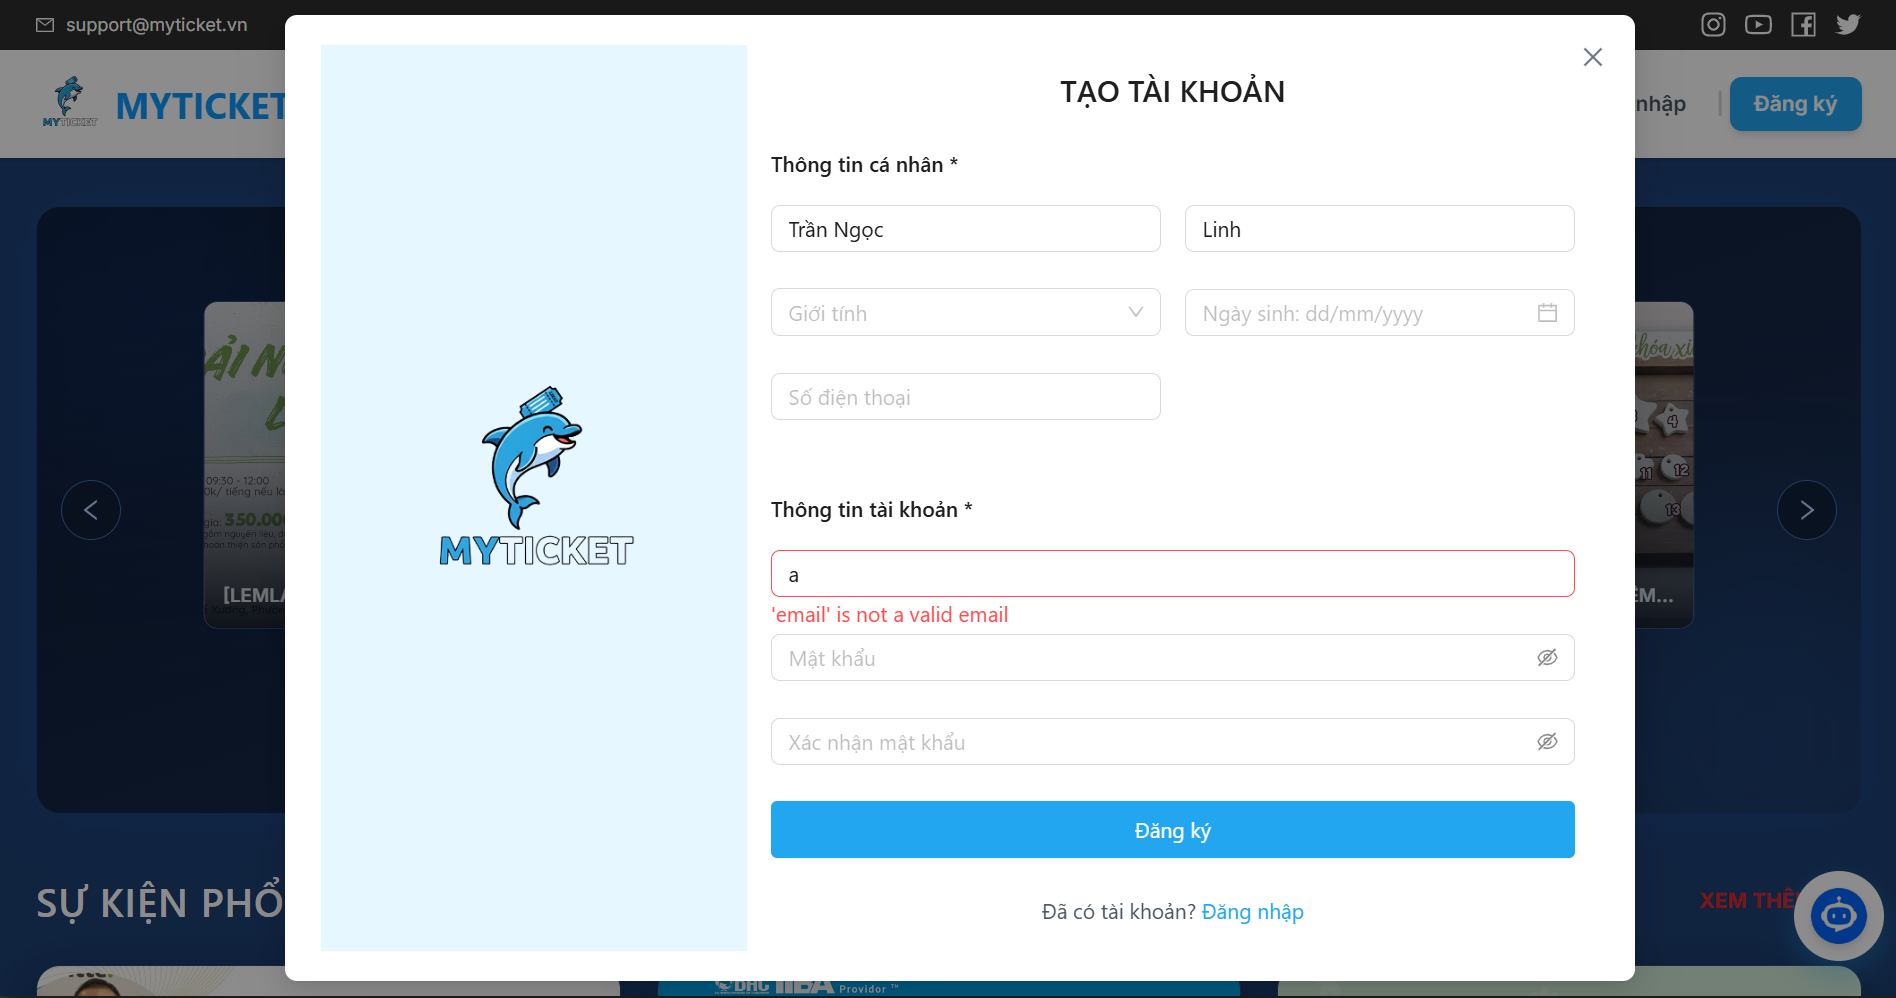
\includegraphics[width=0.65\textwidth]{Contents/UI/USER/invalid email ĐK.png}
        \vspace{15pt}
        \caption{Thông báo lỗi khi người dùng nhập email không hợp lệ}
    \end{figure}

    \begin{figure}[H]
        \centering
        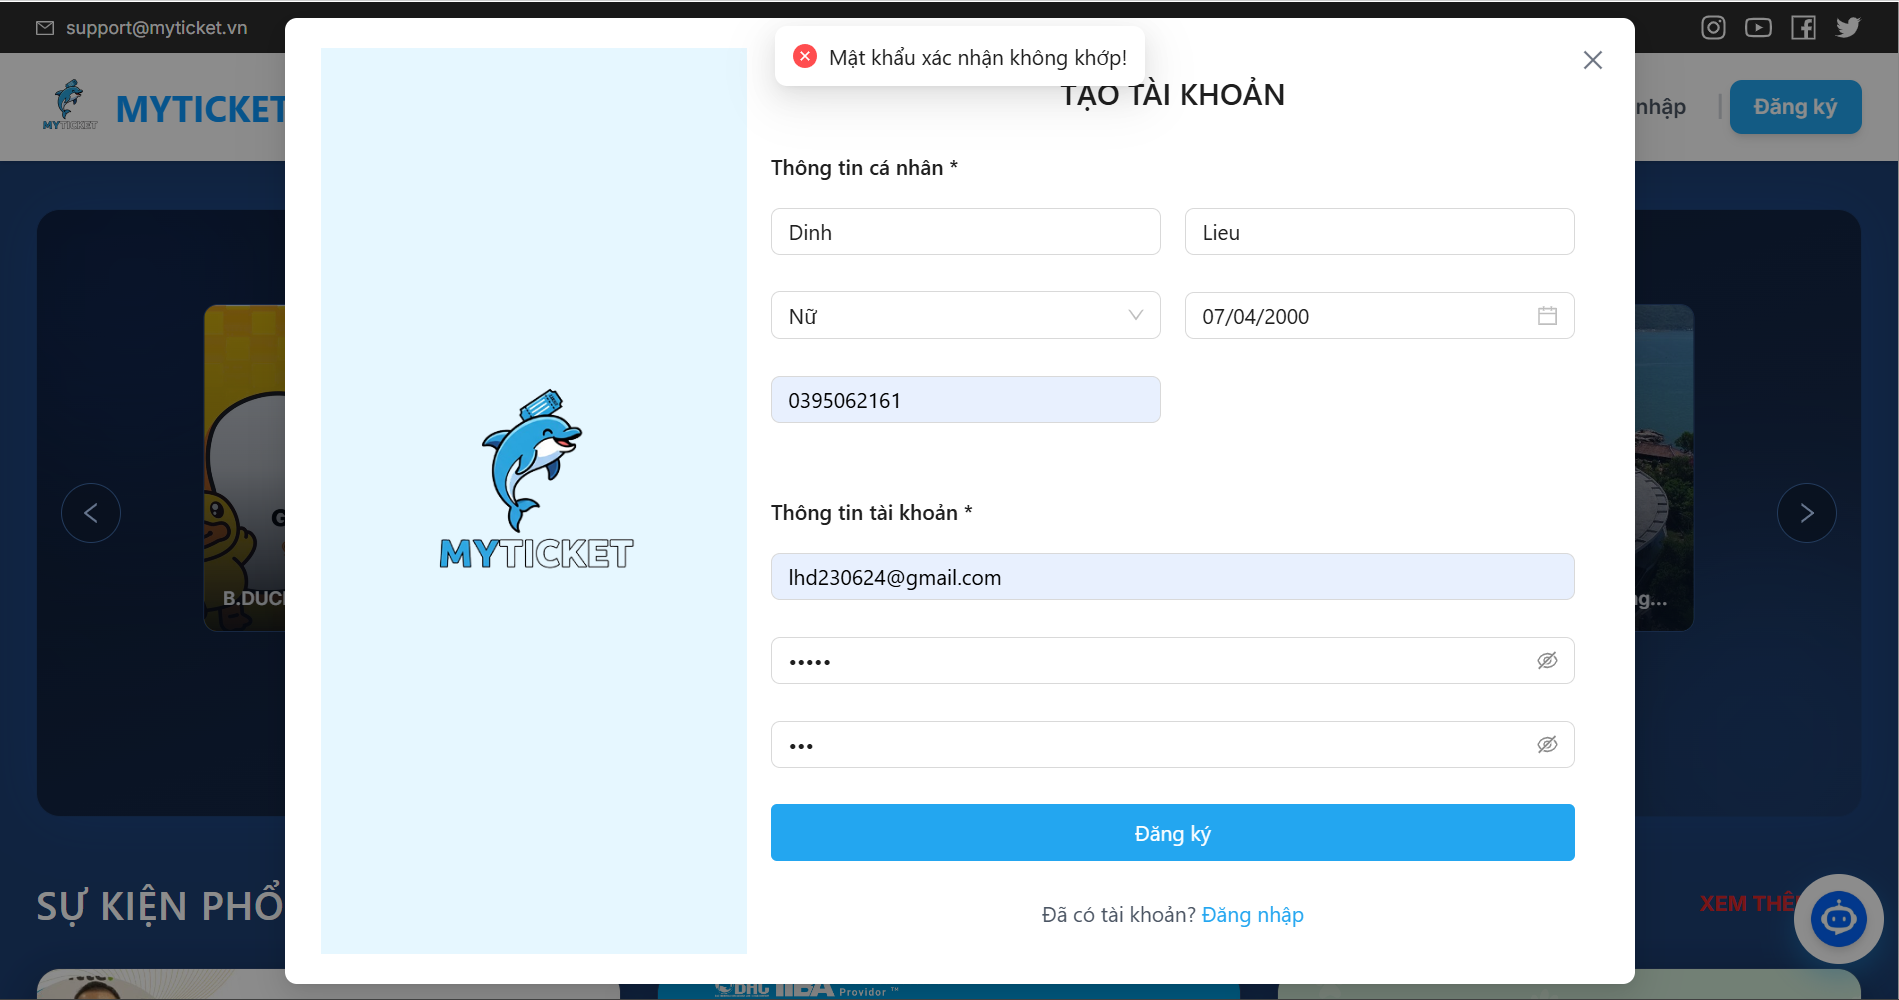
\includegraphics[width=0.65\textwidth]{Contents/UI/USER/Sai XT MK ĐK.png}
        \vspace{15pt}
        \caption{Thông báo lỗi khi người dùng nhập mật khẩu và xác nhận mật khẩu không khớp nhau}
    \end{figure}

\end{itemize}


\indent \textbf{Trường hợp nhập đúng thông tin yêu cầu:} Cả form đăng nhập và đăng ký tài khoản đều sẽ hiển thị một pop up thông báo thành công khi người dùng điền đúng thông tin yêu cầu. Sau đó, hệ thống sẽ tự động điều hướng người dùng đến trang phù hợp tùy vào role người dùng nếu đăng nhập thành công hoặc form đăng nhập nếu đăng ký thành công.

\begin{figure}[H]
    \centering
    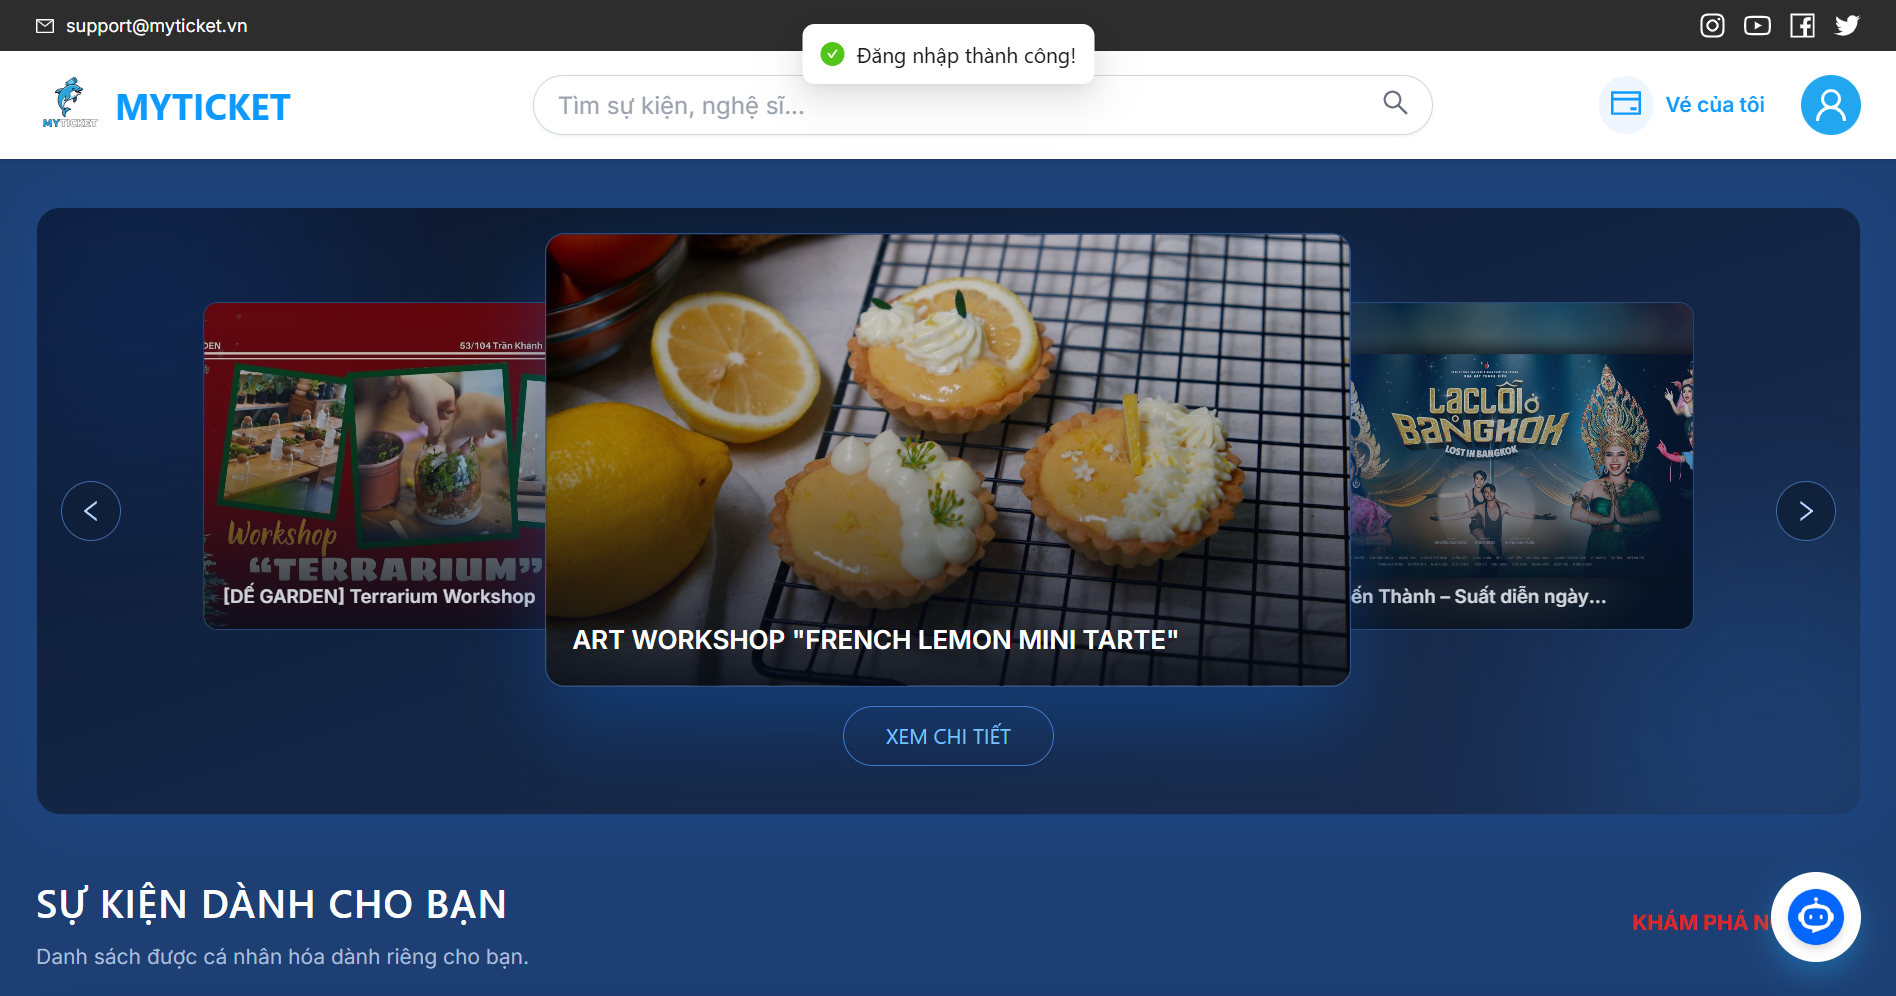
\includegraphics[width=0.65\textwidth]{Contents/UI/USER/Đăng nhập thành công.png}
    \vspace{15pt}
    \caption{Thông báo thành công khi người dùng đăng nhập thành công}
\end{figure}

\begin{figure}[H]
    \centering
    
\includegraphics[width=0.65\textwidth]{Contents/UI/USER/ĐK TC.png}
    \vspace{15pt}
    \caption{Thông báo thành công khi người dùng đăng ký tài khoản thành công}
\end{figure}

% \begin{figure}[H]
%     \centering
%     \begin{subfigure}{0.48\textwidth}
%         \centering
%         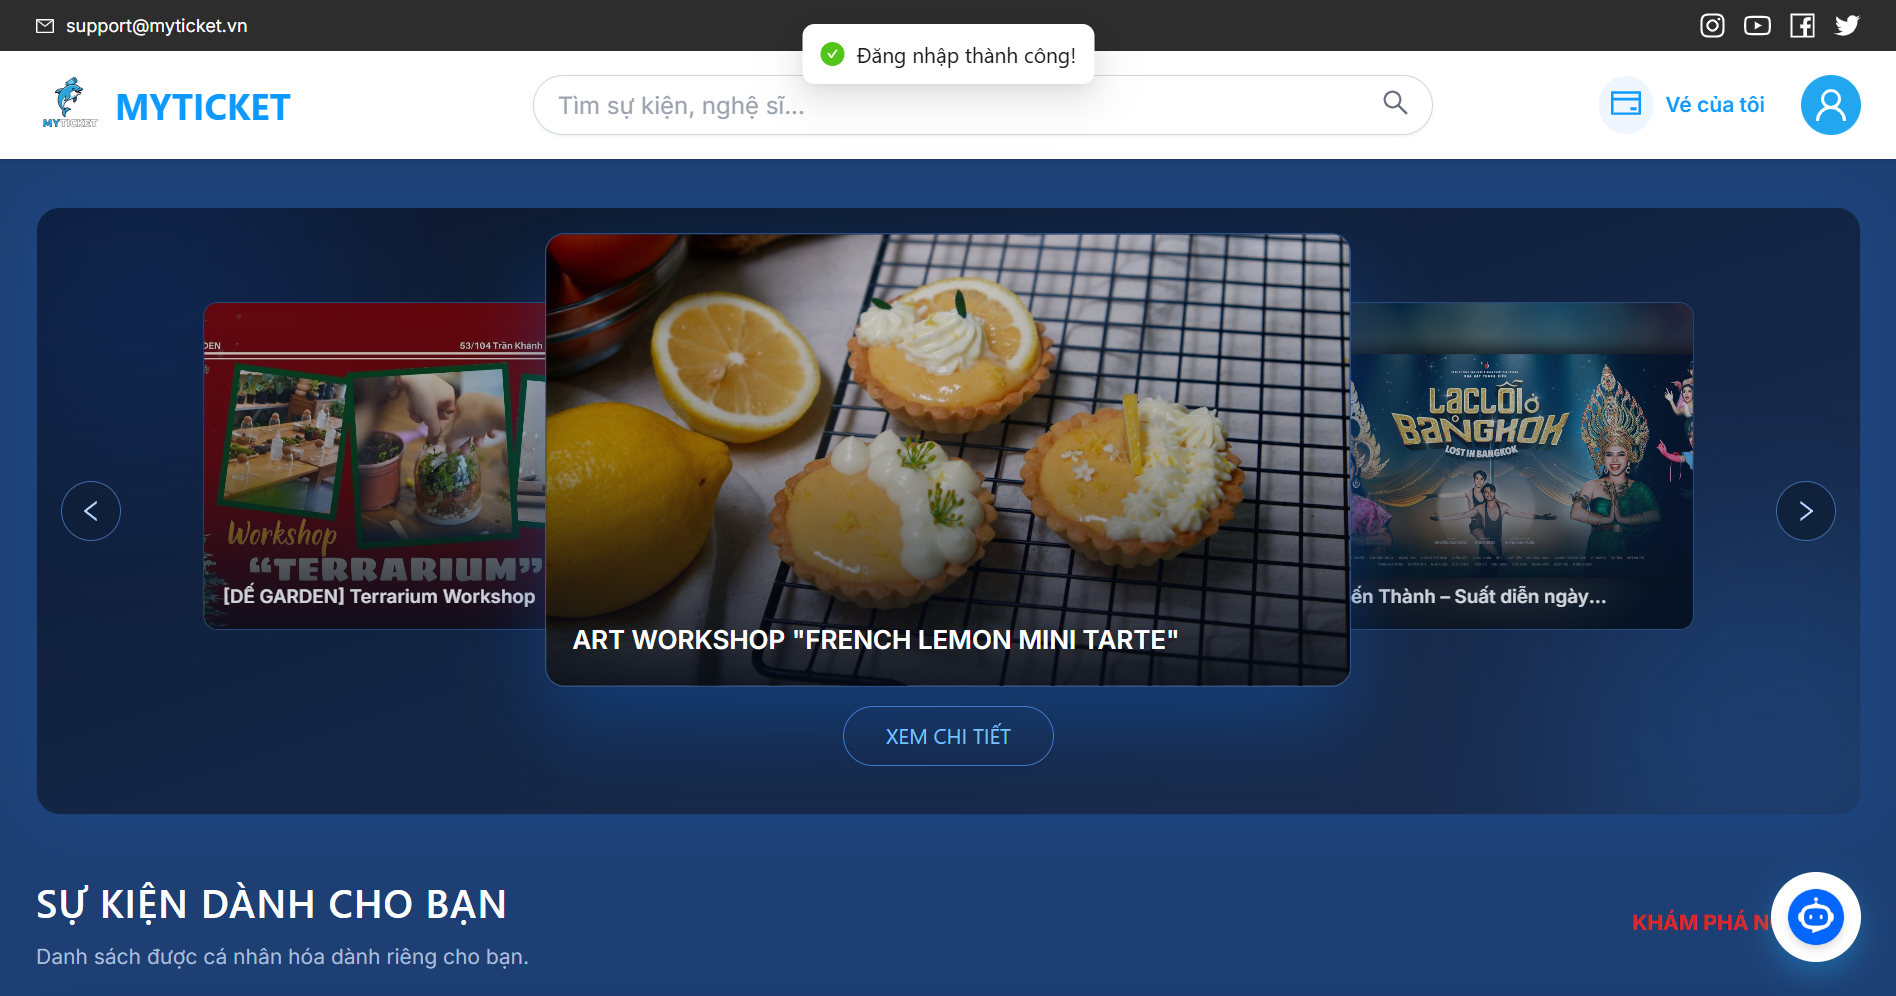
\includegraphics[width=\textwidth]{Contents/UI/USER/Đăng nhập thành công.png}
%         \caption{Đăng nhập thành công}
%     \end{subfigure}
%     \hfill
%     \begin{subfigure}{0.48\textwidth}
%         \centering
%         
\includegraphics[width=\textwidth]{Contents/UI/USER/ĐK TC.png}
%         \caption{Đăng ký tài khoản thành công}
%     \end{subfigure}

%     \vspace{10pt}
%     \caption{Thông báo hệ thống khi người dùng đăng nhập và đăng ký}
% \end{figure}

\subsubsection{Trang xem chi tiết thông tin sự kiện}
\begin{figure}[H]
    \centering
    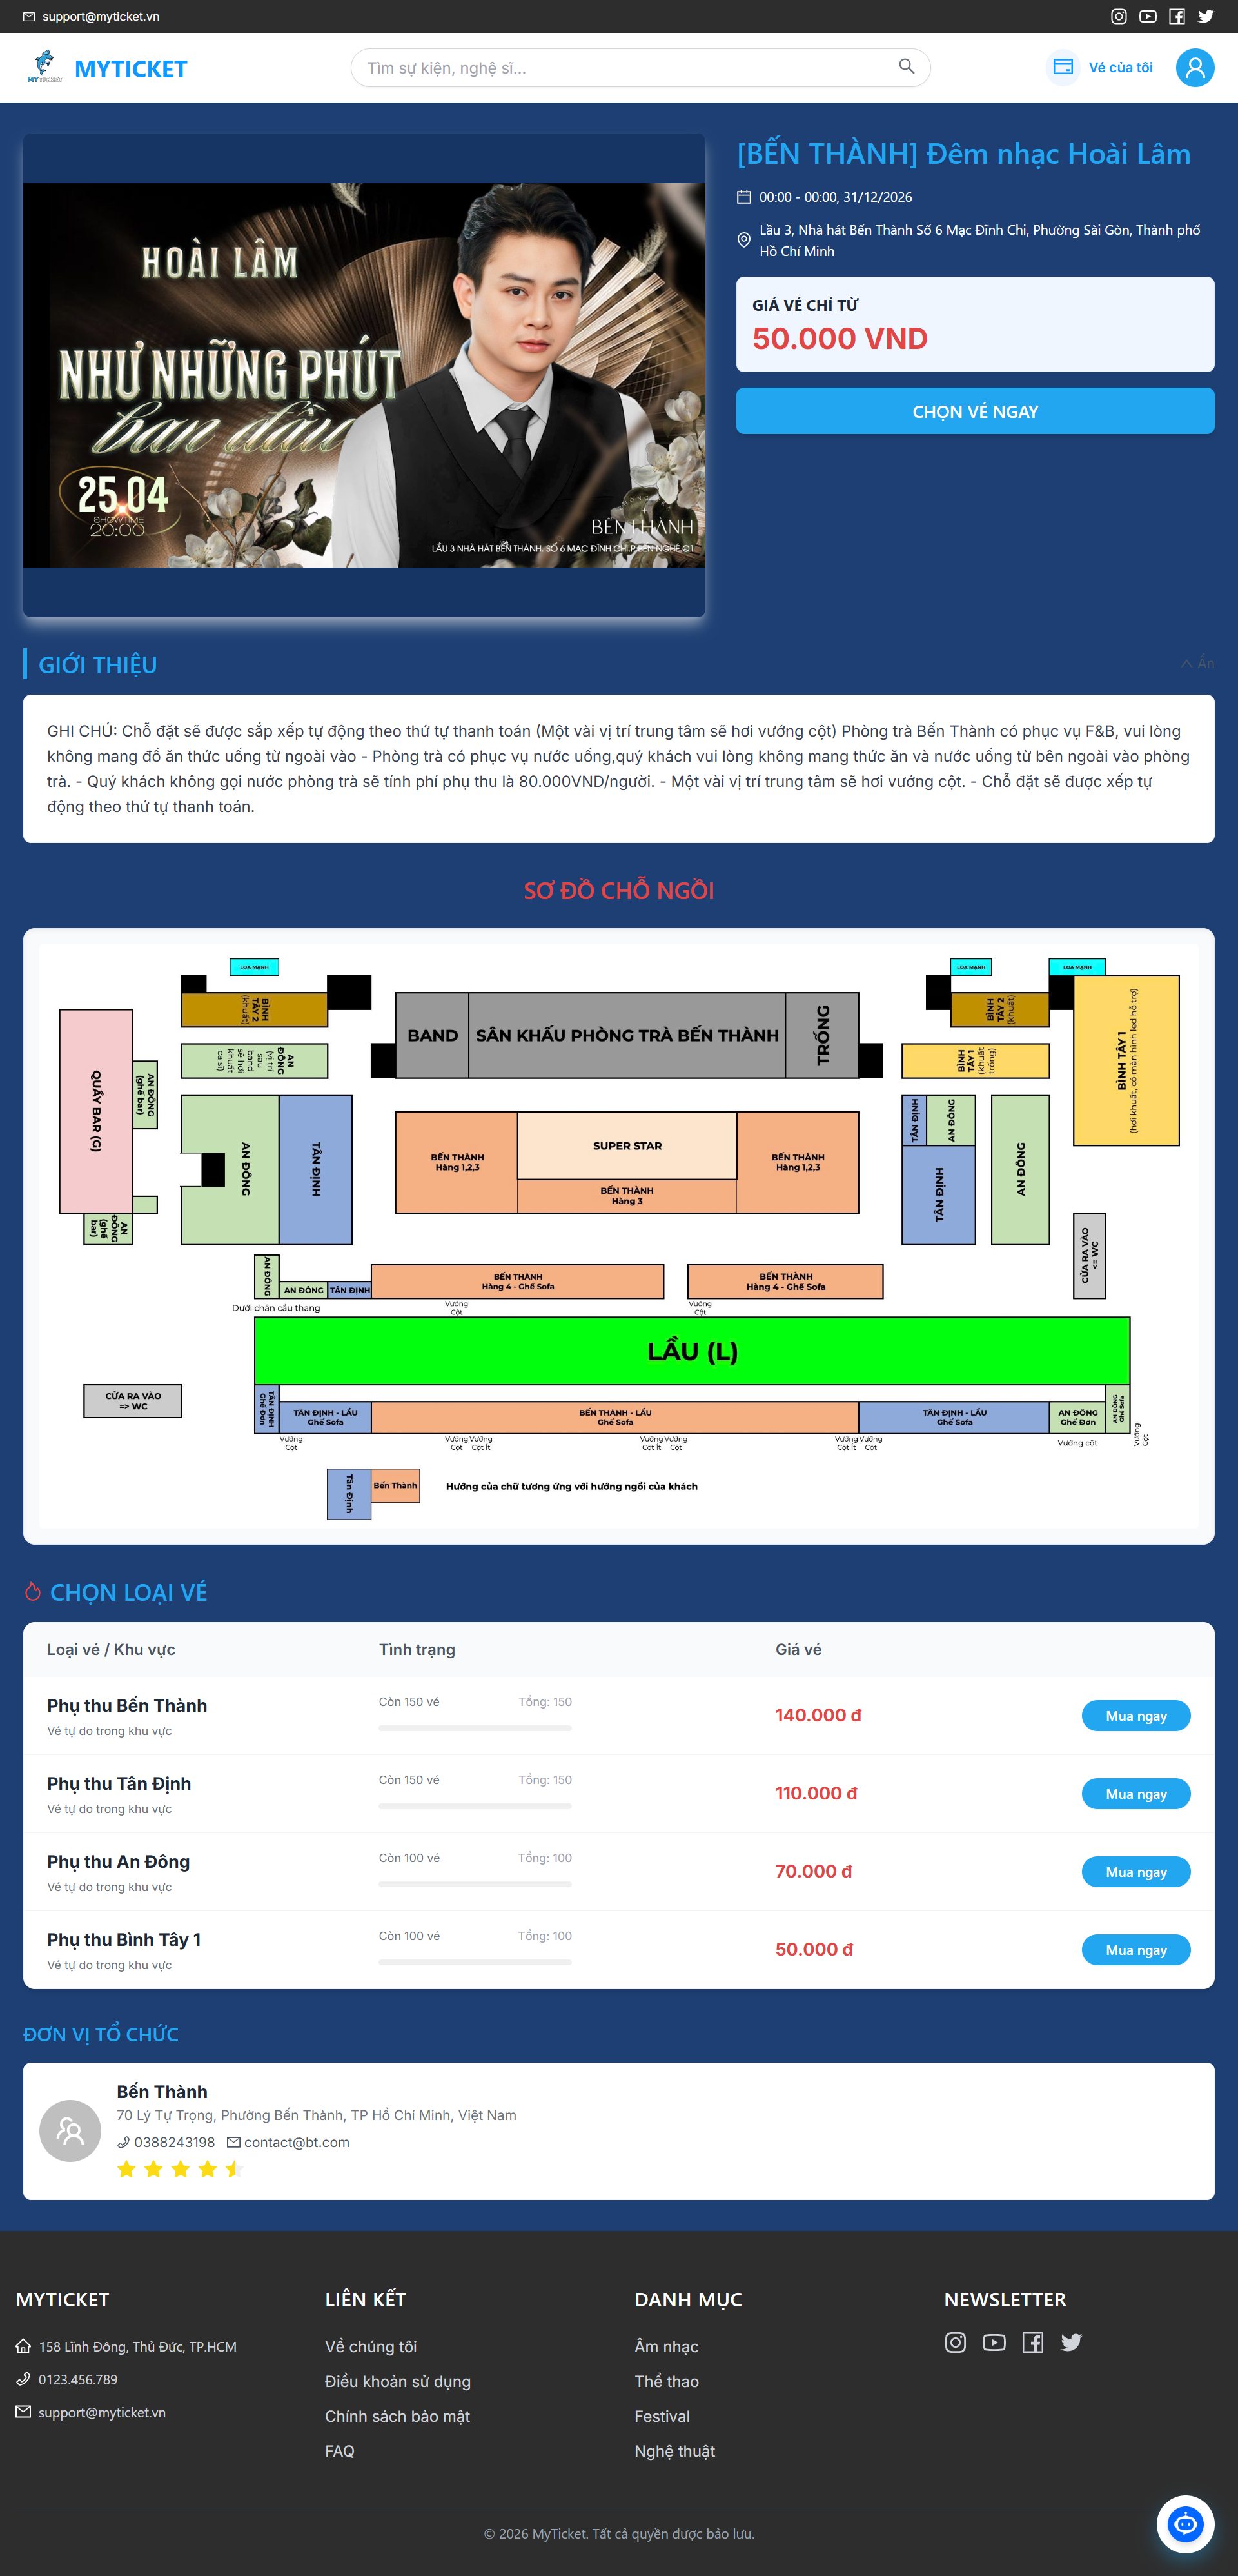
\includegraphics[width=0.650\textwidth]{Contents/UI/USER/Event Detail.png}
    \vspace{15pt}
    \caption{Giao diện hiển thị chi tiết thông tin sự kiện}
\end{figure}
\indent \indent \textbf{Mô tả:}\\
\indent - Sau khi nhấn vào nút "Xem chi tiết" của 1 sự kiện cụ thể ở trang HomePage, người dùng sẽ được điều hướng đến trang này.\\
\indent - Tại đây, người dùng có thể xem chi tiết thông tin của 1 sự kiện như địa điểm, thời gian tổ chức, mô tả, sơ đồ chỗ ngồi, bảng vé, số lượng vé kèm giá mỗi loại. \\
\indent - Nếu muốn mua vé, người dùng sẽ nhấn vào nút "Mua ngay" của một loại vé cụ thể trong bảng vé. Nếu loại vé nào đã bán hết, nút "Mua ngay" của nó sẽ bị vô hiệu hóa.
\subsubsection{Trang xác nhận thanh toán}
\begin{figure}[H]
    \centering

    \begin{subfigure}{0.51\textwidth}
        \centering
        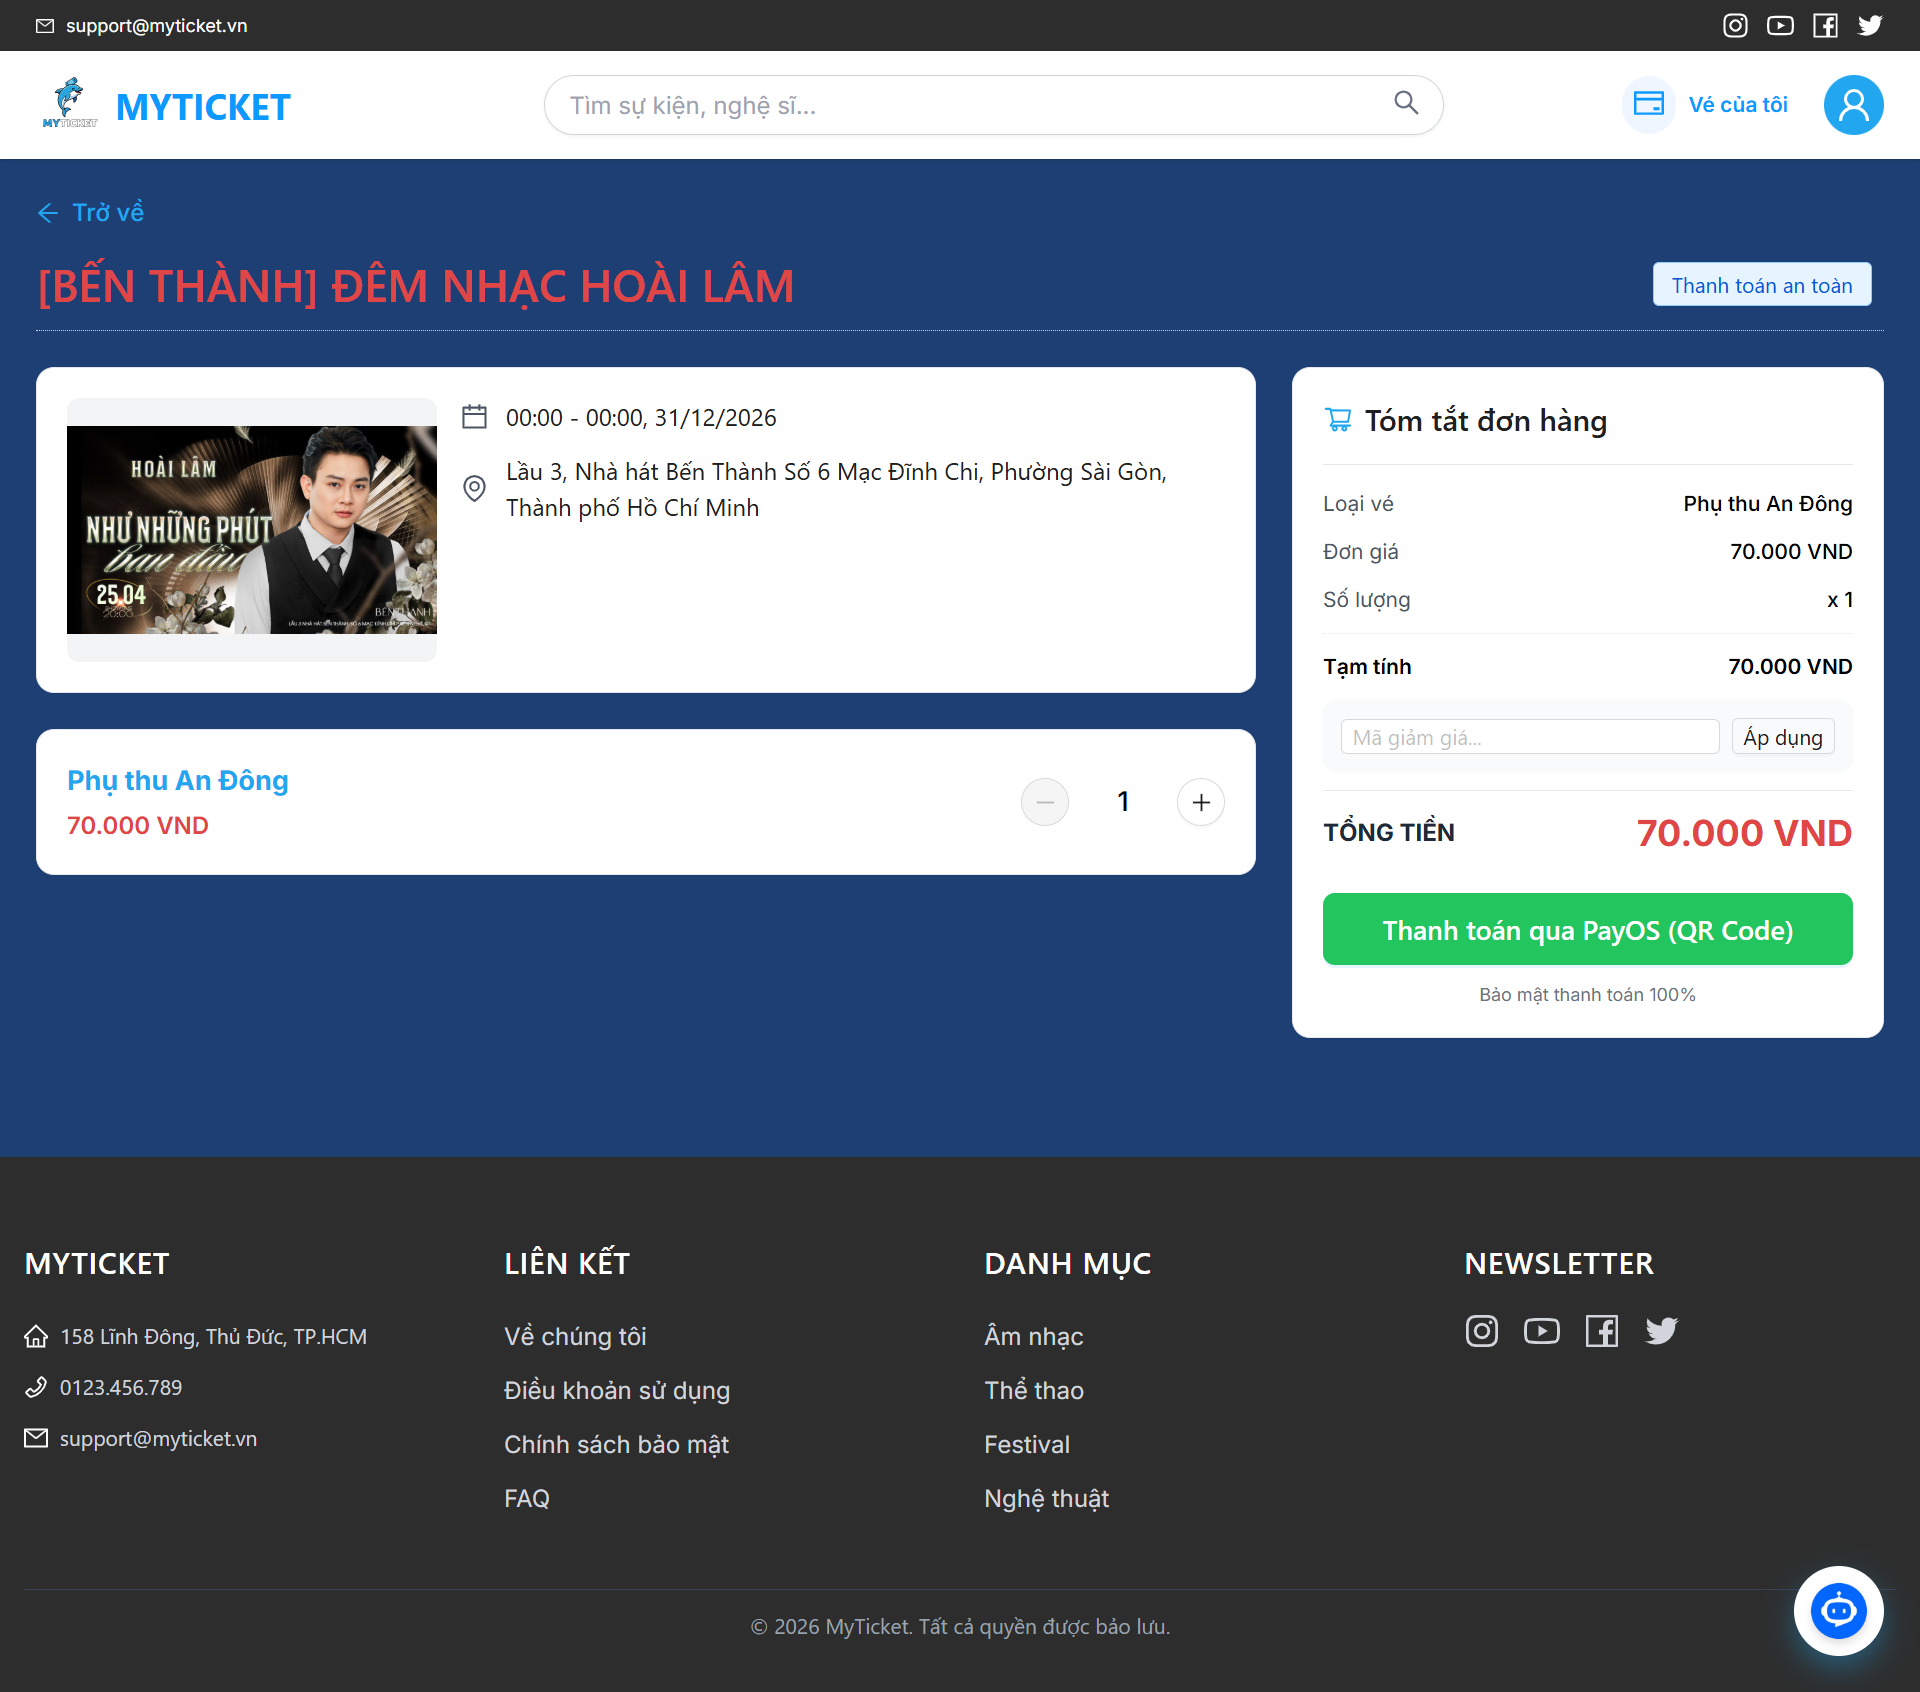
\includegraphics[width=\textwidth]{Contents/UI/USER/trang thanh toán.png}
        \caption{Trang xác nhận thanh toán với sự kiện với ghế ngồi tự do}
    \end{subfigure}
    \hfill
    \begin{subfigure}{0.44\textwidth}
        \centering
        
\includegraphics[width=\textwidth]{Contents/UI/USER/trang thanh toán_ghế cố định.png}
        \caption{Trang xác nhận thanh toán với sự kiện với ghế ngồi cố định}
    \end{subfigure}

    \vspace{15pt}
    \caption{Trang xác nhận thanh toán với các loại ghế khác nhau}
\end{figure}
\indent \indent \textbf{Mô tả:}\\
\indent - Khi chọn mua vé, người dùng sẽ được điều hướng sang trang thanh toán. \\
\indent - Tại đây, người dùng xem được các thông tin liên quan tới vé bao gồm thời gian tổ chức, địa điểm, cảnh báo độ tuổi nếu có, loại vé, số lượng, tổng giá tiền.\\
\indent - Người dùng có thể điều chỉnh số lượng vé muốn mua tùy thích miễn là có đủ số vé. \\
\indent - Đối với loại vé có chỗ ngồi cố định, người dùng được yêu cầu phải chọn thêm vị trí ghế.\\
% \indent - Đối với sự kiện có cảnh báo độ tuổi, người dùng sẽ được nhận 1 cảnh báo khi chọn nút "Xác nhận thanh toán" và phải xác nhận mới được tiến hành thanh toán.
% \begin{figure}[H]
%     \centering
%     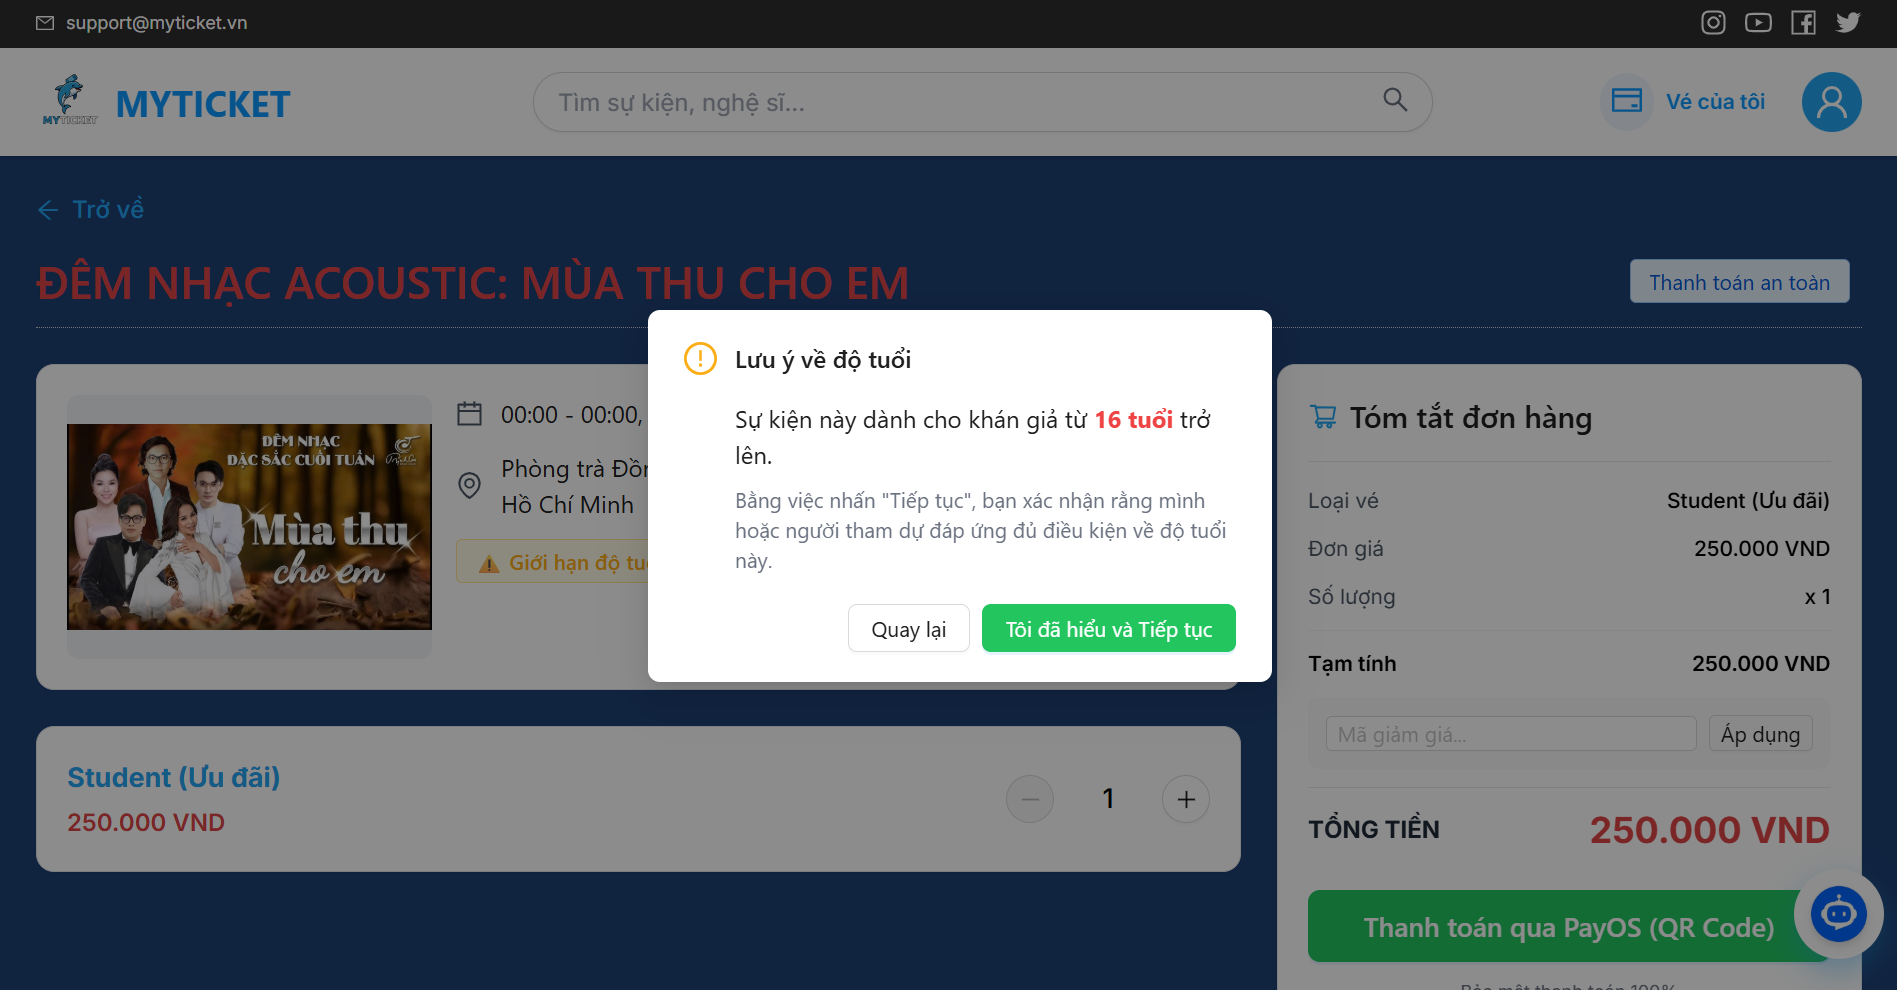
\includegraphics[width=0.65\textwidth]{Contents/UI/USER/cảnh báo độ tuổi.png}
%     \vspace{15pt}
%     \caption{Khung tin nhắn cảnh báo độ tuổi}
% \end{figure}

\subsubsection{Tiến hành thanh toán}
\begin{figure}[H]
    \centering
    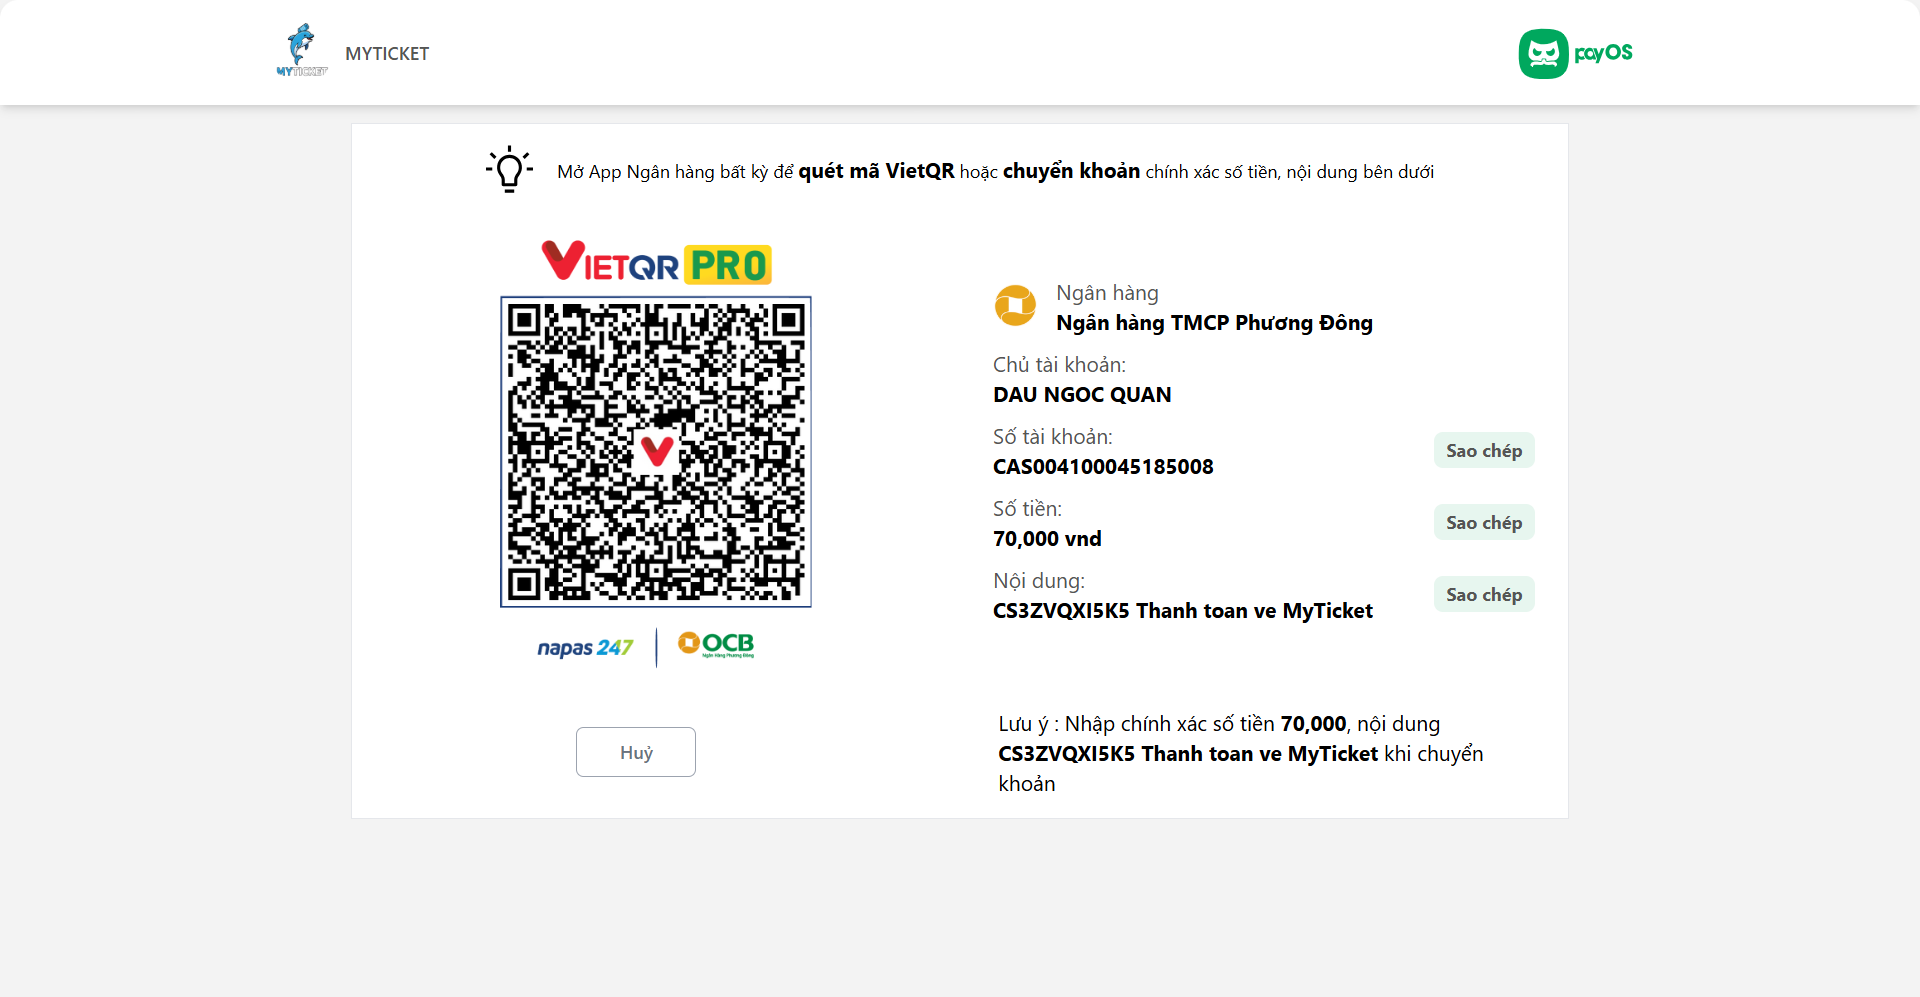
\includegraphics[width=0.65\textwidth]{Contents/UI/USER/thanh toán payos.png}
    \vspace{15pt}
    \caption{Giao diện thanh toán liên kết với PayOS}
\end{figure}
\indent \indent \textbf{Mô tả:}\\
\indent - Đây là bước cuối cùng để người dùng có thể mua vé thành công. \\
\indent - Chức năng thanh toán của hệ thống được liên kết với nền tảng PayOS. Người dùng cần dùng cái app ngân hàng hoặc ví điện tử trên điện thoại để quét mã QR và tiến hành thanh toán.\\
\indent - Sau khi thanh toán thành công, hệ thống sẽ tự động cập nhật số lượng vé đã bán và vé còn lại của sự kiện. Đồng thời, vé của người dùng sẽ được lưu vào hệ thống và người dùng sẽ được điều hướng đến trang lịch sử mua vé để xem thông tin vé vừa mua.

\subsubsection{Trang Lịch sử mua vé}
\begin{figure}[H]
    \centering
    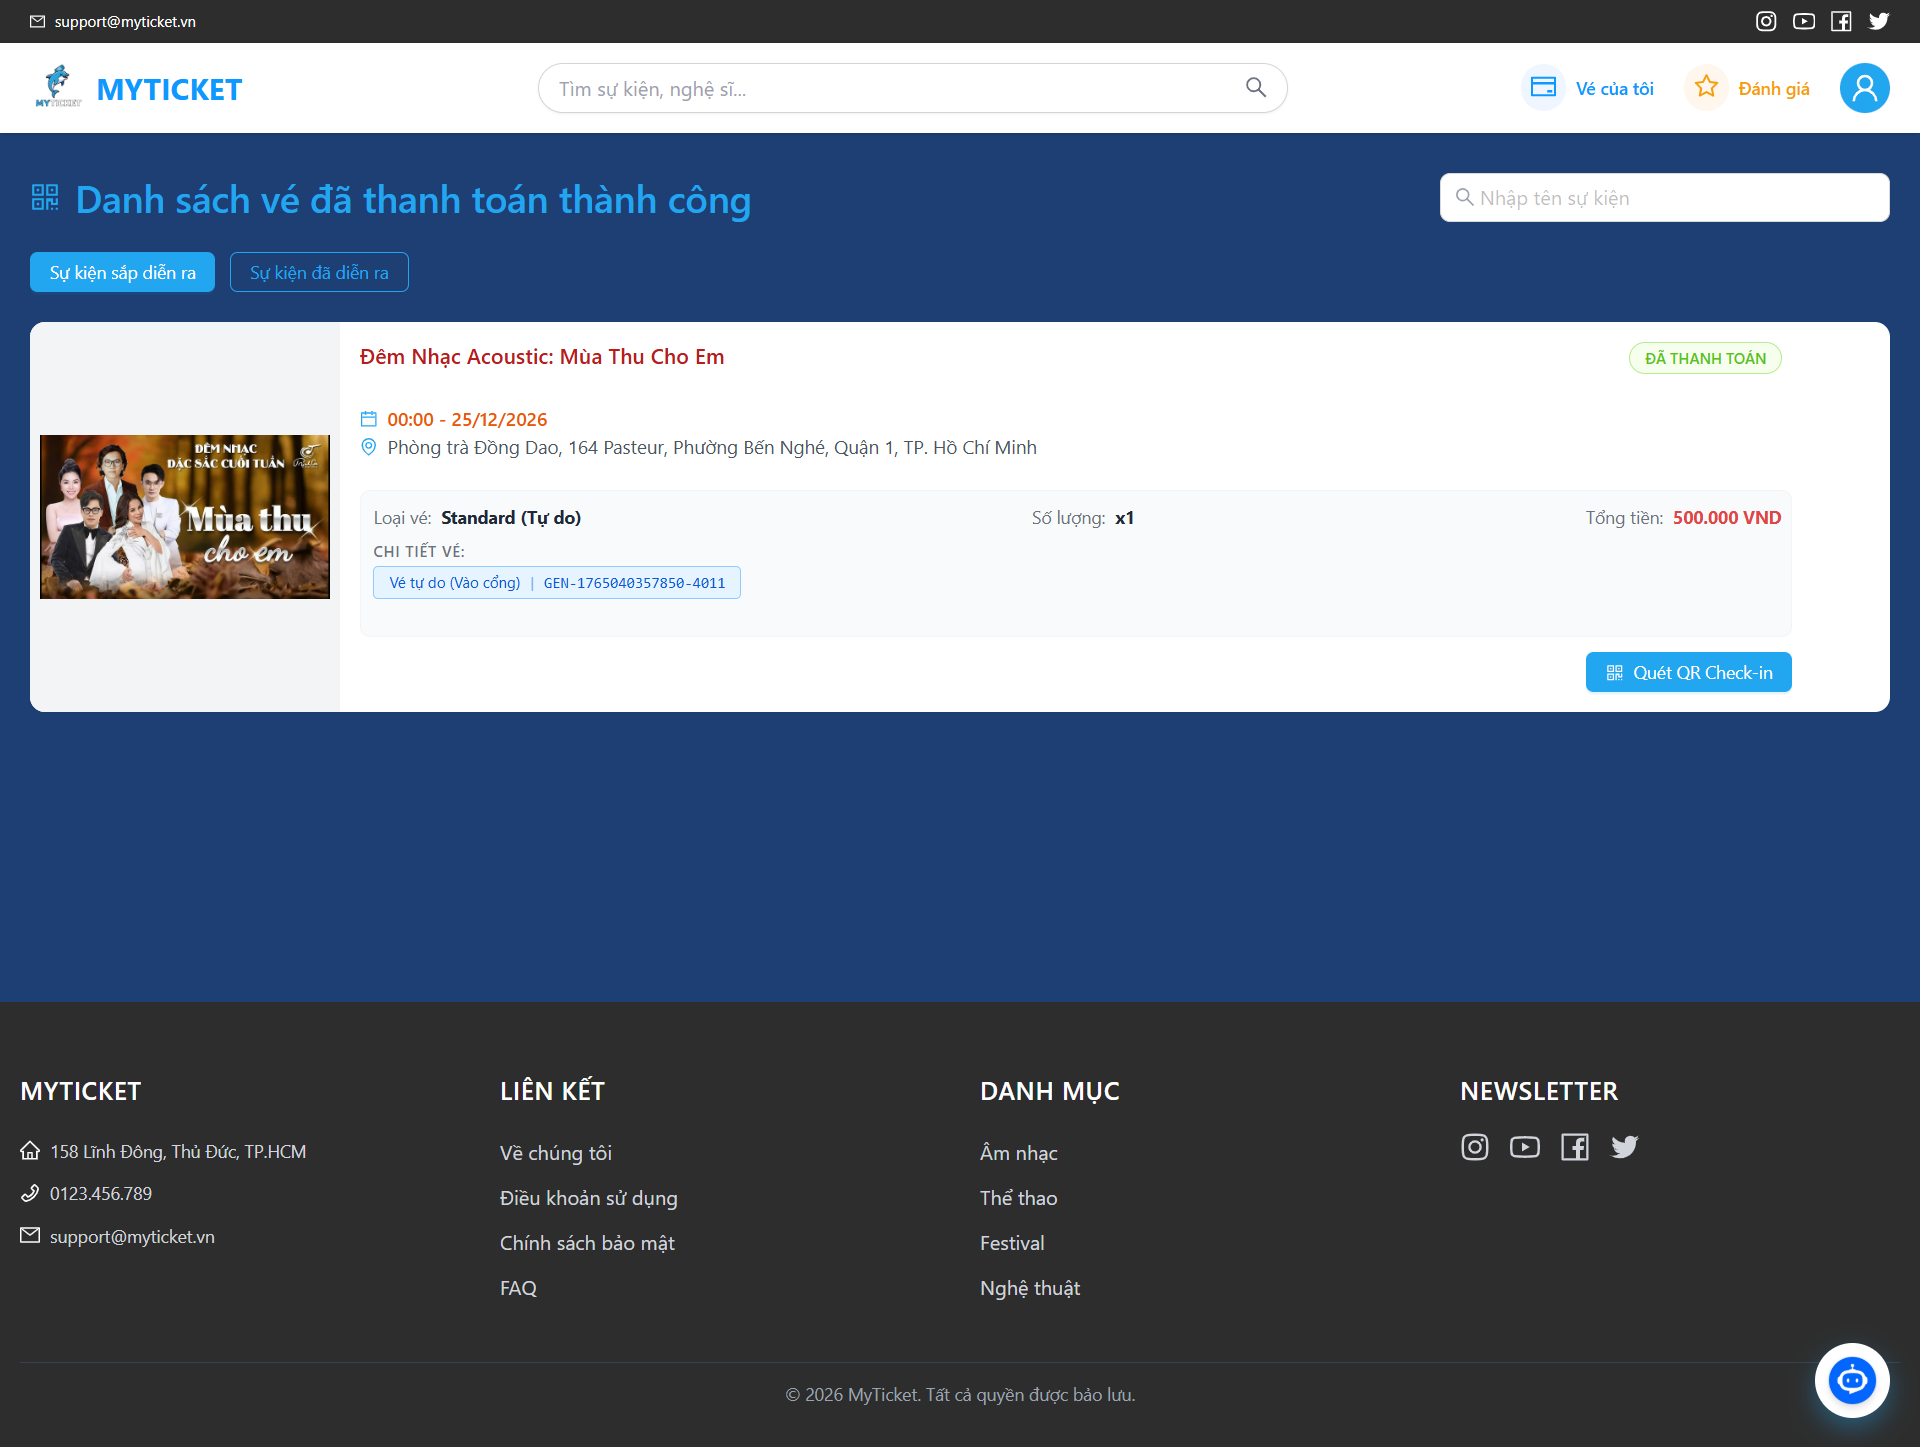
\includegraphics[width=0.65\textwidth]{Contents/UI/USER/TicketHistory1.png}
    \vspace{15pt}
    \caption{Giao diện lịch sử mua vé với sự kiện chưa diễn ra}
\end{figure}
\indent \indent \textbf{Mô tả:}\\
\indent - Sau khi người dùng mua vé thành công, vé sẽ được lưu và hệ thống tự động điều hướng người dùng đến trang này để xem thông tin vé.\\
\indent - Người dùng cũng có thể chủ động nhấn vào nút "Vé của tôi" ở header để xem lịch sử mua vé của mình miễn là đã đăng nhập thành công.\\
\indent - Tại đây, ngoài việc xem thông tin vé, người dùng còn có thể ấn vào nút "QR thông tin vé" để nhận được mã QR vé điện tử. Mã QR này sẽ được sử dụng để check-in khi người dùng đến tham dự sự kiện.

\begin{figure}[H]
    \centering
    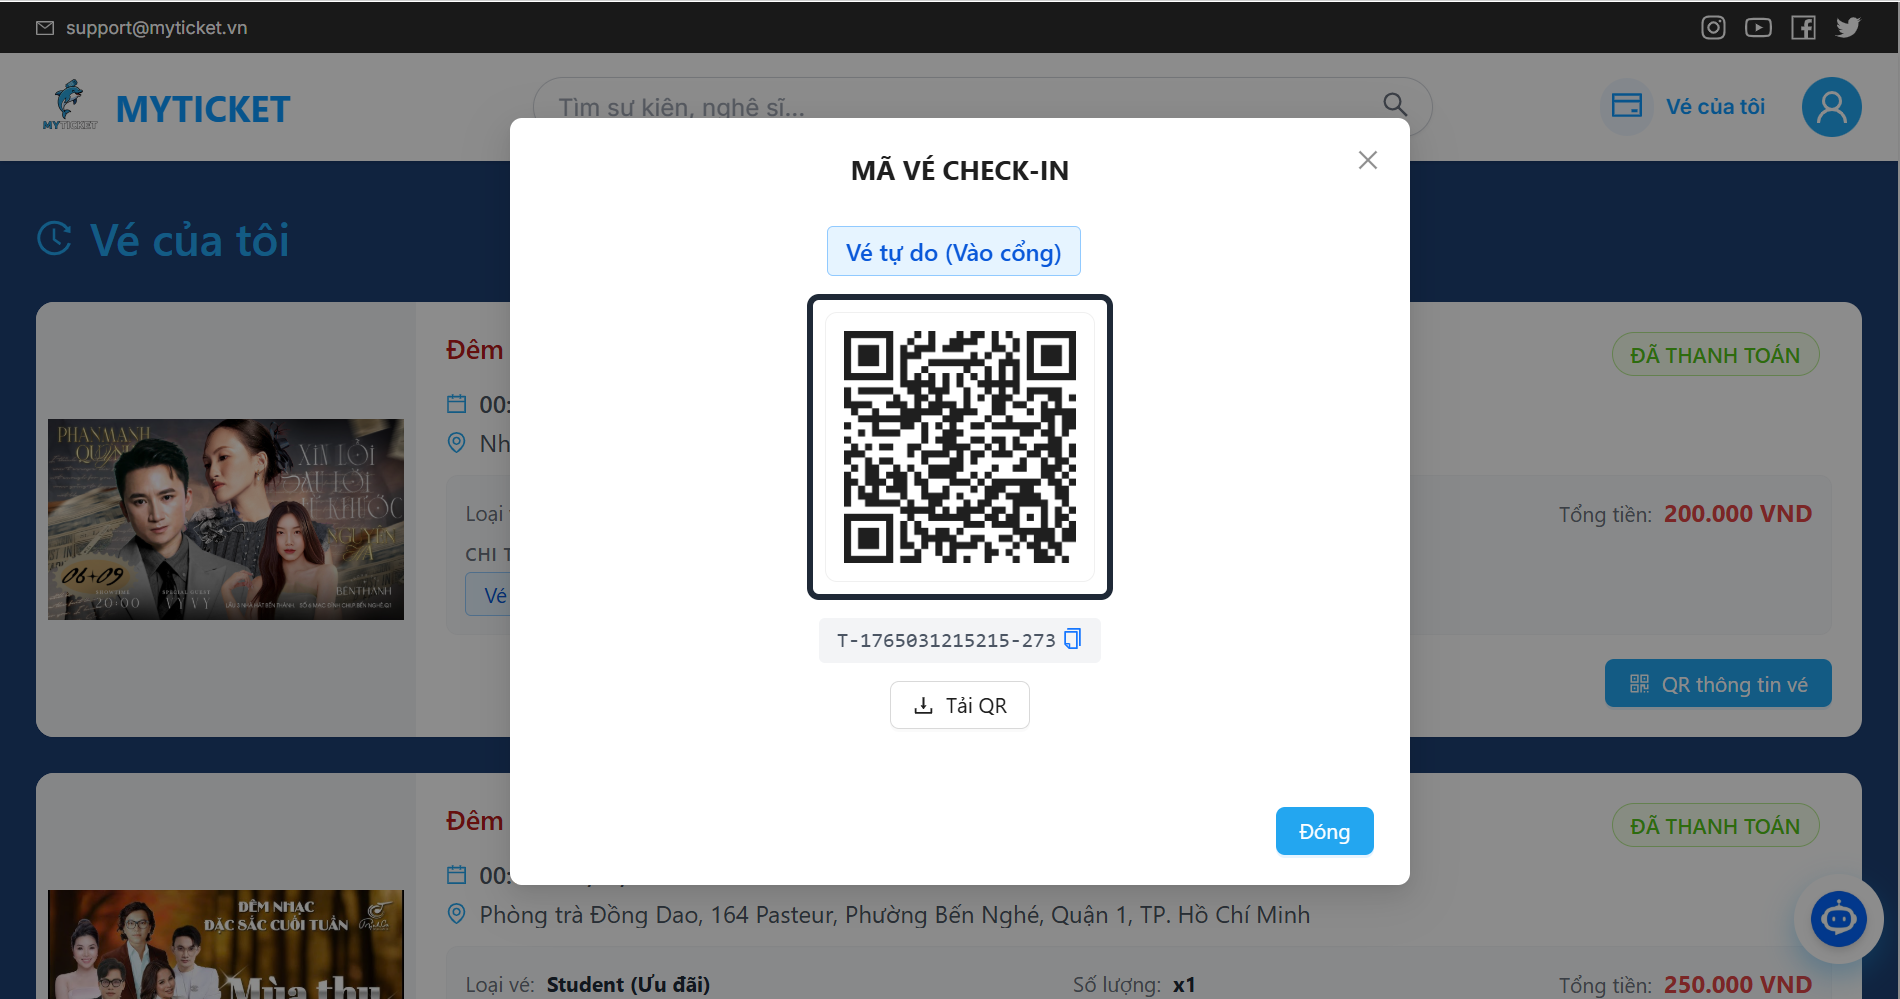
\includegraphics[width=0.65\textwidth]{Contents/UI/USER/QR e-ticket.png}
    \vspace{15pt}
    \caption{Giao diện hiển thị mã QR vé điện tử}
\end{figure}

\begin{figure}[H]
    \centering
    
\includegraphics[width=0.65\textwidth]{Contents/UI/USER/e-ticket.png}
    \vspace{15pt}
    \caption{Giao diện thông tin vé điện tử sau khi quét mã QR}
\end{figure}


\begin{figure}[H]
    \centering
    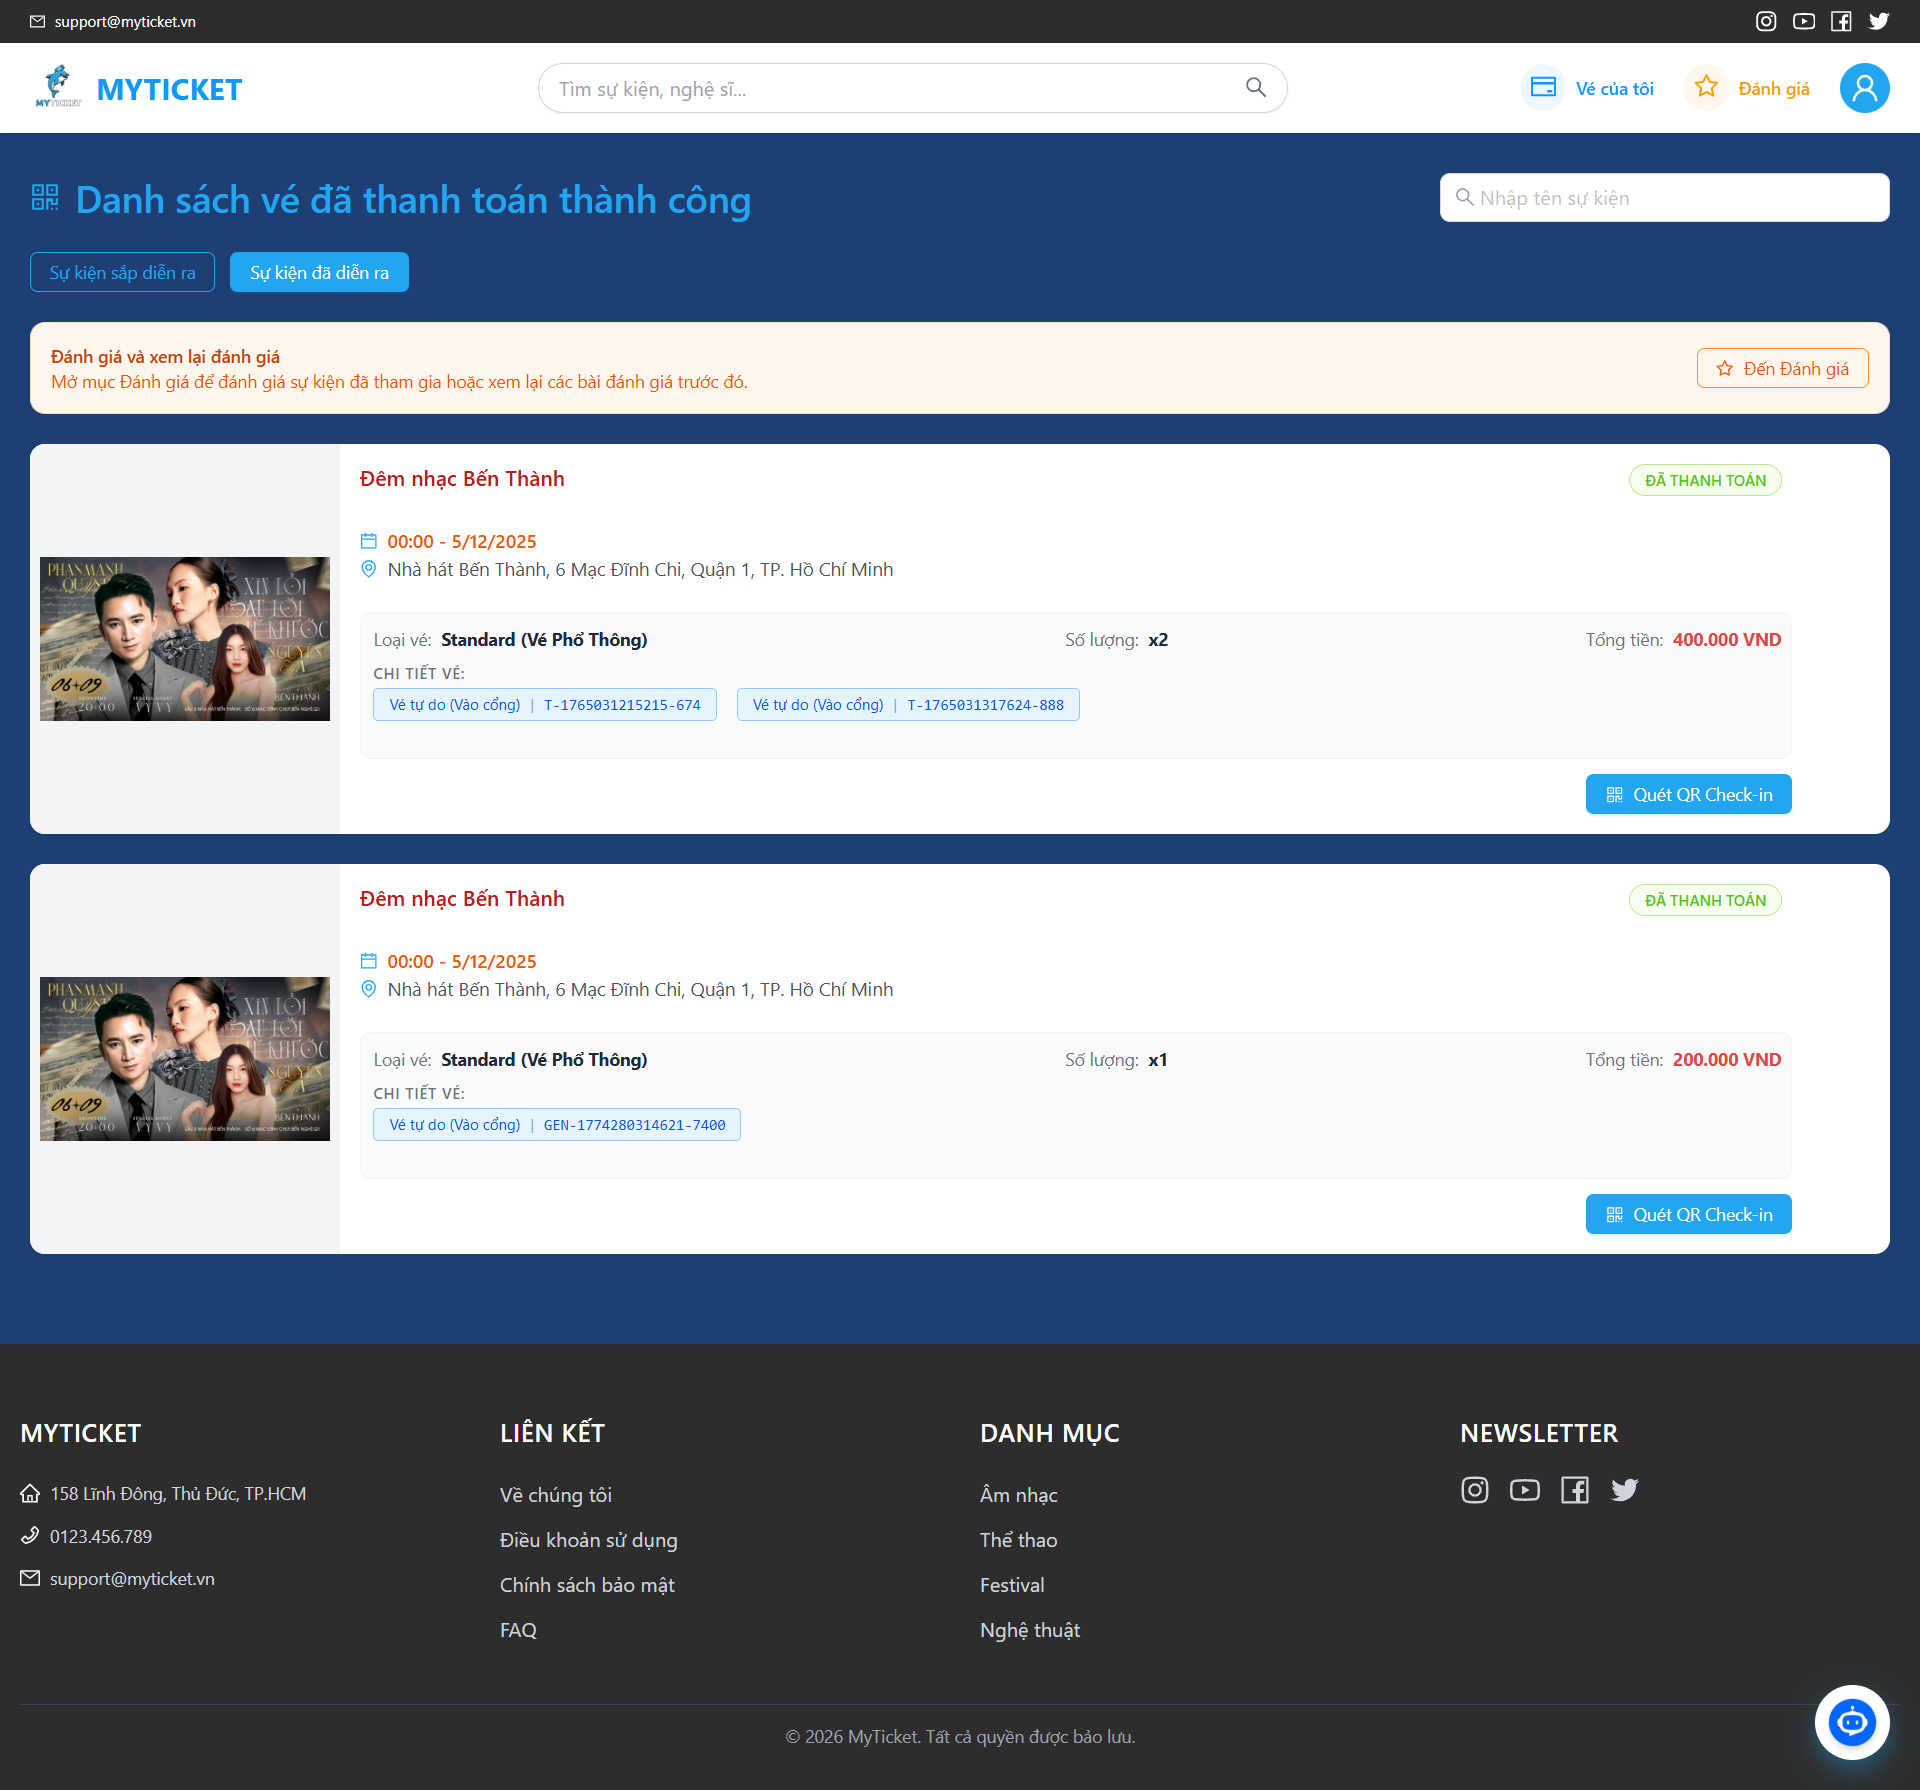
\includegraphics[width=0.65\textwidth]{Contents/UI/USER/TicketHistory2.png}
    \vspace{15pt}
    \caption{Giao diện lịch sử mua vé với sự kiện đã diễn ra để có thể đánh giá và bình luận}
\end{figure}
\indent \indent \textbf{Mô tả:}\\
\indent - Người dùng chọn nút Sự kiện đã diễn ra trên trang lịch sử mua vé.\\
\indent - Người dùng chọn nút Đến Đánh giá, hệ thống sẽ tự động điều hướng đến trang đánh giá sự kiện đã diễn ra.\\

\begin{figure}[H]
    \centering
    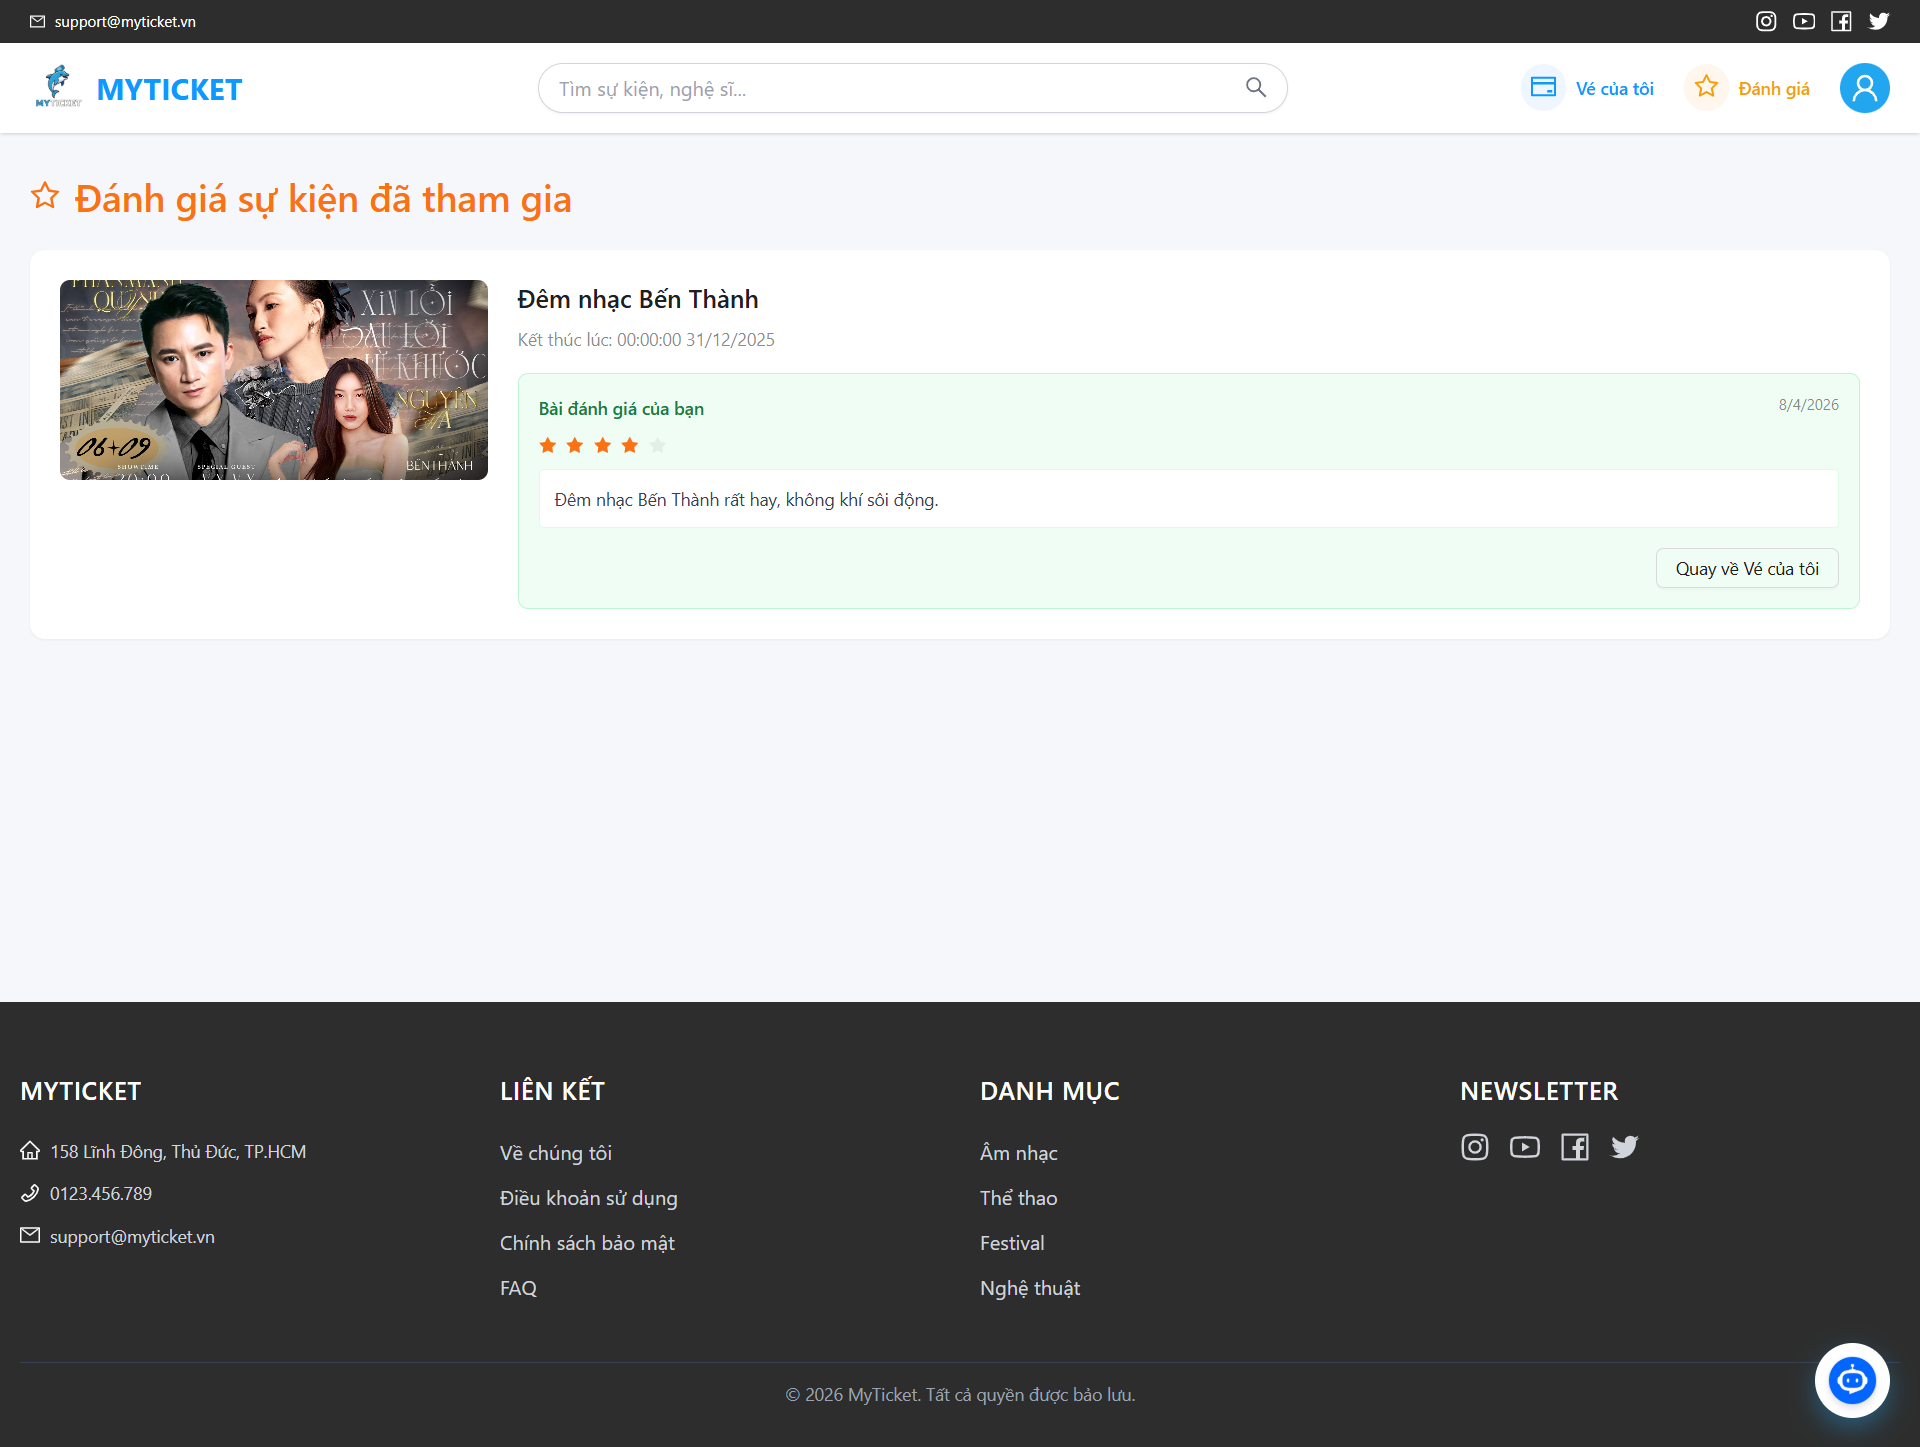
\includegraphics[width=0.65\textwidth]{Contents/UI/USER/US_Rating.png}
    \vspace{15pt}
    \caption{Giao diện trang Đánh giá sự kiện đã diễn ra}
\end{figure}
\indent \indent \textbf{Mô tả:}\\
\indent - Người dùng chọn nút Sự kiện đã diễn ra trên trang lịch sử mua vé.\\
\indent - Người dùng chọn nút Đến Đánh giá, hệ thống sẽ tự động điều hướng đến trang đánh giá sự kiện đã diễn ra.\\

\subsubsection{Trang thông tin cá nhân}
\begin{figure}[H]
    \centering
    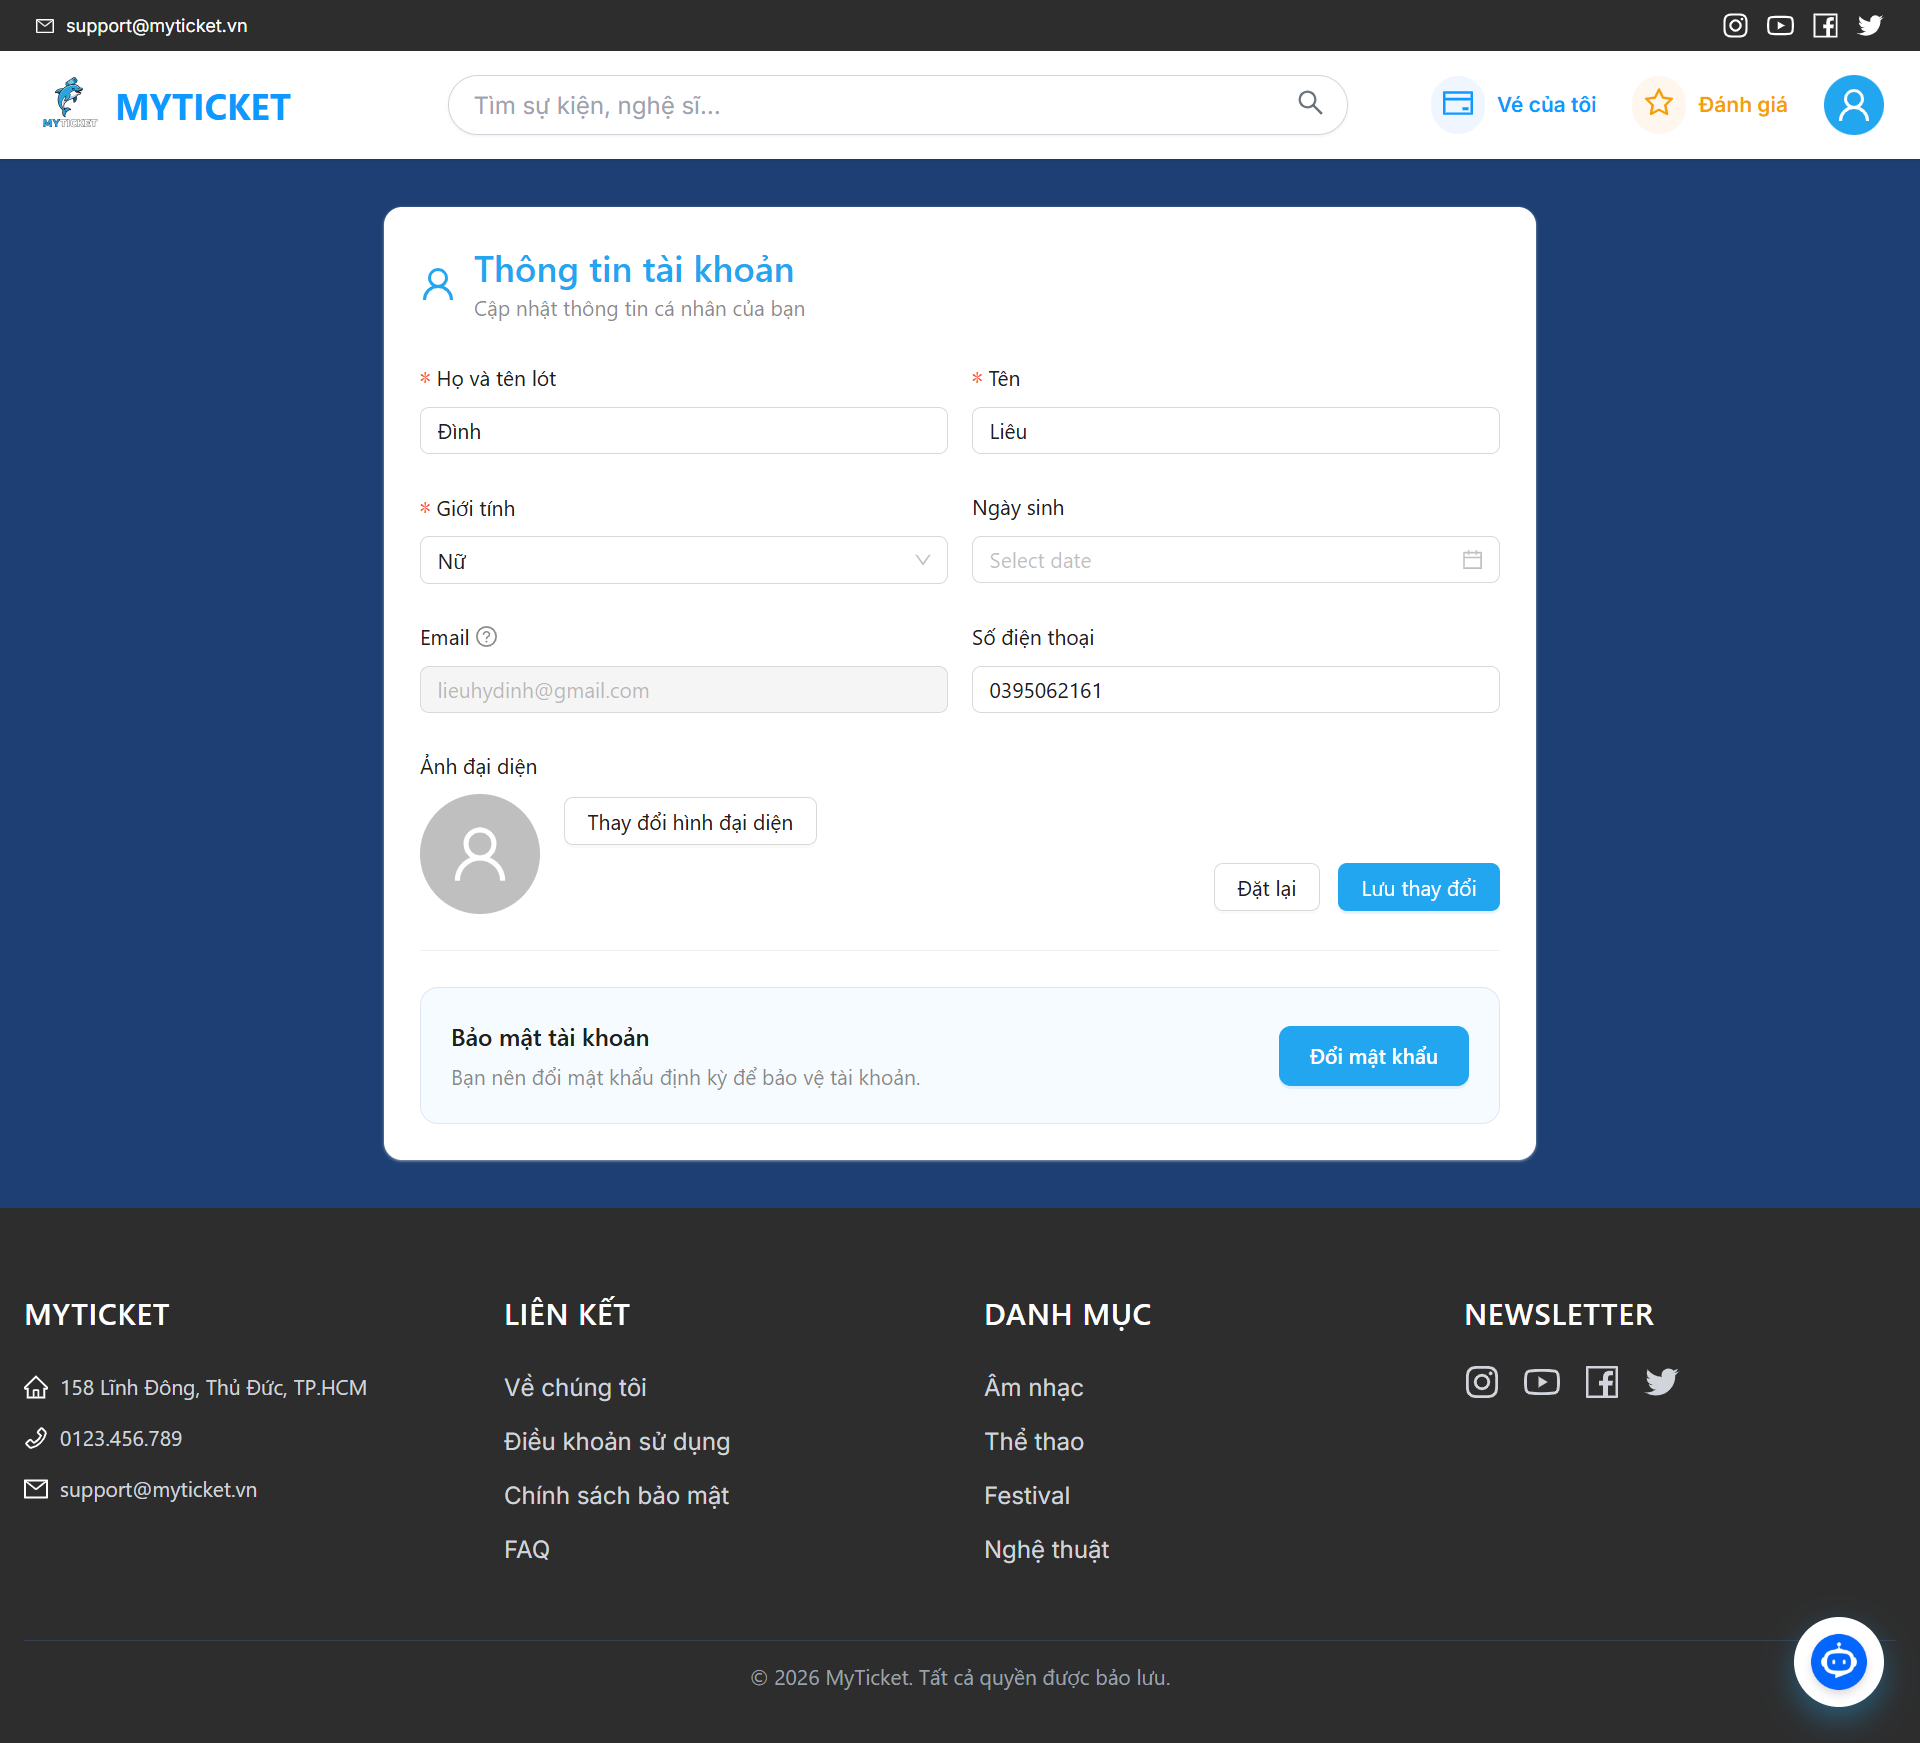
\includegraphics[width=0.6\textwidth]{Contents/UI/USER/account profile.png}
    \vspace{15pt}
    \caption{Giao diện hiển thị thông tin cá nhân của người dùng}
\end{figure}
\indent \indent \textbf{Mô tả:} \\
\indent - Người dùng cần nhấn vào avatar ở header và chọn "Thông tin tài khoản" để truy cập vào trang này.\\
\indent - Tại đây, người dùng có thể xem thông tin cá nhân của mình như tên, email, số điện thoại, v.v. \\
\indent - Để chỉnh sửa thông tin cá nhân, người dùng chỉ cần nhập thông tin mới vào các trường tương ứng hay nhấn nút "Thay đổi hình đại diện" để upload hình từ máy làm hình đại diện. Sau cùng nhấn nút "Lưu thay đổi" để lưu thay đổi. Nếu không muốn thay đổi thông tin nữa, người dùng chỉ cần nhấn nút "Đặt lại" để hoàn tác lại thông tin cũ gần nhất.\\
\indent - Ngoài ra, người dùng cũng có thể nhấn nút "Đổi mật khẩu" để chuyển sang form đổi mật khẩu nếu muốn thay đổi mật khẩu đăng nhập.

\subsection{Chức năng của Ban tổ chức sự kiện}
\indent \indent Để có thể quan sát các sự kiện được đăng tải trên hệ thống, Ban tổ chức sẽ được cấp tài khoản với role là Organizer. 
Sau khi đăng nhập thành công, hệ thống sẽ tự động điều hướng giao diện sang trang hiển thị dữ liệu thống kê tổng quan của danh sách các sự kiện do mình này tổ chức. 
\begin{figure}[H]
    \centering
    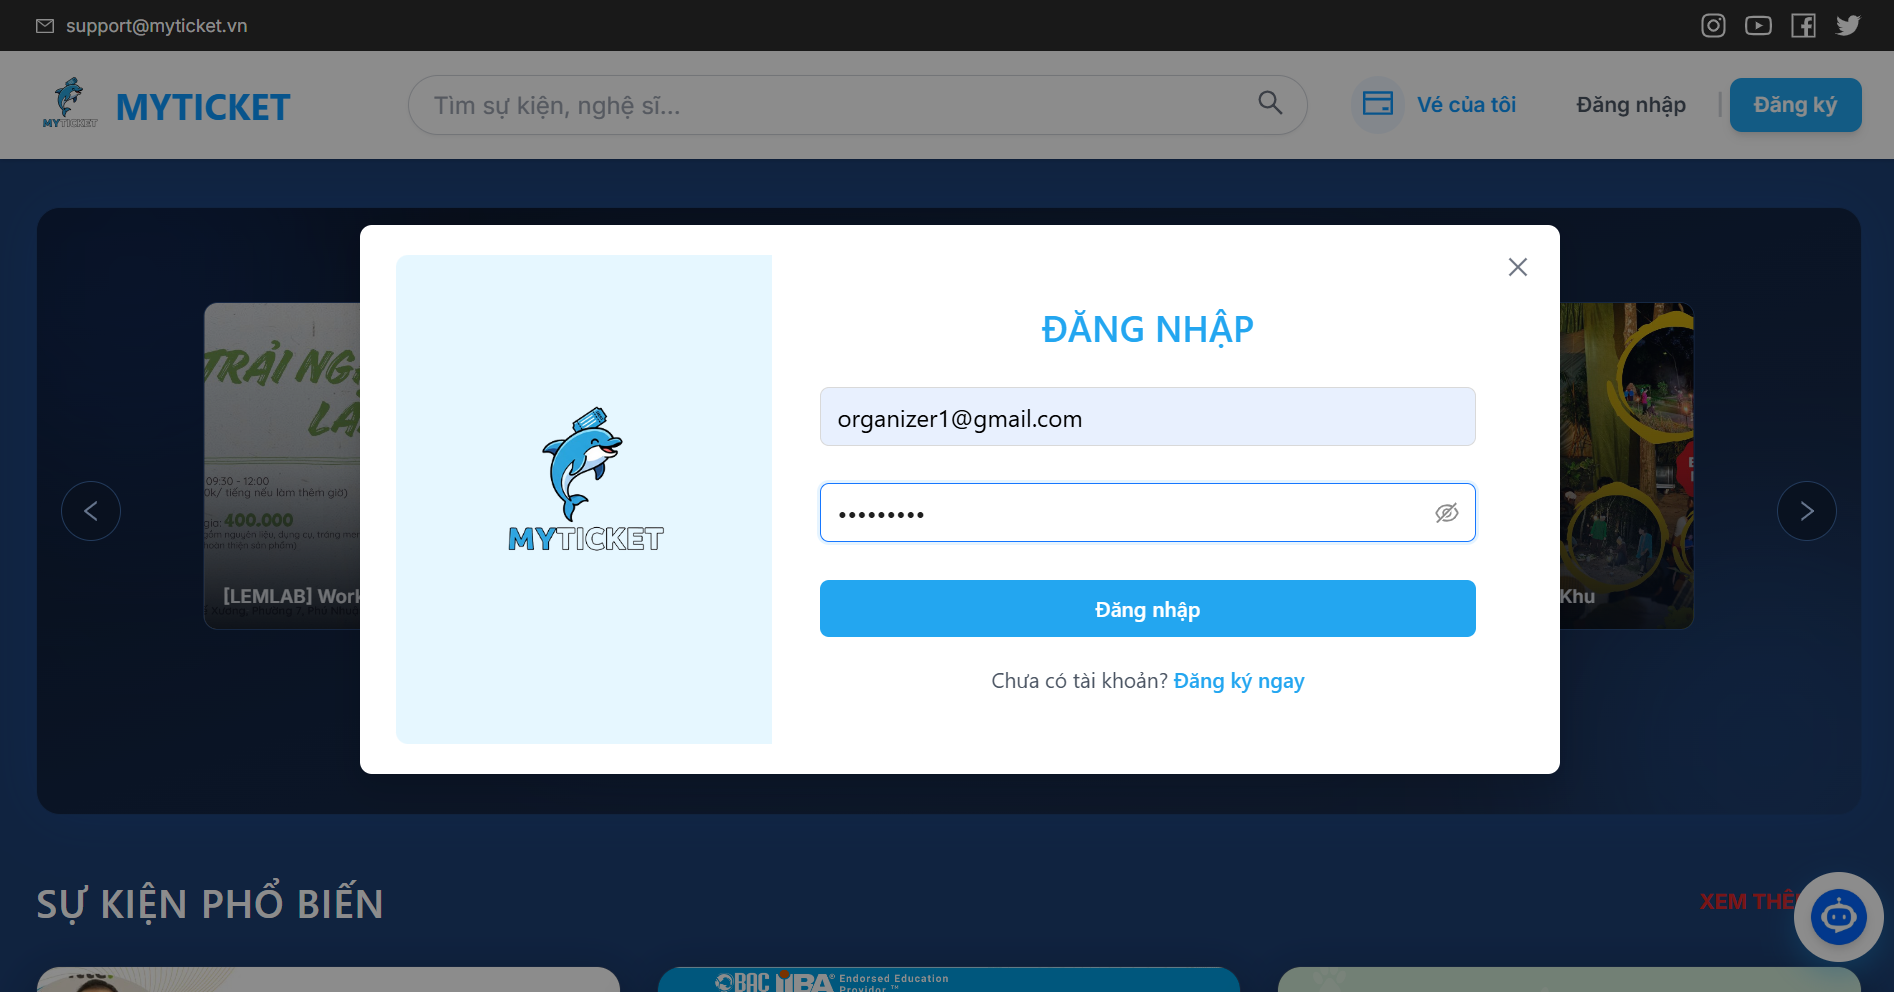
\includegraphics[width=0.65\textwidth]{Contents/UI/BTC/BTC ĐN.png}
    \vspace{15pt}
    \caption{Giao diện ban tổ chức nhập thông tin đăng nhập}
\end{figure}
% \begin{figure}[H]
%     \centering
%     
\includegraphics[width=0.65\textwidth]{Contents/UI/BTC/DL TK BTC.png}
%     \vspace{15pt}
%     \caption{Giao diện ban tổ chức sau khi đăng nhập thành công}
% \end{figure}
\indent Tại đây, Ban tổ chức có thể thực hiện các nhóm chức năng chính được mô tả chi tiết ở các phần tiếp theo.

\subsubsection{Trang dữ liệu thống kê}
\begin{figure}[H]
    \centering
    
\includegraphics[width=0.65\textwidth]{Contents/UI/BTC/DL TK BTC.png}
    \vspace{15pt}
    \caption{Giao diện hiển thị dữ liệu thống kê của Ban tổ chức}
\end{figure}
\indent \indent \textbf{Mô tả:}\\
\indent - Khi đăng nhập thành công với role Organizer, hệ thống sẽ tự động điều hướng giao diện sang trang này. Ngoài ra, Ban tổ chức cũng có thể nhấn vào mục "Statistical Data" ở thanh navbar để truy cập vào trang này.\\
\indent - Tại đây, Ban tổ chức có thể xem được các dữ liệu thống kê liên quan đến các sự kiện do mình tổ chức như số lượng vé đã bán, số lượng vé còn lại, doanh thu, v.v.
\subsubsection{Trang thông tin sự kiện}
\begin{figure}[H]
    \centering
    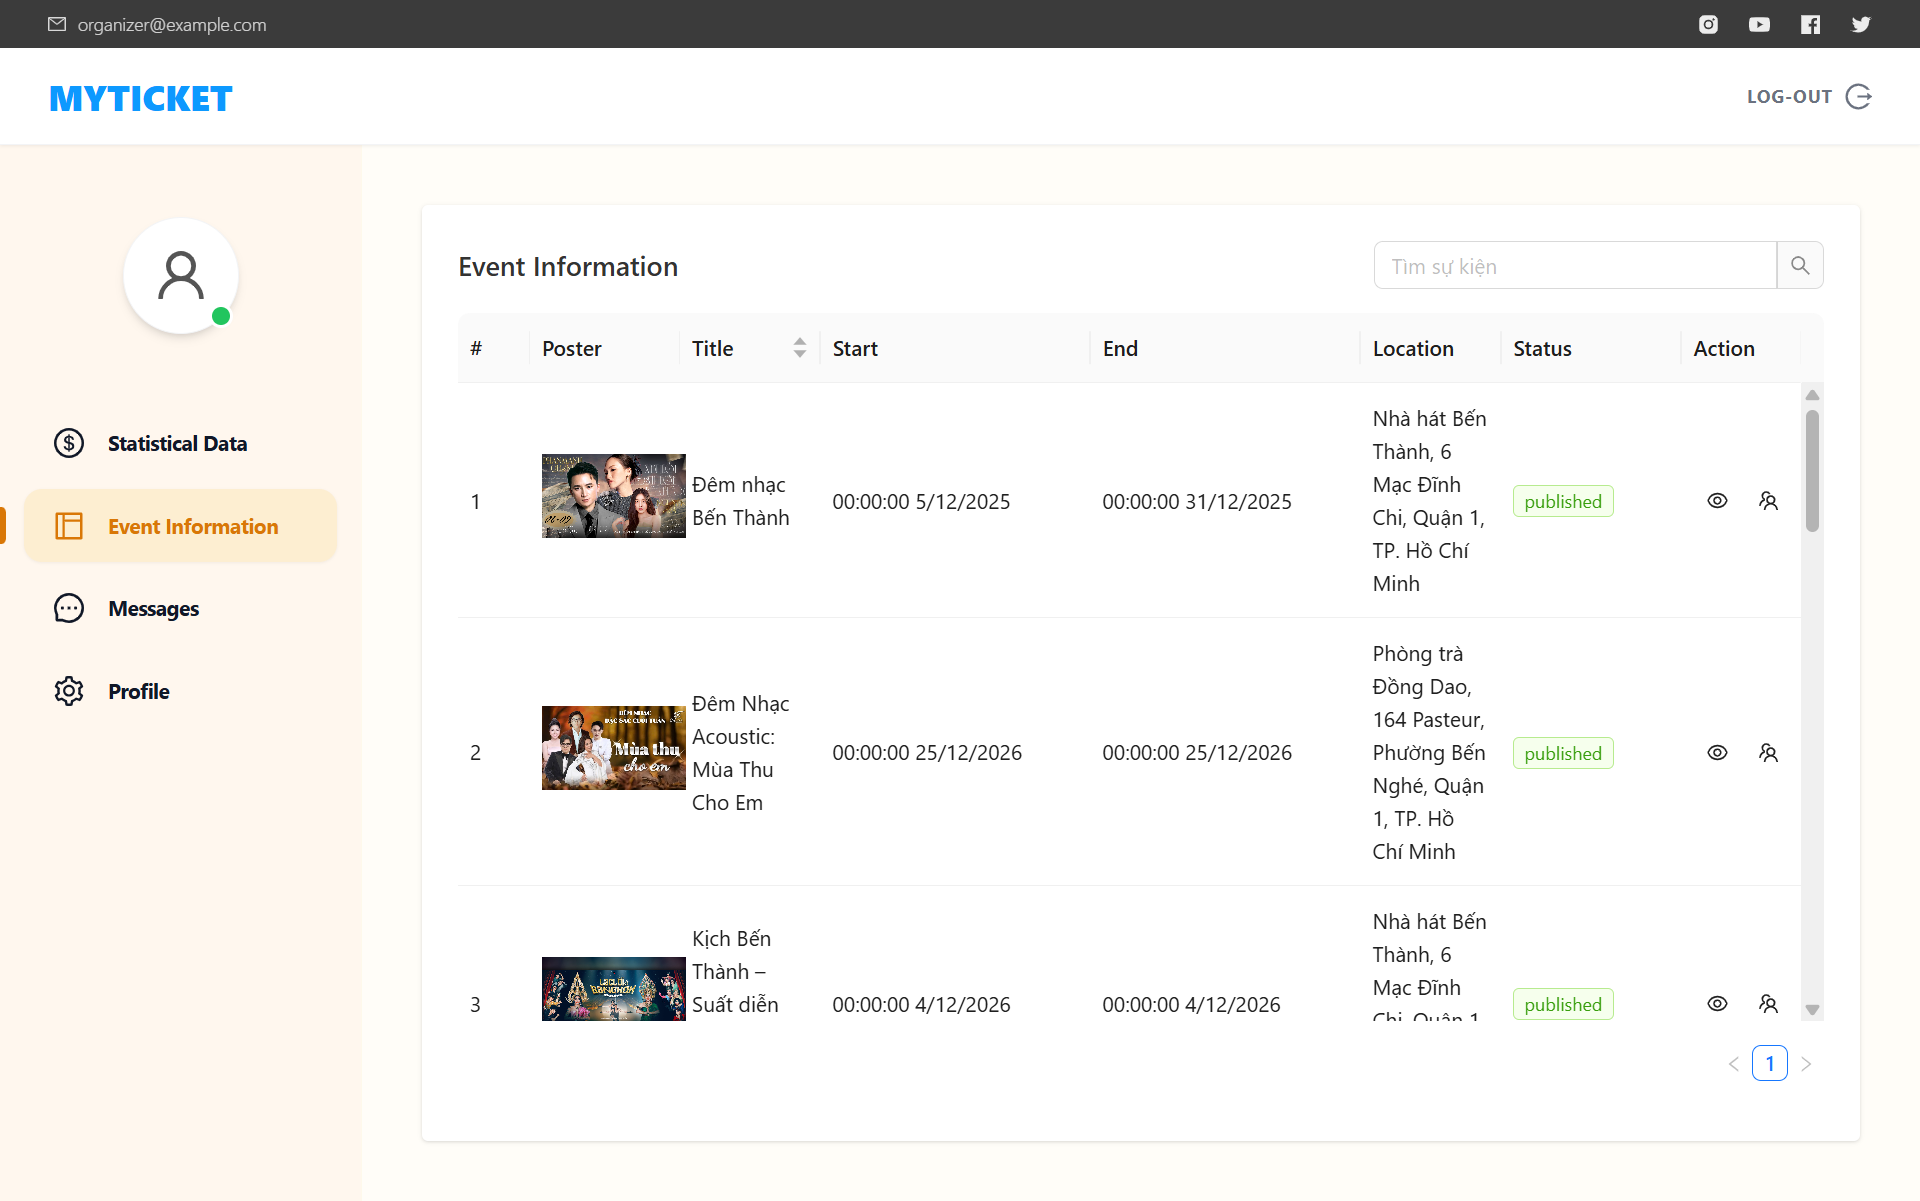
\includegraphics[width=0.65\textwidth]{Contents/UI/BTC/Giao diện BTC.png}
    \vspace{15pt}
    \caption{Giao diện hiển thị danh sách các sự kiện tổng quan của Ban tổ chức}
\end{figure}

\begin{figure}[H]
    \centering
    
\includegraphics[width=0.65\textwidth]{Contents/UI/BTC/Xem TT SK.png}
    \vspace{15pt}
    \caption{Giao diện hiển thị chi tiết thông tin một sự kiện cụ thể của Ban tổ chức}
\end{figure}
\indent \indent \textbf{Mô tả:}\\
\indent - Ban tổ chức cần nhấn vào mục "Event Information" ở thanh navbar để truy cập vào trang này.\\
\indent - Tại đây, Ban tổ chức có thể xem danh sách các sự kiện tổng quan do mình tổ chức được đăng tải trên hệ thống bằng cách cuộn hoặc click vào icon eye của cột action của một sự kiện cụ thể để xem bảng thông tin chi tiết.\\
\indent - Để tiện lợi cho việc xem thông tin sự kiện, Ban tổ chức có thể tìm kiếm bằng tên sự kiện trên thanh tìm kiếm.

\begin{figure}[H]
    \centering
    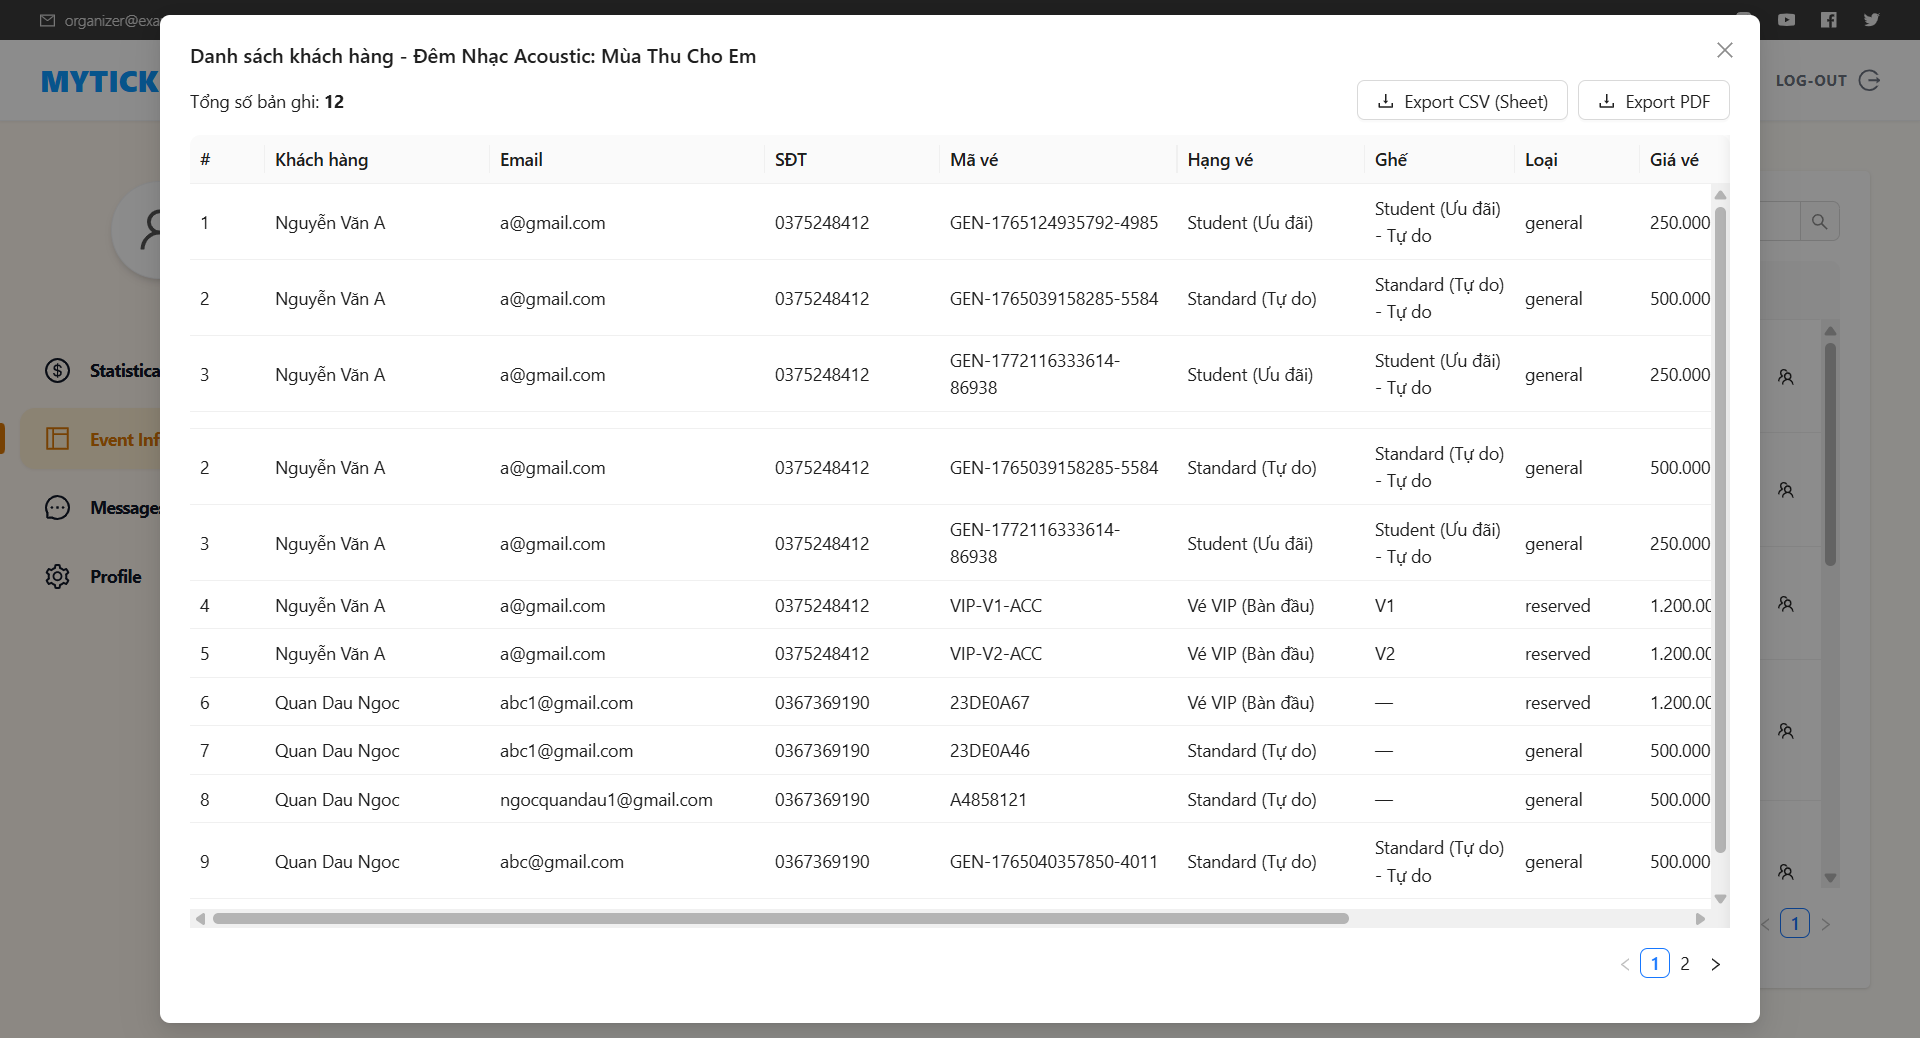
\includegraphics[width=0.65\textwidth]{Contents/UI/BTC/List_us.png}
    \vspace{15pt}
    \caption{Giao diện hiển thị danh sách khách hàng}
\end{figure}
\indent \indent \textbf{Mô tả:}\\
\indent - Ban tổ chức cần nhấn vào biểu tượng người dùng ở thanh cột Action để truy cập vào trang này.\\

\begin{figure}[H]
    \centering
    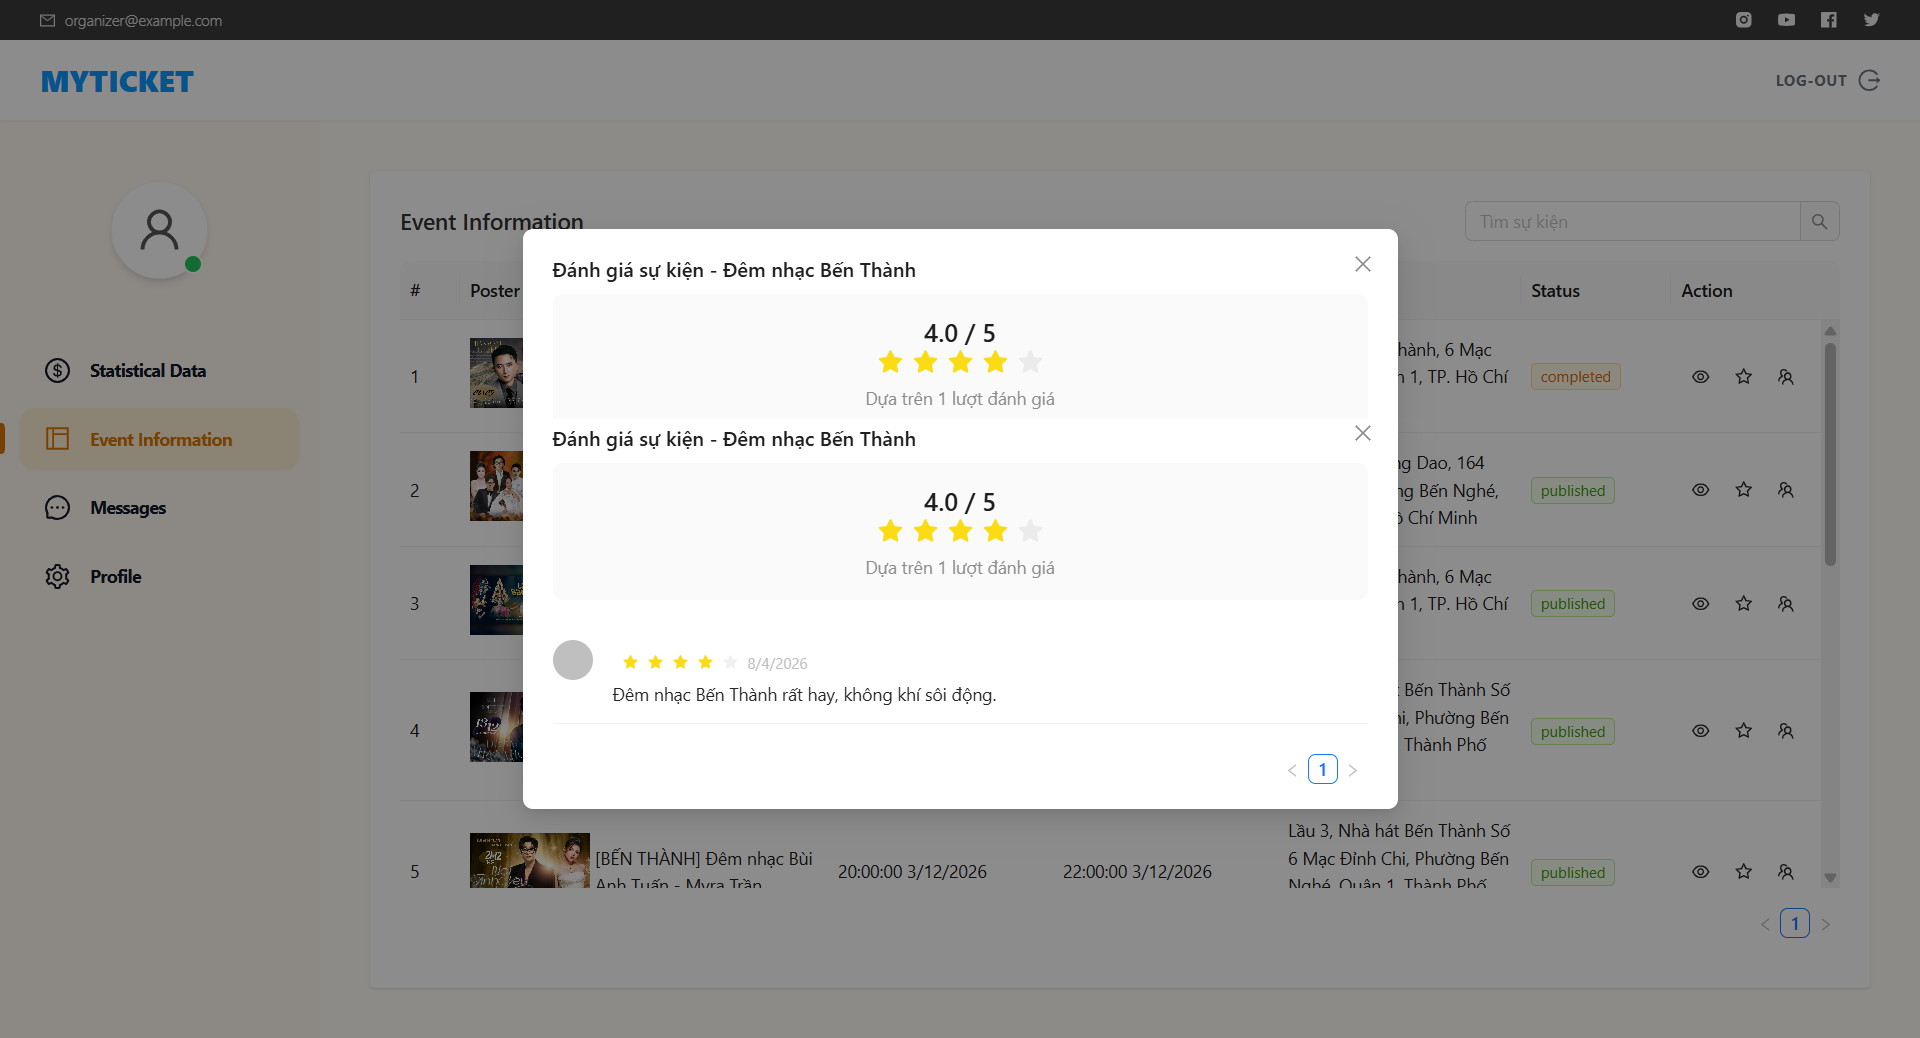
\includegraphics[width=0.65\textwidth]{Contents/UI/BTC/Org_Rating.png}
    \vspace{15pt}
    \caption{Giao diện hiển thị danh sách đánh giá}
\end{figure}
\indent \indent \textbf{Mô tả:}\\
\indent - Ban tổ chức cần nhấn vào biểu tượng ngôi sao ở thanh cột Action để truy cập vào trang này.\\


\subsubsection{Trang thông tin cá nhân}
\begin{figure}[H]
    \centering
    
\includegraphics[width=0.65\textwidth]{Contents/UI/BTC/Thông tin BTC.png}
    \vspace{15pt}
    \caption{Giao diện hiển thị thông tin cá nhân của Ban tổ chức}
\end{figure}
\indent \indent \textbf{Mô tả:} \\
\indent - Ban tổ chức cần nhấn vào mục "Profile" ở thanh navbar để truy cập vào trang này.\\
\indent - Tại đây, Ban tổ chức có thể xem thông tin cá nhân của mình như tên, email, số điện thoại, v.v. Ban tổ chức có thể nhấn nút "Refresh" để cập nhật lại thông tin cá nhân nếu có sự thay đổi.

% \subsubsection{Chat giữa Ban tổ chức và người dùng}
% \begin{figure}[H]
%     \centering
%     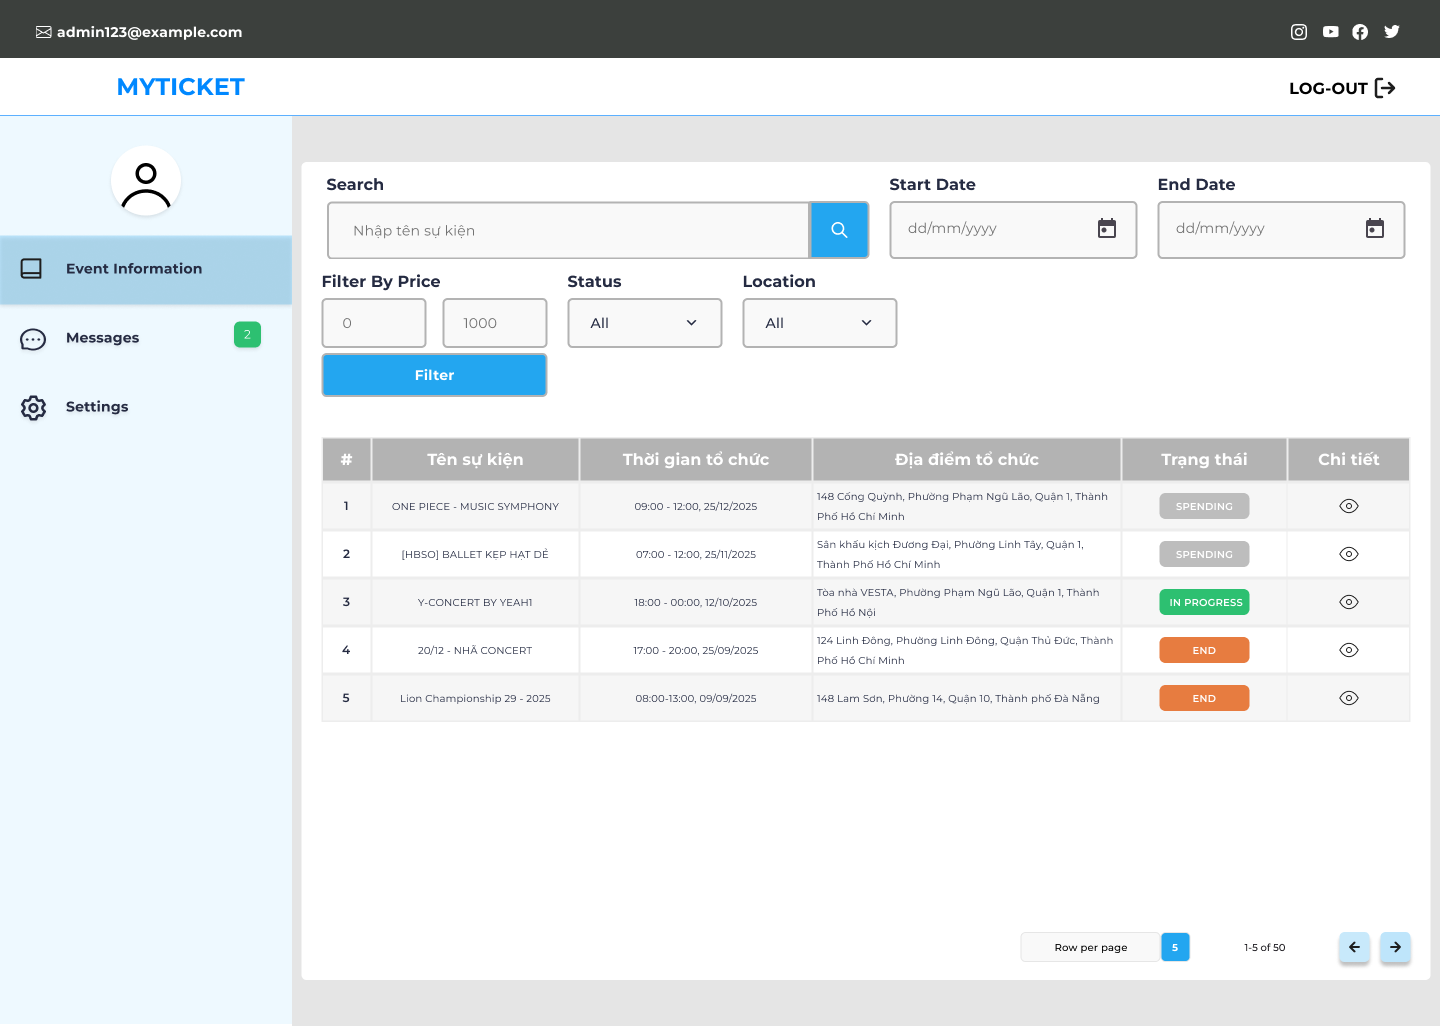
\includegraphics[width=0.65\textwidth]{Contents/UI/BTC/Ban tổ chức - Danh sách sự kiện (1).png}
%     \vspace{15pt}
%     \caption{Giao diện khung chat giữa Ban tổ chức và người dùng}
% \end{figure}
% \indent \indent Mô tả:
% \indent - Số lượng tin nhắn chưa được đọc sẽ luôn được cập nhật tự động ở mục "Messages".\\
% \indent - Tạo mục "Messages", Ban tổ chức sẽ được danh sách các người dùng có tin nhắn.\\
% \indent - Các tin nhắn mới chưa đọc sẽ được hiển thị kèm dấu chấm xanh để tiện theo dõi. Khi được đọc, dấu chấm xanh sẽ tự động biến mất.\\
% \indent - Sau khi Ban tổ chức chọn 1 người dùng cụ thể, hệ thống sẽ hiển thị giao diện khung chat cho phép phản hồi.
\subsection{Chức năng của Quản trị viên}

\indent \indent Để có thể quan sát và thực hiện nhóm chức năng quản lý cho sự kiện, vé, ban tổ chức hay người dùng trên hệ thống, Quản trị viên sẽ được cấp tài khoản với role là Admin. 
Sau khi đăng nhập thành công, hệ thống sẽ tự động điều hướng giao diện sang trang hiển thị dữ liệu thống kê tổng quan của danh sách các sự kiện trên hệ thống. 
\begin{figure}[H]
    \centering
    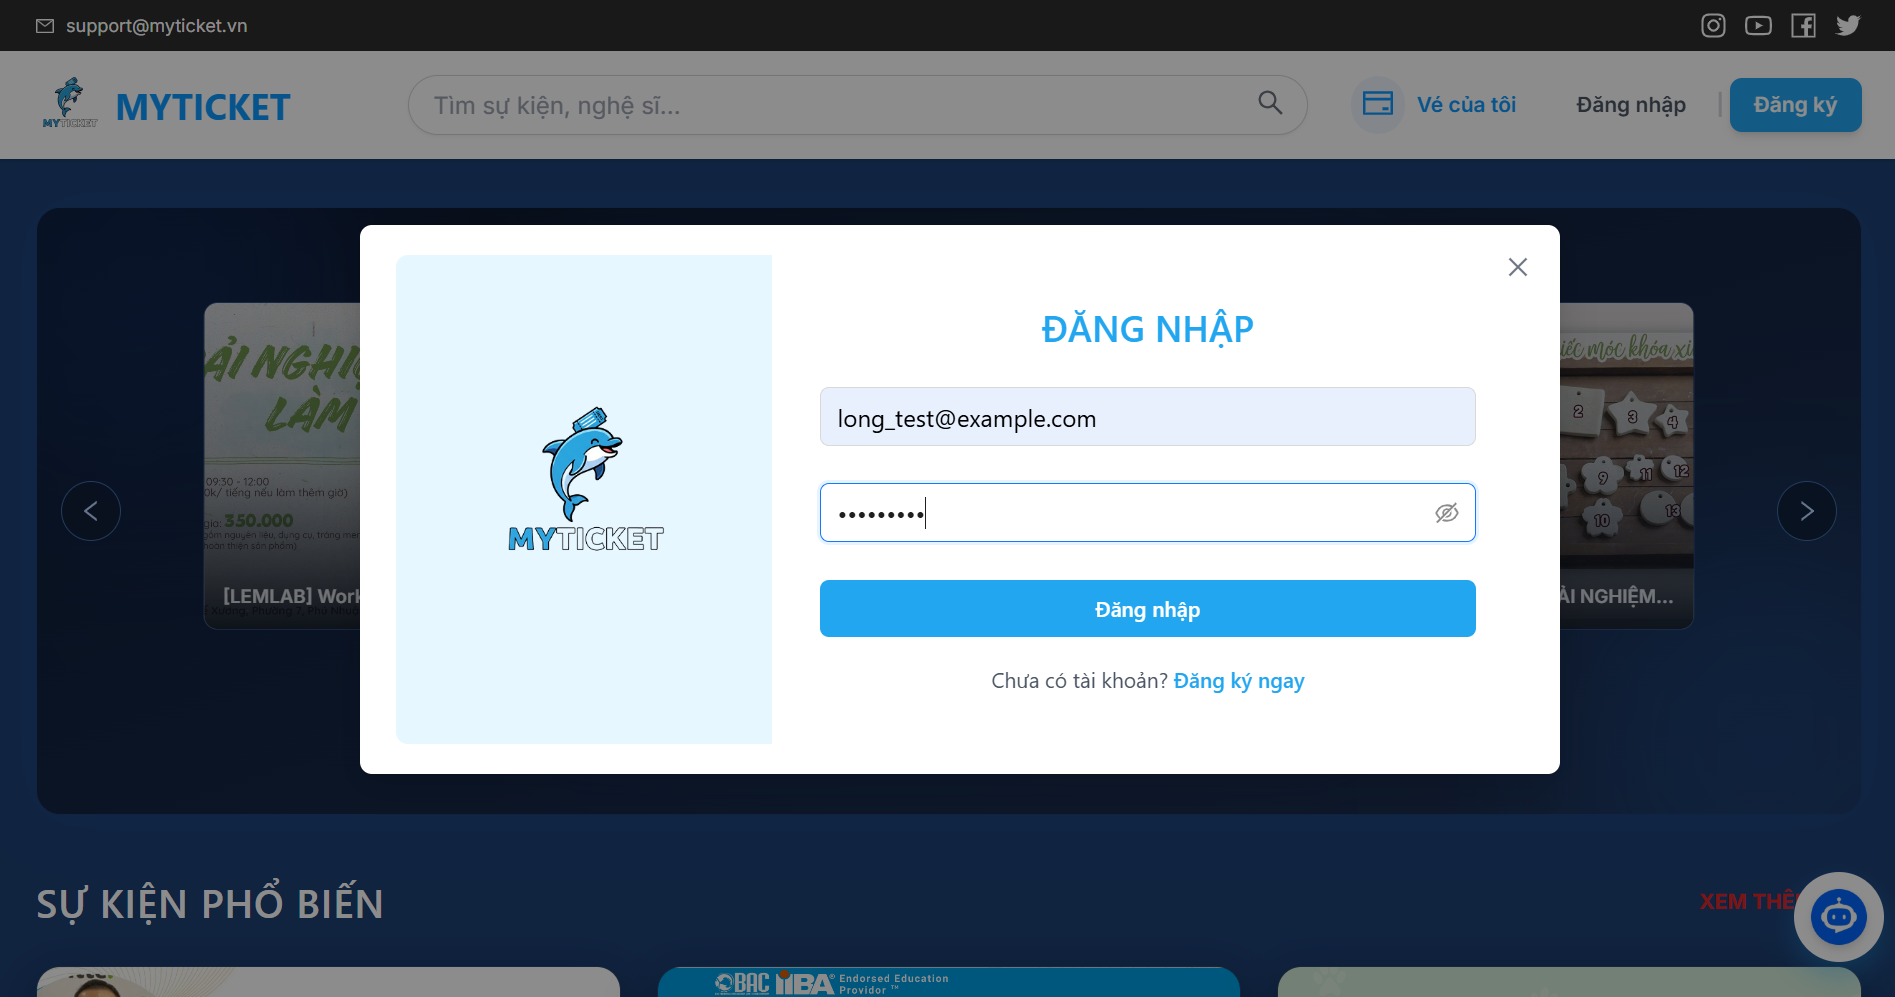
\includegraphics[width=0.65\textwidth]{Contents/UI/QTV/QTV DN.png}
    \vspace{15pt}
    \caption{Giao diện quản trị viên nhập thông tin đăng nhập}
\end{figure}
\begin{figure}[H]
    \centering
    
\includegraphics[width=0.65\textwidth]{Contents/UI/QTV/QTV DN TC.png}
    \vspace{15pt}
    \caption{Giao diện quản trị viên sau khi đăng nhập thành công}
\end{figure}
\indent Tại đây, Quản trị viên có thể thực hiện các nhóm chức năng chính được mô tả chi tiết ở các phần tiếp theo.

\subsubsection{Trang dữ liệu thống kê}
\begin{figure}[H]
    \centering
    
\includegraphics[width=0.65\textwidth]{Contents/UI/QTV/DL TK.png}
    \vspace{15pt}
    \caption{Giao diện hiển thị dữ liệu thống kê của Quản trị viên}
\end{figure}
\indent \indent \textbf{Mô tả:}\\
\indent - Khi đăng nhập thành công với role Admin, hệ thống sẽ tự động điều hướng giao diện sang trang này. Ngoài ra, Quản trị viên cũng có thể nhấn vào mục "Statistical Data" ở thanh navbar để truy cập vào trang này.\\
\indent - Tại đây, Quản trị viên có thể xem được các dữ liệu thống kê tổng quan bao gồm: số lượng sự kiện, tổng số đơn vị tổ chức sự kiện hay sự thay đổi gần đây về sự kiện mới trong tháng, khách hàng đăng ký mới, ban tổ chức mới kèm dấu hiệu tăng/giảm/ổn định.\\


\subsubsection{Quản lý thông tin sự kiện}
\begin{figure}[H]
    \centering
    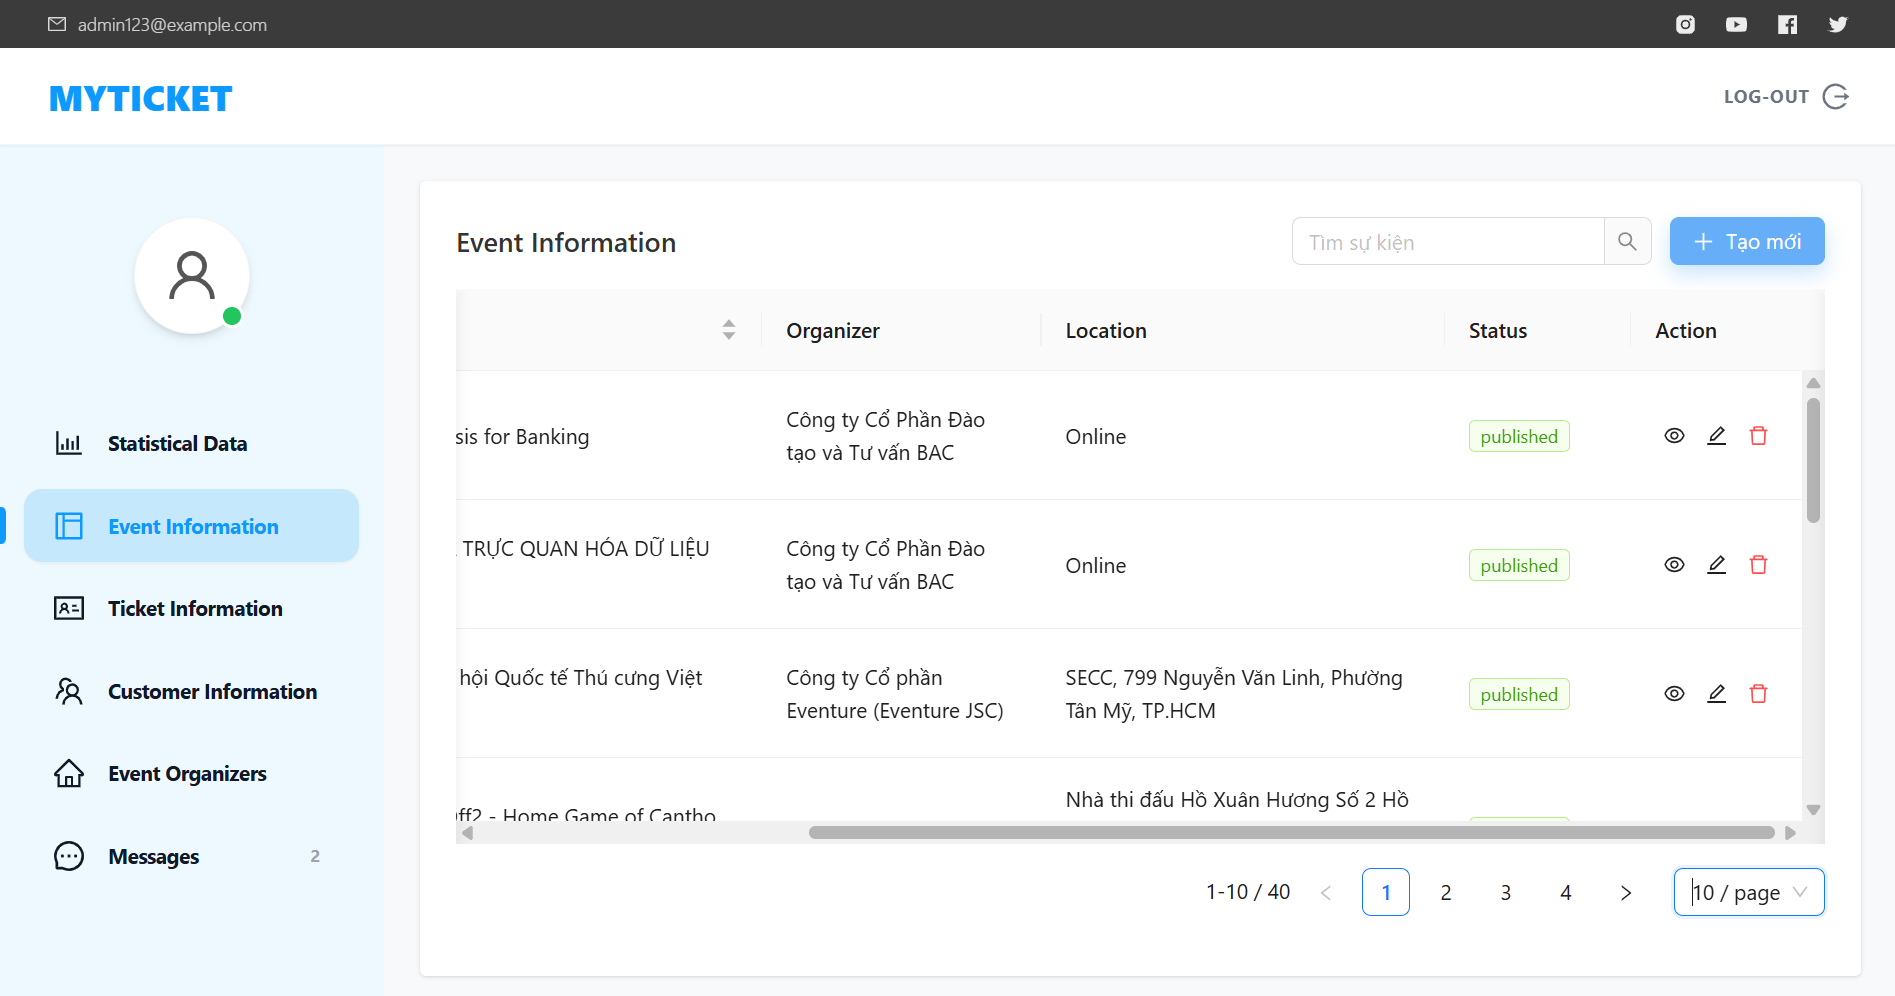
\includegraphics[width=0.65\textwidth]{Contents/UI/QTV/event infor.png}
    \vspace{15pt}
    \caption{Giao diện quản lý thông tin sự kiện của Quản trị viên}
\end{figure}
\indent \indent \textbf{Mô tả}:\\
\indent - Tại trang này, Quản trị viên có toàn quyền xem thông tin chi tiết các sự kiện được đăng tải trên hệ thống bằng các thao tác tiện ích như:
\begin{itemize}
    \item[+] Nhập từ khóa tìm kiếm vào thanh tìm kiếm để tìm kiếm sự kiện. Khi nhập từ khóa tìm kiếm tới đâu thì hệ thống sẽ ngay lập tức hiển thị kết quả phù hợp tới đó.
    \begin{figure}[H]
        \centering
        
\includegraphics[width=0.65\textwidth]{Contents/UI/QTV/search event.png}
        \vspace{15pt}
        \caption{Giao diện hiển thị kết quả tìm kiếm sự kiện tại trang quản lý thông tin sự kiện của Quản trị viên}
    \end{figure}
    \item[+] Cuộn dọc hoặc cuộn ngang để xem thông tin của các sự kiện.
    \item[+] Chọn sự kiện muốn hiện thị trên một trang bằng cách nhấn vào nút ở góc phải màn hình với các lựa chọn 10, 20, 24, 50 hay 100 sự kiện.
    \item[+] Quan sát dãy số ở góc dưới bên phải để nắm được số lượng trang. Để chuyển trang thì cần nhấn vào số tương ứng.
\end{itemize}
\indent - Các icon ở cột action của mỗi sự kiện cho phép Quản trị viên thực hiện các chức năng sau khi nhấn vào:
\begin{itemize}
    \item[1.] \textbf{Icon eye:} Hiển thị thông tin chi tiết của của một sự kiện đã chọn.
    \begin{figure}[H]
        \centering
        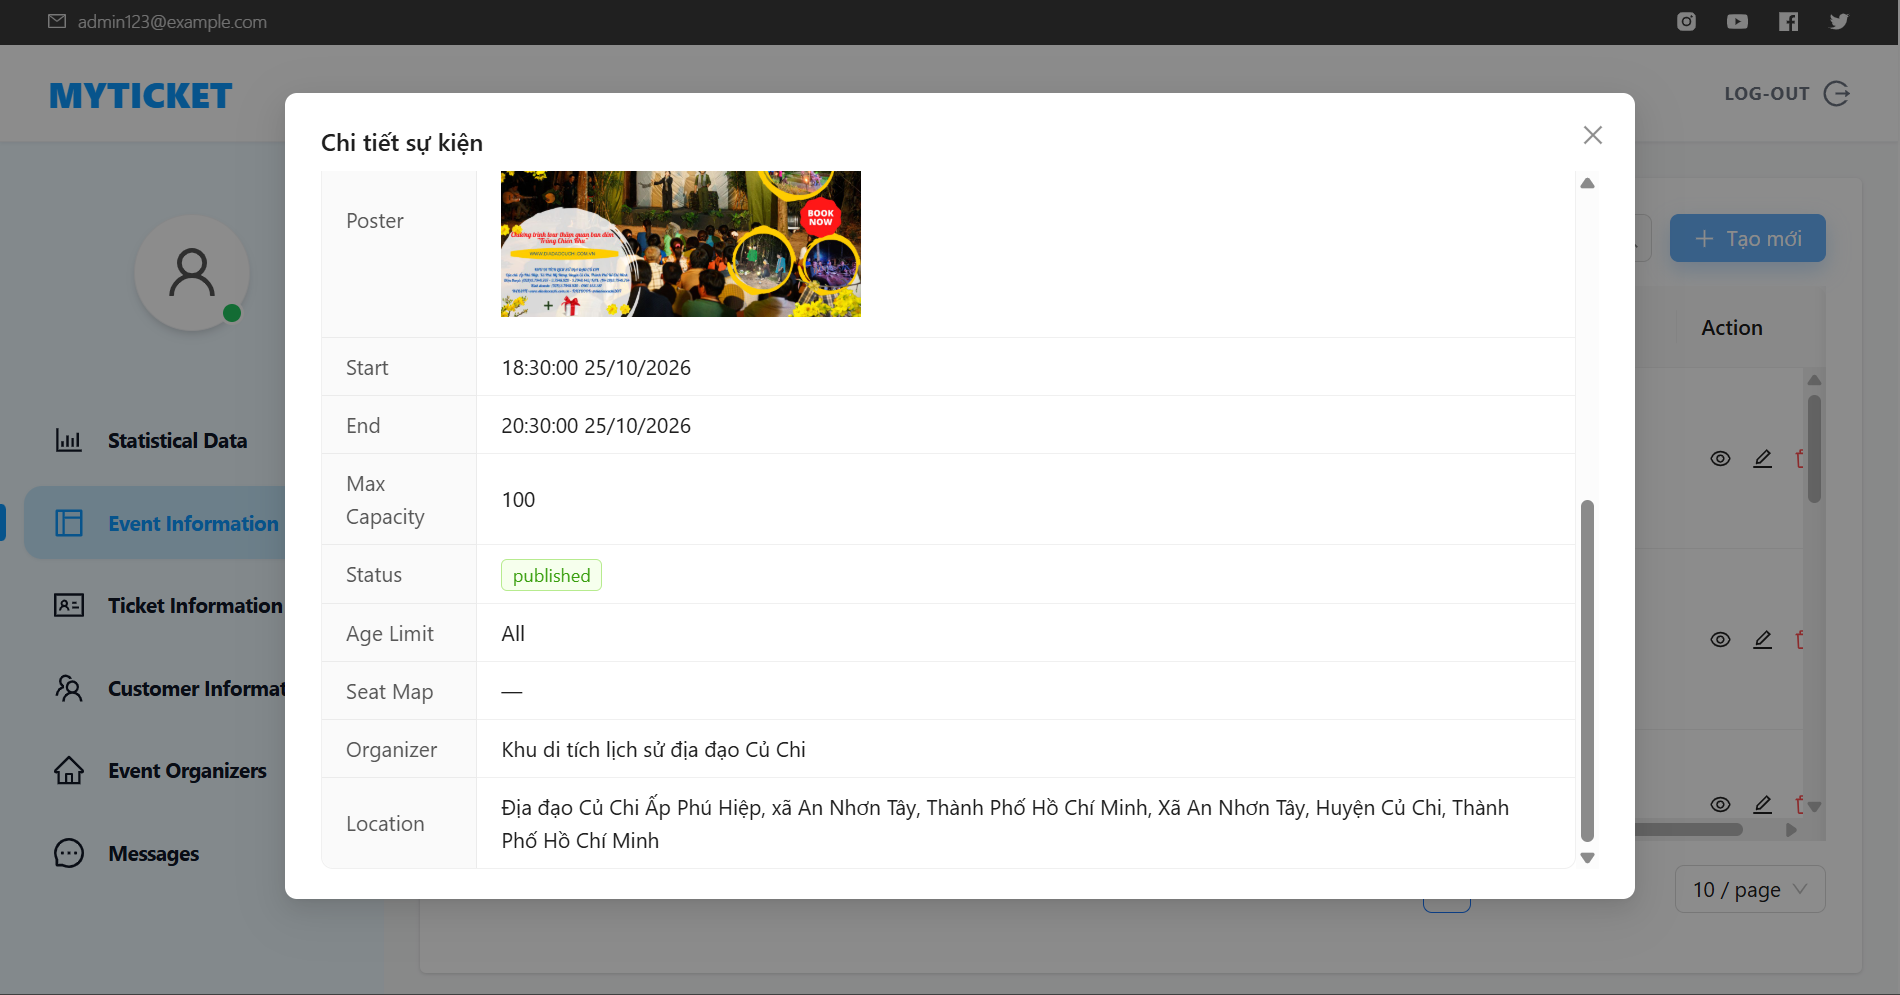
\includegraphics[width=0.65\textwidth]{Contents/UI/QTV/view selected event.png}
        \vspace{15pt}
        \caption{Giao diện hiển thị chi tiết thông tin một sự kiện cụ thể tại trang quản lý thông tin của Quản trị viên}
    \end{figure}
    \item[2.] \textbf{Icon pencil:} Chỉnh sửa thông tin của một sự kiện đã chọn.
    \begin{figure}[H]
        \centering
        
\includegraphics[width=0.65\textwidth]{Contents/UI/QTV/edit selected event.png}
        \vspace{15pt}
        \caption{Giao diện chỉnh sửa thông tin một sự kiện cụ thể tại trang quản lý thông tin của Quản trị viên}
    \end{figure}
    \item[3.] \textbf{Icon trash:} Xóa một sự kiện đã chọn.
    \begin{figure}[H]
        \centering
        
\includegraphics[width=0.65\textwidth]{Contents/UI/QTV/delete selected event.png}
        \vspace{15pt}
        \caption{Giao diện xác nhận xóa một sự kiện cụ thể tại trang quản lý thông tin của Quản trị viên}
    \end{figure}
\end{itemize}
\indent - Để tạo mới sự kiện, Quản trị viên cần nhấn vào nút "+ Tạo mới" ở góc phải trên. Trước khi tạo thông tin sự kiện, bắt buộc phải có thông tin về ban tổ chức.
\begin{figure}[H]
    \centering
    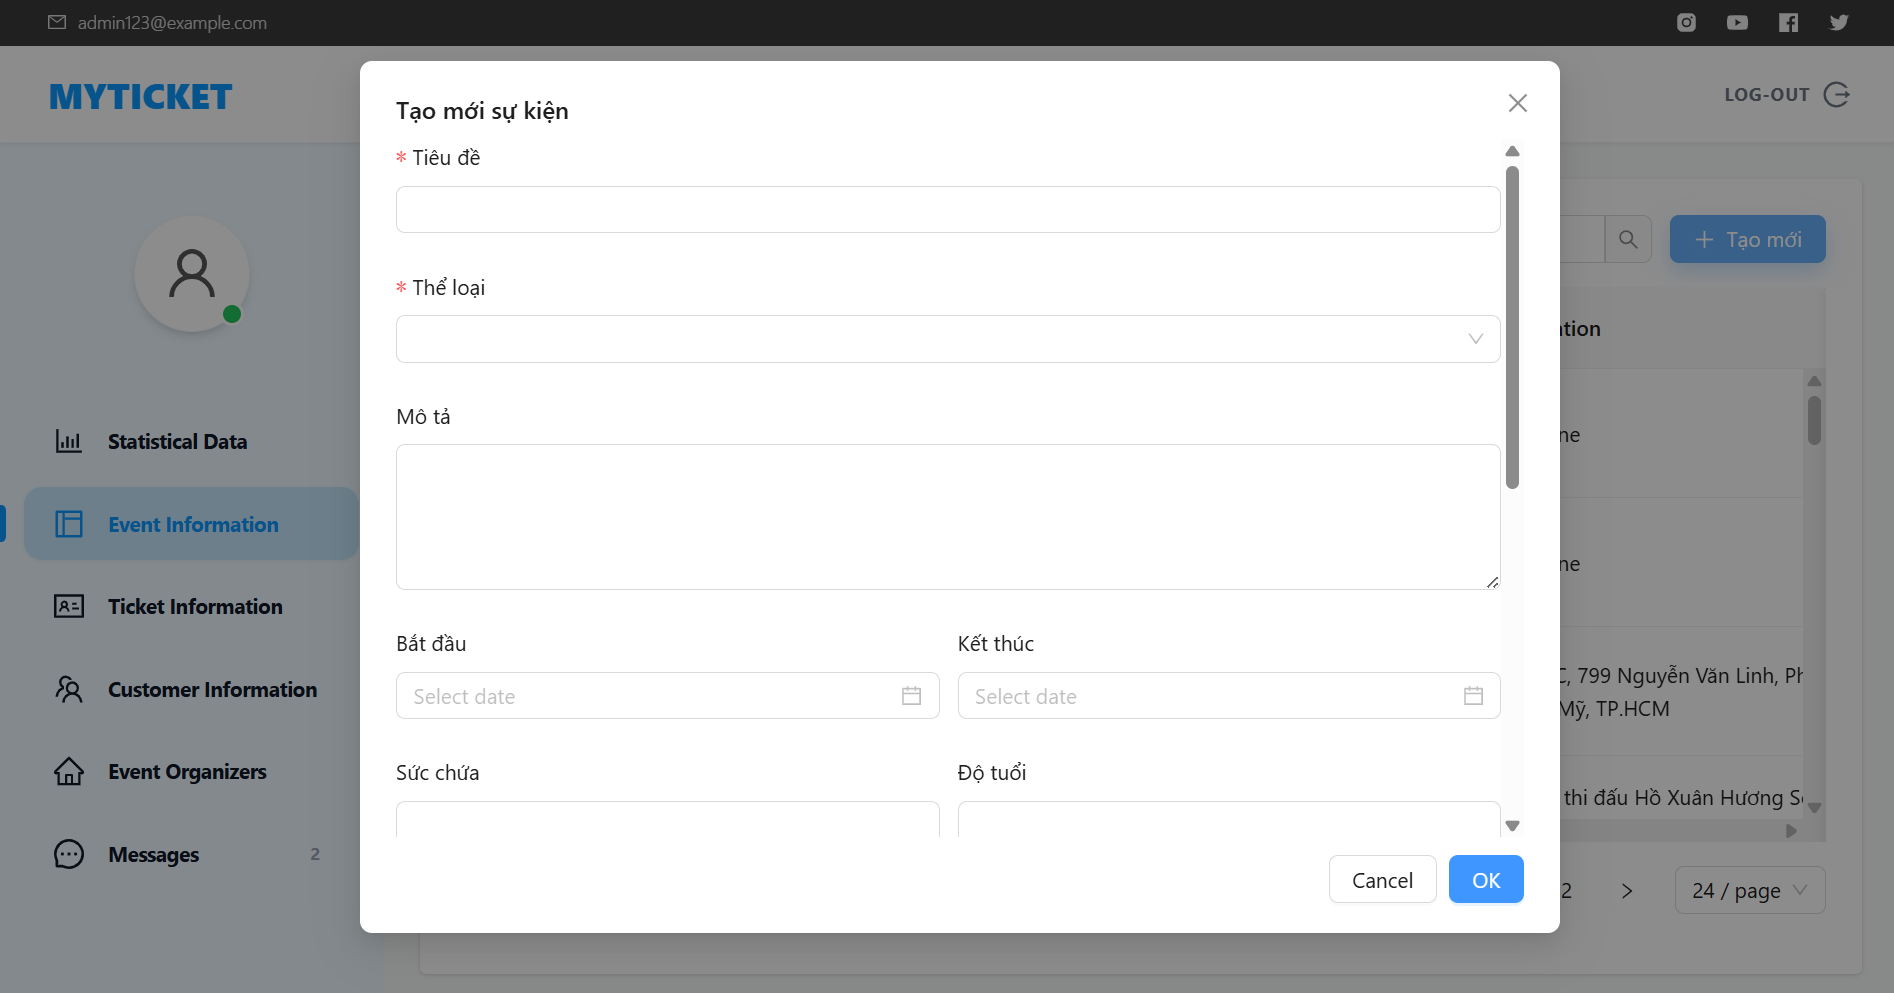
\includegraphics[width=0.65\textwidth]{Contents/UI/QTV/create new event.png}
    \vspace{15pt}
    \caption{Giao diện tạo mới sự kiện tại trang quản lý thông tin sự kiện của Quản trị viên}
\end{figure}

\subsubsection{Quản lý thông tin Ban tổ chức}
\begin{figure}[H]
    \centering
    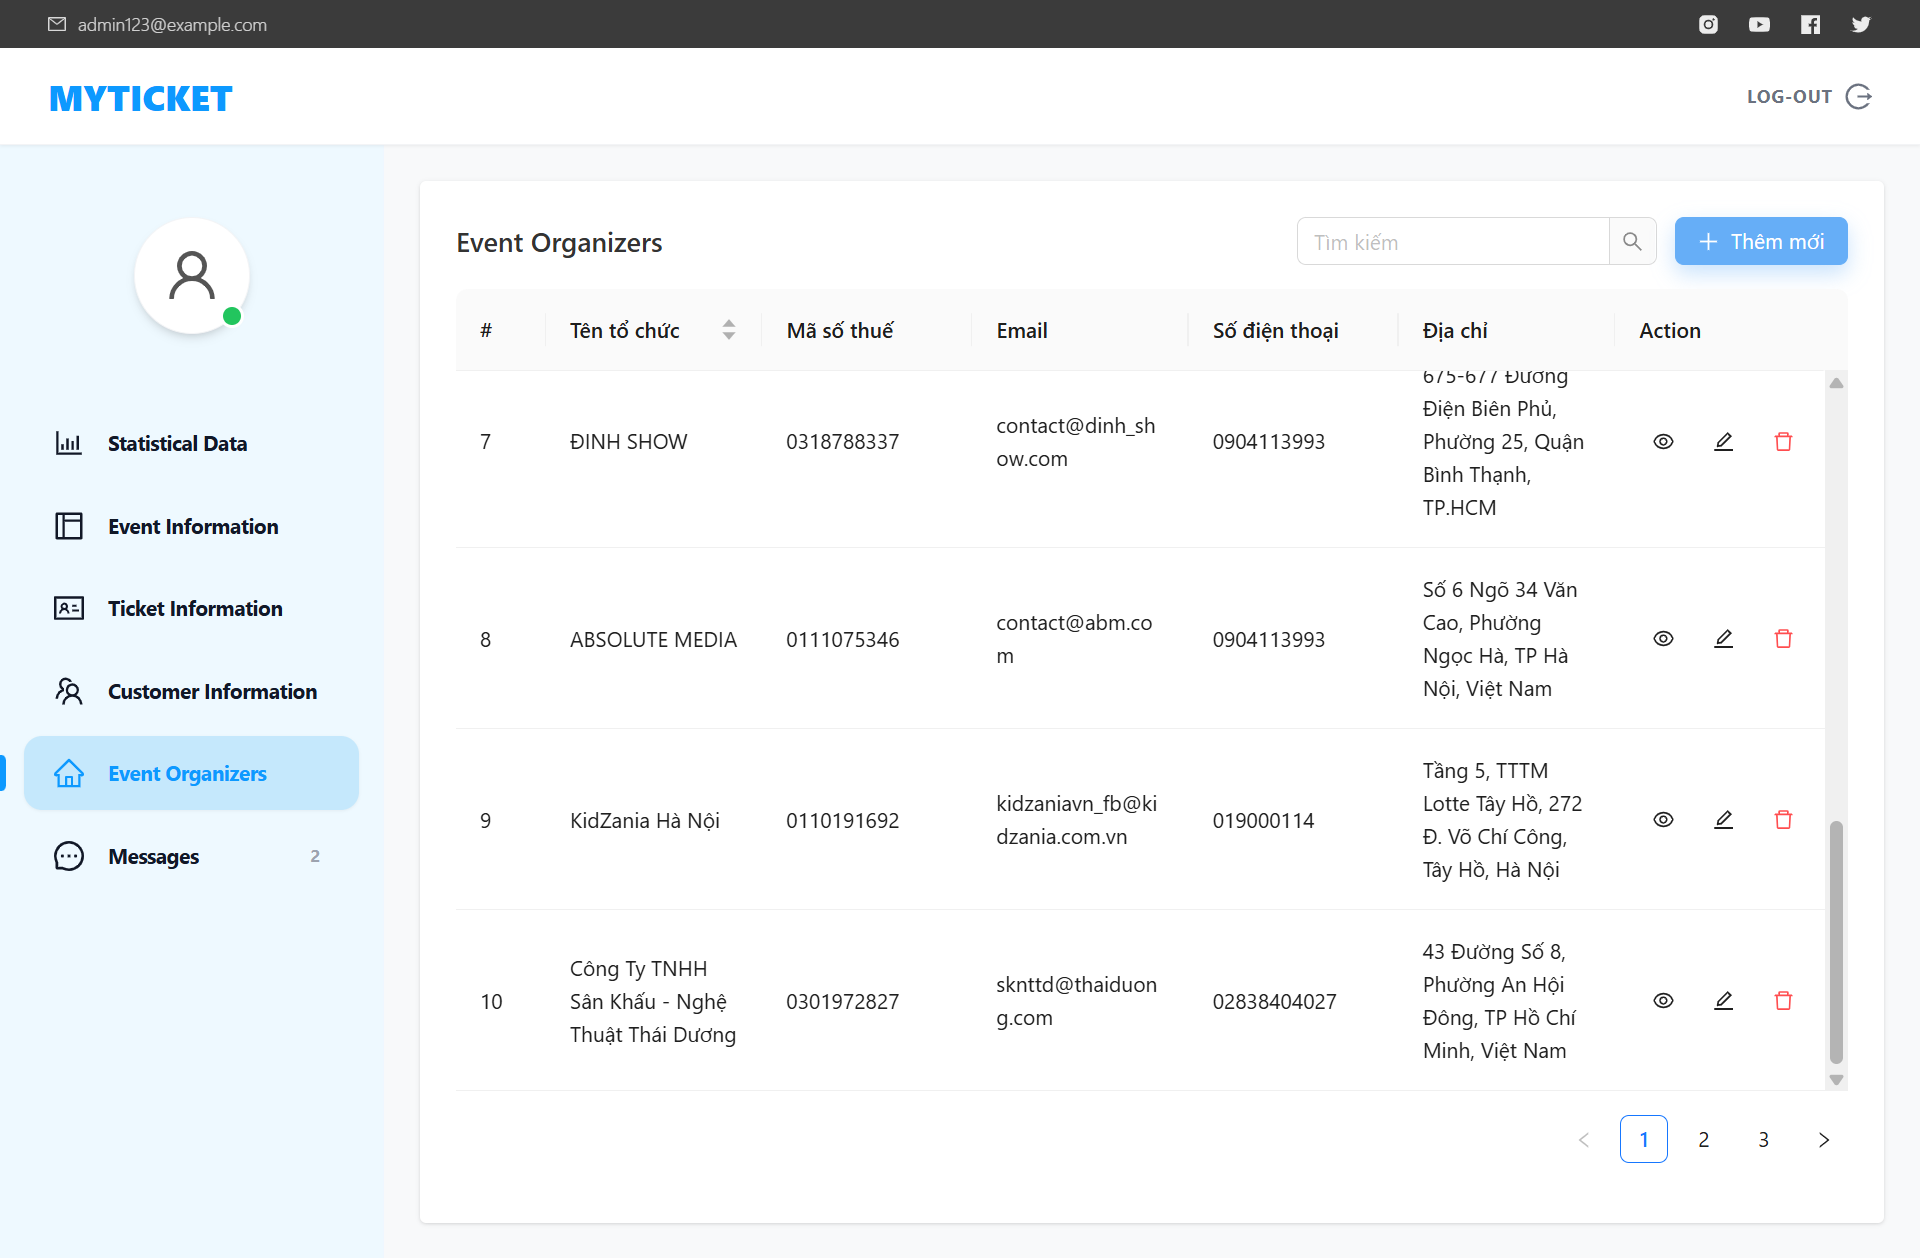
\includegraphics[width=0.65\textwidth]{Contents/UI/QTV/tt btc.png}
    \vspace{15pt}
    \caption{Giao diện quản lý thông tin Ban tổ chức của Quản trị viên}
\end{figure}
\indent \indent \textbf{Mô tả:} \\
\indent - Quản trị viên cần nhấn vào mục "Event Organizers" ở thanh navbar để truy cập vào trang này.\\
\indent - Quản trị viên có thể tìm kiếm, cuộn dọc hoặc cuộn ngang để xem thông tin của các Ban tổ chức. Để chuyển trang, cần nhấn nút ô chứ số trang tương ứng hoặc các mũi tên điều hướng ở góc phải dưới.
\begin{figure}
    \centering
    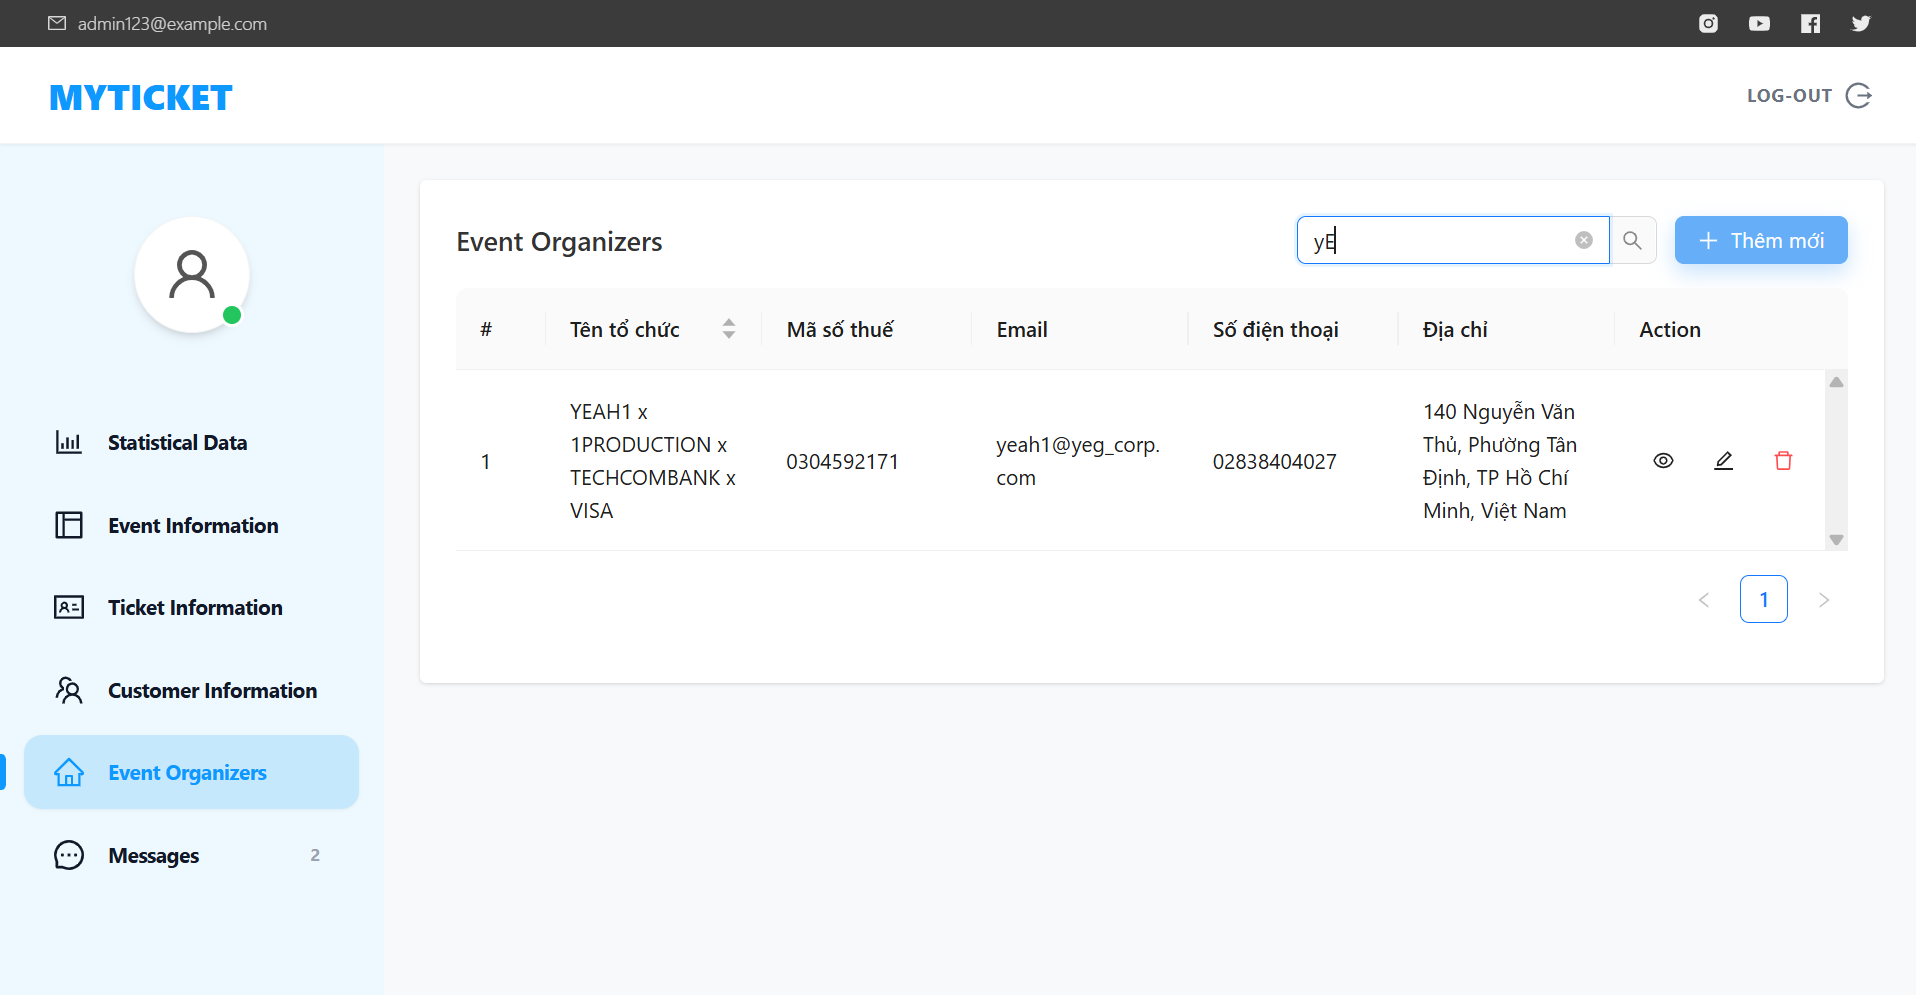
\includegraphics[width=0.65\textwidth]{Contents/UI/QTV/search btc.png}
    \vspace{15pt}
    \caption{Giao diện hiển thị kết quả tìm kiếm Ban tổ chức tại trang quản lý thông tin Ban tổ chức của Quản trị viên}
\end{figure}
\indent - Tại trang này, Quản trị viên có toàn quyền xem, chỉnh sửa hoặc xóa thông tin của một Ban tổ chức cụ thể bằng cách nhấn vào các icon tương ứng ở cột action:
\begin{itemize}
    \item[1.] \textbf{Icon eye:} Hiển thị thông tin chi tiết của một Ban tổ chức đã chọn.
    \begin{figure}[H]
        \centering
        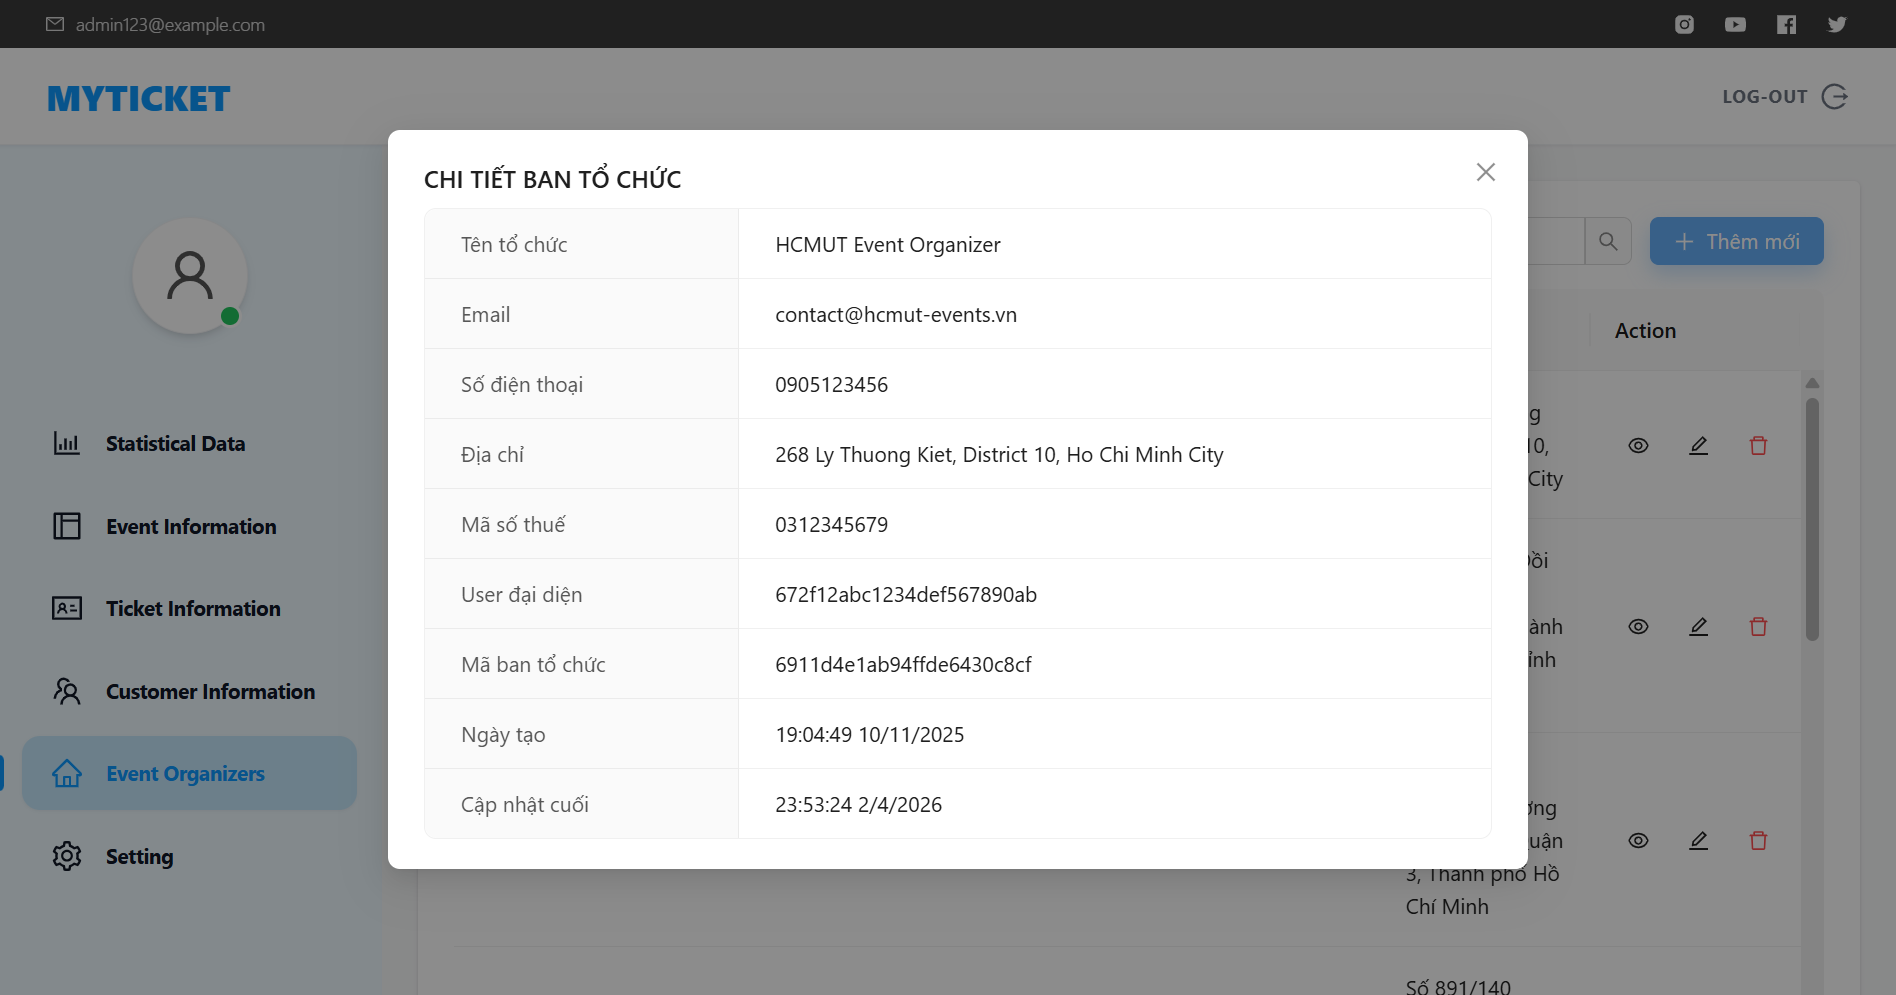
\includegraphics[width=0.65\textwidth]{Contents/UI/QTV/detail infor btc.png}
        \vspace{15pt}
        \caption{Giao diện hiển thị chi tiết thông tin một Ban tổ chức cụ thể tại trang quản lý thông tin Ban tổ chức của Quản trị viên}
    \end{figure}
    \item[2.] \textbf{Icon pencil:} Chỉnh sửa thông tin của một Ban tổ chức đã chọn.
    \begin{figure}[H]
        \centering
        
\includegraphics[width=0.65\textwidth]{Contents/UI/QTV/edit btc.png}
        \vspace{15pt}
        \caption{Giao diện chỉnh sửa thông tin một Ban tổ chức cụ thể tại trang quản lý thông tin Ban tổ chức của Quản trị viên}
    \end{figure}
    \item[3.] \textbf{Icon trash:} Xóa một Ban tổ chức đã chọn.
    \begin{figure}[H]
        \centering
        
\includegraphics[width=0.65\textwidth]{Contents/UI/QTV/delete btc.png}
        \vspace{15pt}
        \caption{Giao diện xác nhận xóa một Ban tổ chức cụ thể tại trang quản lý thông tin Ban tổ chức của Quản trị viên}
    \end{figure}
\end{itemize}
\indent - Để tạo mới Ban tổ chức, Quản trị viên cần nhấn vào nút "+ Tạo mới" ở góc phải trên. Sau đó, điền đầy đủ thông tin ở các trường theo đúng format quy định để tạo mới Ban tổ chức thành công.
\begin{figure}[H]
    \centering
    
\includegraphics[width=0.65\textwidth]{Contents/UI/QTV/create new btc.png}
    \vspace{15pt}
    \caption{Giao diện tạo mới Ban tổ chức tại trang quản lý thông tin Ban tổ chức của Quản trị viên}
\end{figure}


\subsubsection{Quản lý thông tin vé cho sự kiện}

\indent \indent Quản trị viên cần nhấn vào mục "Ticket Information" ở thanh navbar để truy cập vào trang này.\\
\begin{figure}
    \centering
    
\includegraphics[width=0.65\textwidth]{Contents/UI/QTV/create ticket overview.png}
    \vspace{15pt}
    \caption{Giao diện quản lý thông tin vé của Quản trị viên}
\end{figure}

\indent \textbf{Các thao tác tạo vé cho sự kiện:}
\begin{itemize}
    \item[1.] \textbf{Lựa chọn sự kiện muốn tạo vé trong list các sự kiện đã được tạo thông tin trước đó.}
    \begin{figure}[H]
        \centering
        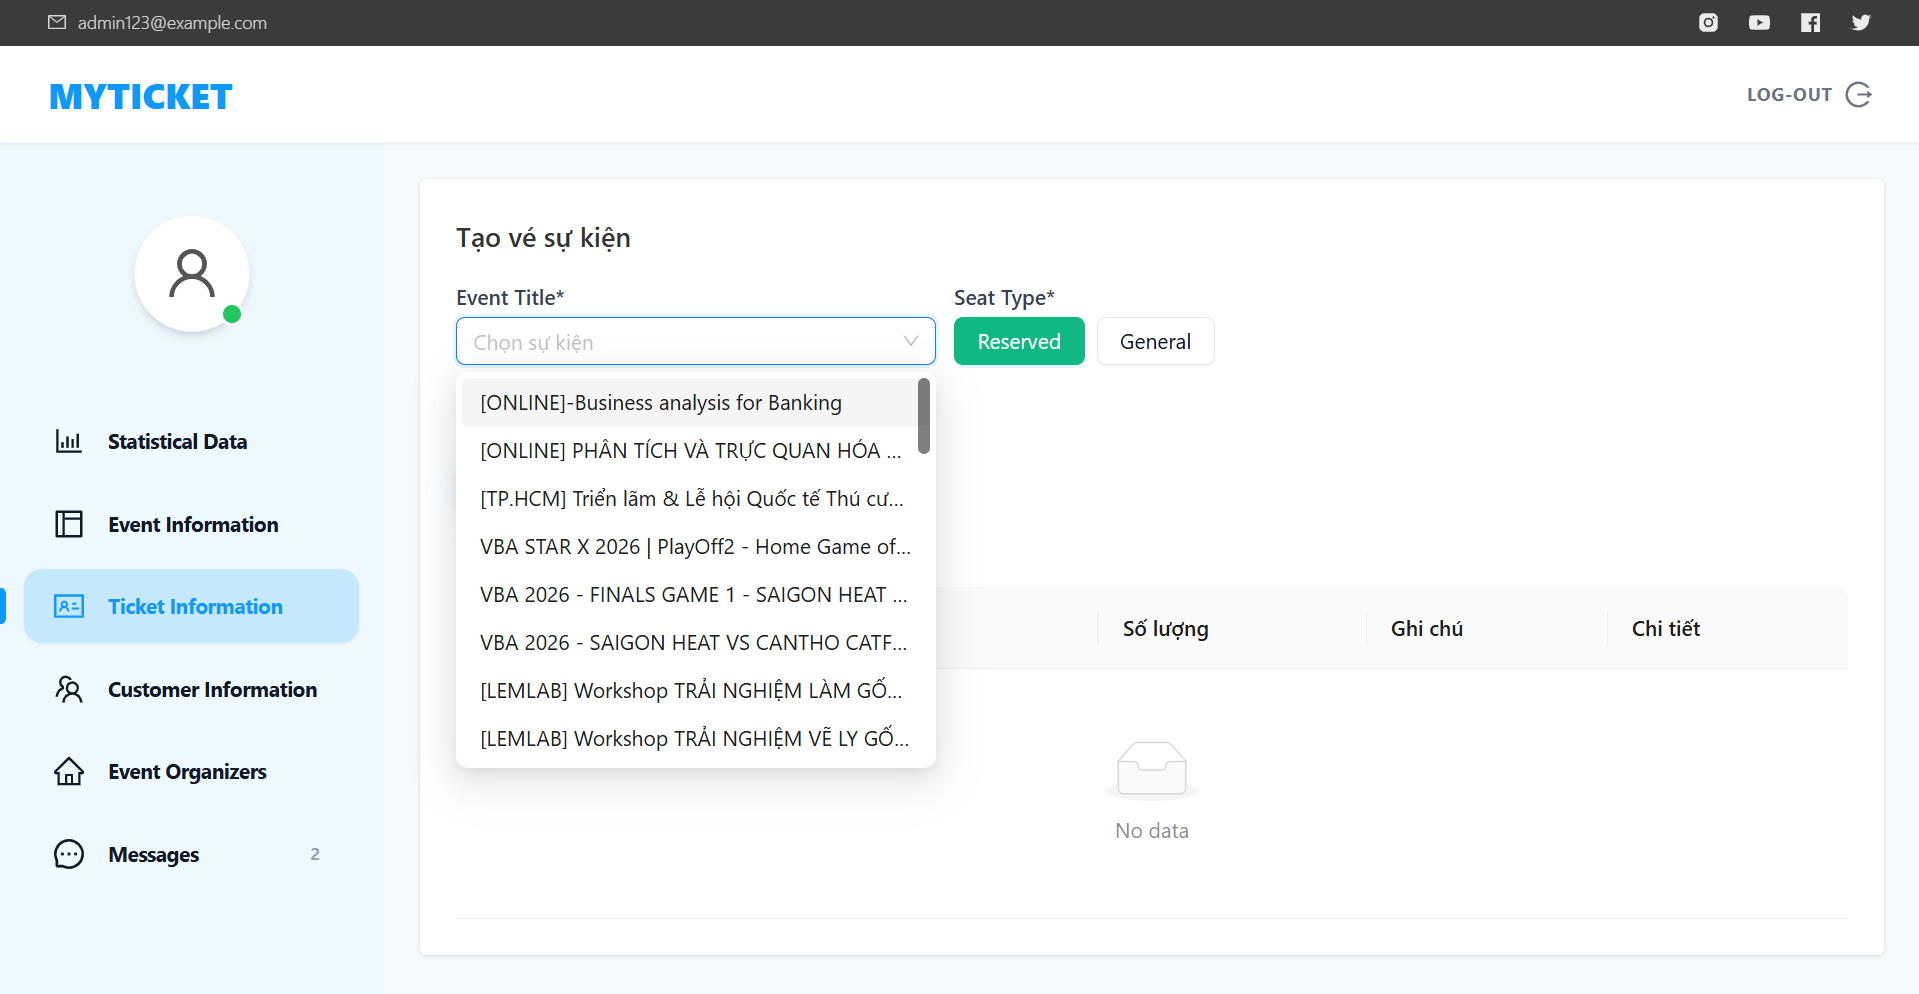
\includegraphics[width=0.65\textwidth]{Contents/UI/QTV/chọn tên sự kiện cần tạo vé.png}
        \vspace{15pt}
        \caption{Giao diện lựa chọn sự kiện để tạo vé tại trang quản lý thông tin vé của Quản trị viên}
    \end{figure}
    \item[2.] \textbf{Chọn loại vé}\\
    Sau khi chọn tên sự kiện. Quản trị viên cần chọn 1 trong 2 nút kế bên tên sự kiện để chọn loại vé: Vé có chỗ ngồi cố định (Reserved) hoặc vé có chỗ ngồi tự do (General). Sau đó nhấn vào nút "+ thêm loại vé" để điền thông vé.
    \item[3.] \textbf{Điền và lưu thông tin vé}
    \begin{itemize}
        \item[3.1] \textbf{Đối với vé có chỗ ngồi tự do (Generel)}
        \begin{figure}[H]
            \centering
            
\includegraphics[width=0.65\textwidth]{Contents/UI/QTV/điền tt vé general.png}
            \vspace{15pt}
            \caption{Giao diện điền thông tin vé có chỗ ngồi tự do tại trang quản lý thông tin vé của Quản trị viên}
        \end{figure}
        Các thông tin cần điền bao gồm: Tên vé, giá vé và số lượng. Sau khi điền xong thông tin, Quản trị viên có thể làm tiếp một trong các lựa chọn sau:
        \begin{itemize}
            \item[] \textbf{Lựa chọn 1:} Nhấn nút "Save" để lưu thông tin vé vừa điền vào bảng vé hiện có của sự kiện.
            \begin{figure}[H]
                \centering
                
\includegraphics[width=0.65\textwidth]{Contents/UI/QTV/save lưu 1 vé cho general.png}
                \vspace{15pt}
                \caption{Giao diện lưu thông tin một vé có chỗ ngồi tự do sau khi nhấn nút "Save" tại trang quản lý thông tin vé của Quản trị viên}
            \end{figure}
            \item[] \textbf{Lựa chọn 2:} Nhấn nút "Delete" để xóa thông tin vé vừa điền nếu muốn.
            \item[] \textbf{Lựa chọn 3:} Nhấn nút "+ Thêm loại vé" để tiếp tục tạo thêm vé mới cho sự kiện này với cùng loại vé là general rồi điền tiếp thông tin cho vé mới. Sau khi tạo xong 1 loạt vé thì nhấn vào nút "Save" kế bên một vé cụ thể nếu chỉ muốn thêm một mình vé đó hoặc nhấn nút "Confirm" để lưu cùng lúc tất cả vé vào bảng vé hiện có của sự kiện.
            \begin{figure}[H]
                \centering
                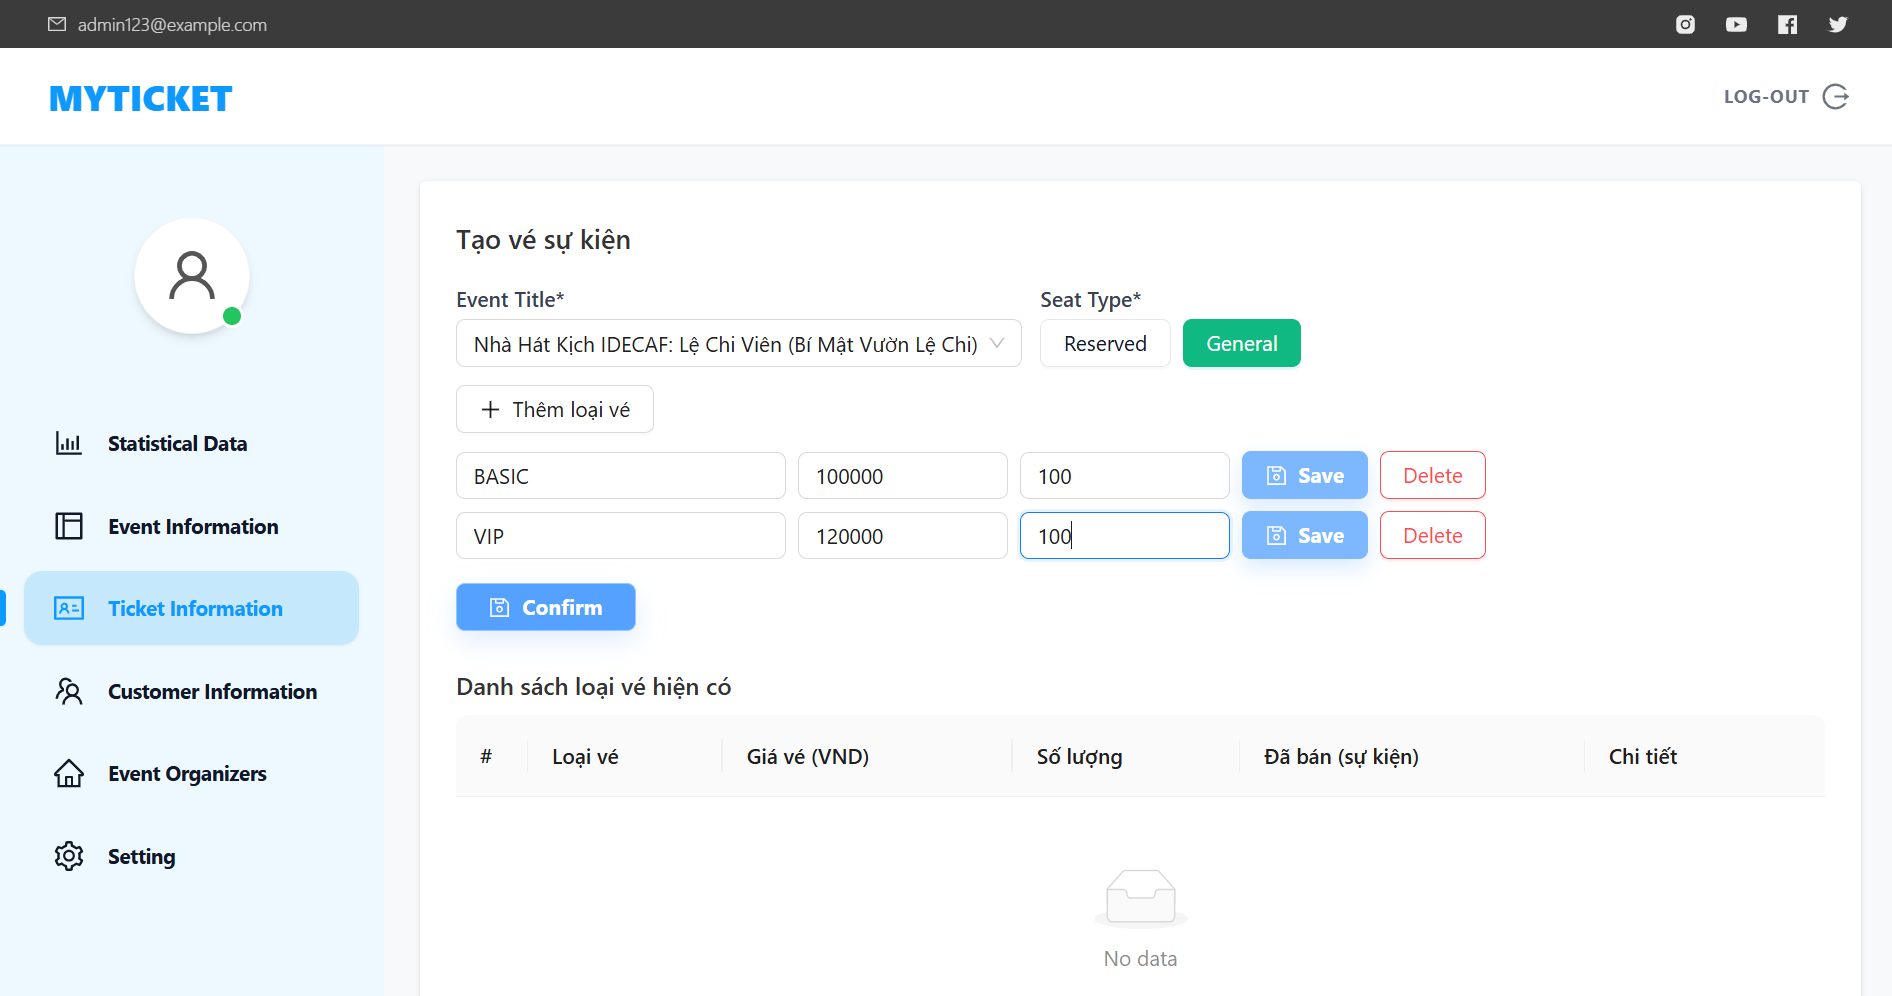
\includegraphics[width=0.65\textwidth]{Contents/UI/QTV/tạo nhiều vé general.png}
                \vspace{15pt}
                \caption{Giao diện tạo và điền thông tin nhiều vé có chỗ ngồi tự do cùng lúc tại trang quản lý thông tin vé của Quản trị viên}
            \end{figure}
            \item[] \textbf{Lựa chọn 4:} Nếu muốn tạo thêm vé mới cho sự kiện này thuộc loại vé có chỗ ngồi cố định thì thực hiện lựa chọn 1 để lưu thông tin vé trước đó rồi tiếp tục thực hiện bước 2 để chọn loại vé là reserved rồi điền thông tin cho vé mới.
        \end{itemize}

        \item[3.2] \textbf{Đối với vé có chỗ ngồi cố định (Reserved)}
        \begin{figure}[H]
            \centering
            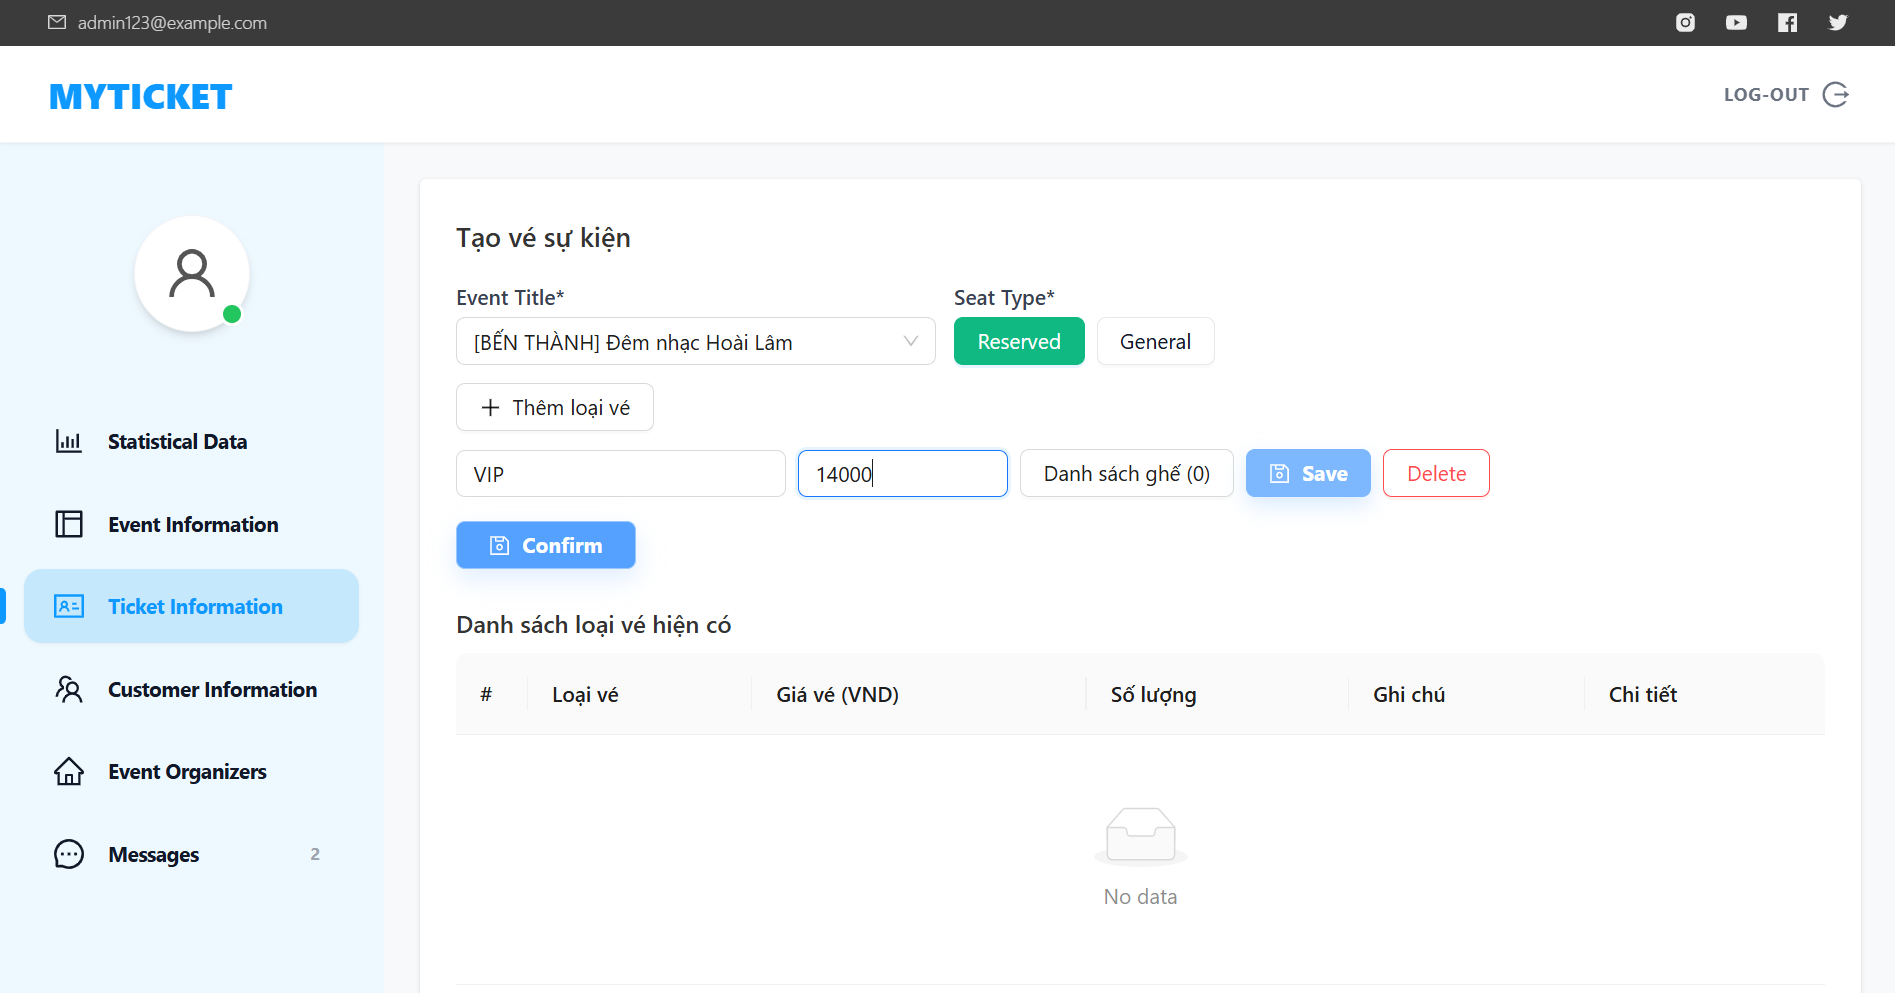
\includegraphics[width=0.65\textwidth]{Contents/UI/QTV/điền tt vé reserved.png}
            \vspace{15pt}
            \caption{Giao diện điền thông tin vé có chỗ ngồi cố định tại trang quản lý thông tin vé của Quản trị viên}
        \end{figure}
        Các thông tin cần điền bao gồm: Tên vé và giá vé. Sau đó chọn nút "Danh sách ghế" để điền thông tin ghế.
        \begin{figure}[H]
            \centering
            
\includegraphics[width=0.65\textwidth]{Contents/UI/QTV/điền ds ghế.png}
            \vspace{15pt}
            \caption{Giao diện điền thông tin ghế cho vé có chỗ ngồi cố định sau khi nhấn nút "Save" tại trang quản lý thông tin vé của Quản trị viên}
        \end{figure}
        Quản trị viên sẽ nhập tên rồi nhấn "Add" để thêm ghế vào danh sách. Tại đây mã ghế cũng chính là tên ghế, và nếu nhập sai thì có có thể nhấn nút "Delete" để xóa đi rồi nhập lại hoặc không thì cứ tiếp tục nhập tên rồi nhấn "Add" để tạo ghế mới.\\
        Sau khi nhập xong thông tin ghế, cần nhấn nút "OK" để lưu thông tin ghế vào vé và giao diện sẽ quay lại giao diện điền thông tin vé trước đó cùng với con số ở nút "Danh sách ghế" đã được thay đổi bằng số lượng ghế vừa điền. Lúc này Quản trị viên có thể thực hiện một trong các lựa chọn sau:
        \begin{itemize}
            \item[] \textbf{Lựa chọn 1:} Nhấn lại nút "Danh sách ghế" của vé trước đó để điền thêm thông tin ghế nếu muốn.
            \item[] \textbf{Lựa chọn 2:} Nhấn nút "Save" ở để lưu thông tin vé vừa điền vào bảng vé hiện có của sự kiện.
            \begin{figure}[H]
                \centering
                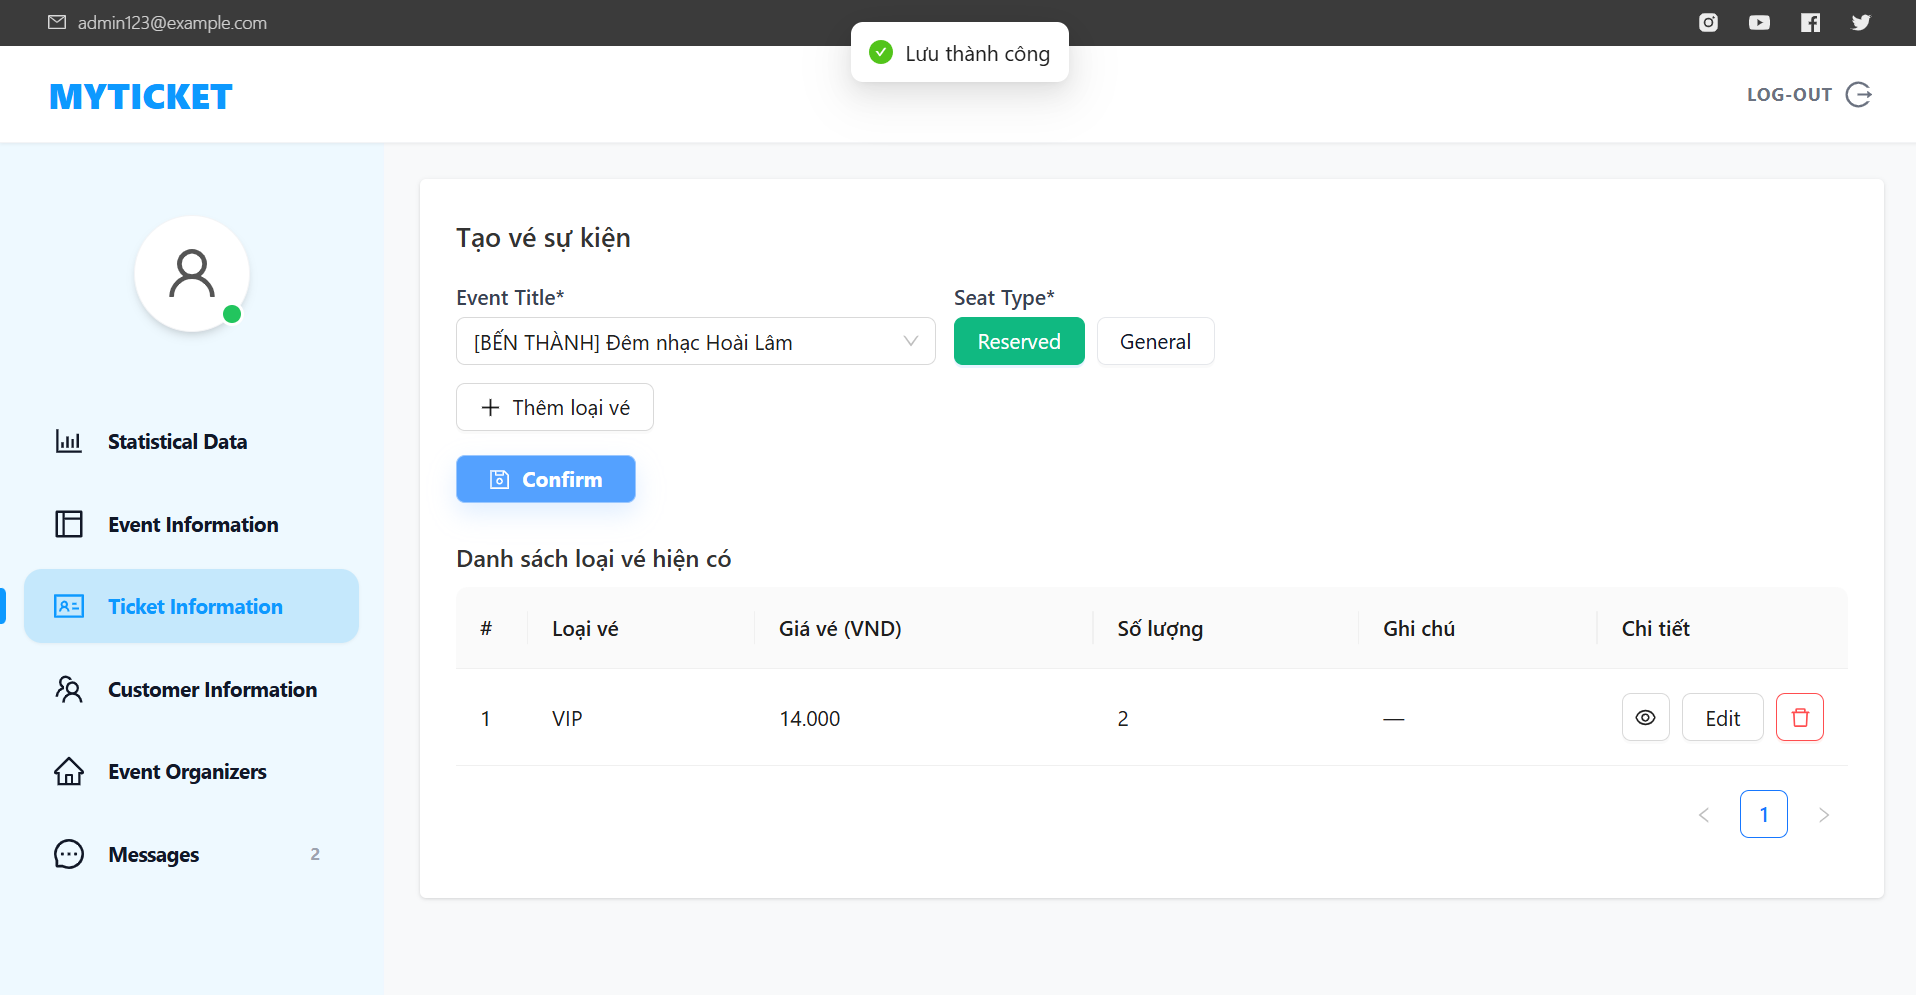
\includegraphics[width=0.65\textwidth]{Contents/UI/QTV/Lưu tt 1 vé reserved.png}
                \vspace{15pt}
                \caption{Giao diện lưu thông tin một vé có chỗ ngồi cố định tại trang quản lý thông tin vé của Quản trị viên}
            \end{figure}
            \item[] \textbf{Lựa chọn 3:} Nhấn nút "Delete" để xóa thông tin vé vừa điền nếu muốn.
            \item[] \textbf{Lựa chọn 4:} Nhấn nút "+ Thêm loại vé" để tiếp tục tạo thêm vé mới cho sự kiện này với cùng loại vé là reserved rồi điền tiếp thông tin cho vé mới. Sau khi tạo xong 1 loạt vé thì nhấn vào nút "Save" kế bên một vé cụ thể nếu chỉ muốn thêm một mình vé đó hoặc nhấn nút "Confirm" để lưu cùng lúc tất cả vé vào bảng vé hiện có của sự kiện.
            \begin{figure}[H]
                \centering
                
\includegraphics[width=0.65\textwidth]{Contents/UI/QTV/Tạo 1 loạt vé reserved.png}
                \vspace{15pt}
                \caption{Giao diện tạo và điền thông tin nhiều vé có chỗ ngồi cố định cùng lúc tại trang quản lý thông tin vé của Quản trị viên}
            \end{figure}
            \item[] \textbf{Lựa chọn 5:} Nếu muốn tạo thêm vé mới cho sự kiện này thuộc loại vé có chỗ ngồi tự do thì thực hiện lựa chọn 2 để lưu thông tin vé trước đó rồi tiếp tục thực hiện bước 2 để chọn loại vé là general rồi điền thông tin cho vé mới.
        \end{itemize}
    \end{itemize}
    \item[4.] \textbf{Tạo vé thành công}\\
    Tất cả những vé đã được điền thông tin và được nhấn Save hoặc Confirm thành công đều sẽ được lưu vào bảng vé hiện có của sự kiện. Khi đó, những vé này sẽ được dùng để hiển thị ở trang chi tiết thông tin sự kiện và người dùng có thể mua những vé này nếu còn đủ số lượng vé.
    \begin{figure}
        \centering
        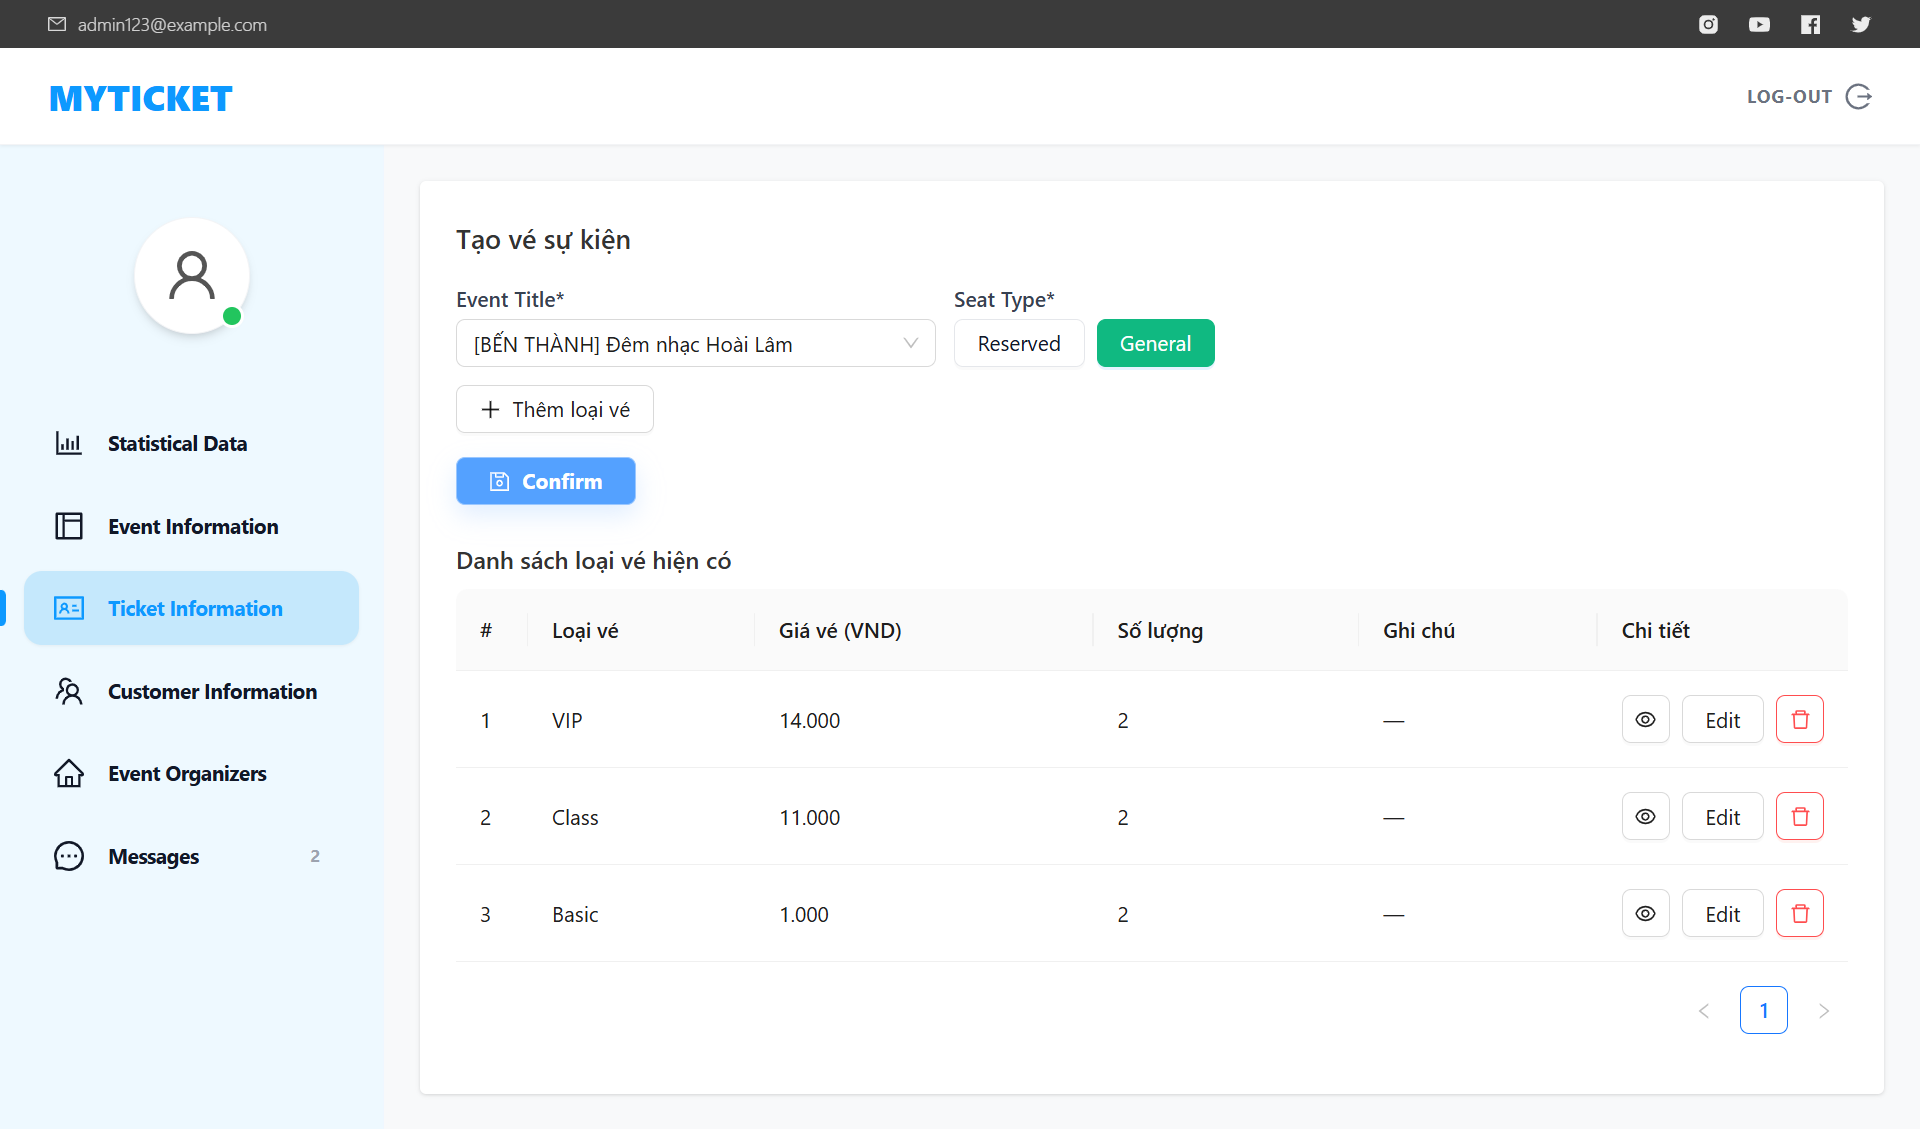
\includegraphics[width=0.65\textwidth]{Contents/UI/QTV/Giao diện bảng vé hiện có.png}
        \vspace{15pt}
        \caption{Giao diện hiển thị vé đã được lưu vào bảng vé hiện có của sự kiện tại trang quản lý thông tin vé của Quản trị viên}
    \end{figure}
\end{itemize}

\indent Để tiện cho thao tác quản lý vé, Quản trị viên cũng có thể thực hiện thêm các chức năng sau đối với những vé đã được thêm vào bảng vé hiện có tạo cột chi tiết của bảng vé:
\begin{itemize}
    \item[-] \textbf{Icon eye}: xem lại thông tin vé như Tên vé, giá và và số lượng. Nếu vé có chỗ ngồi cố định thì sẽ có thêm thông tin về danh sách ghế kèm theo.
    \begin{figure}[H]
        \centering
        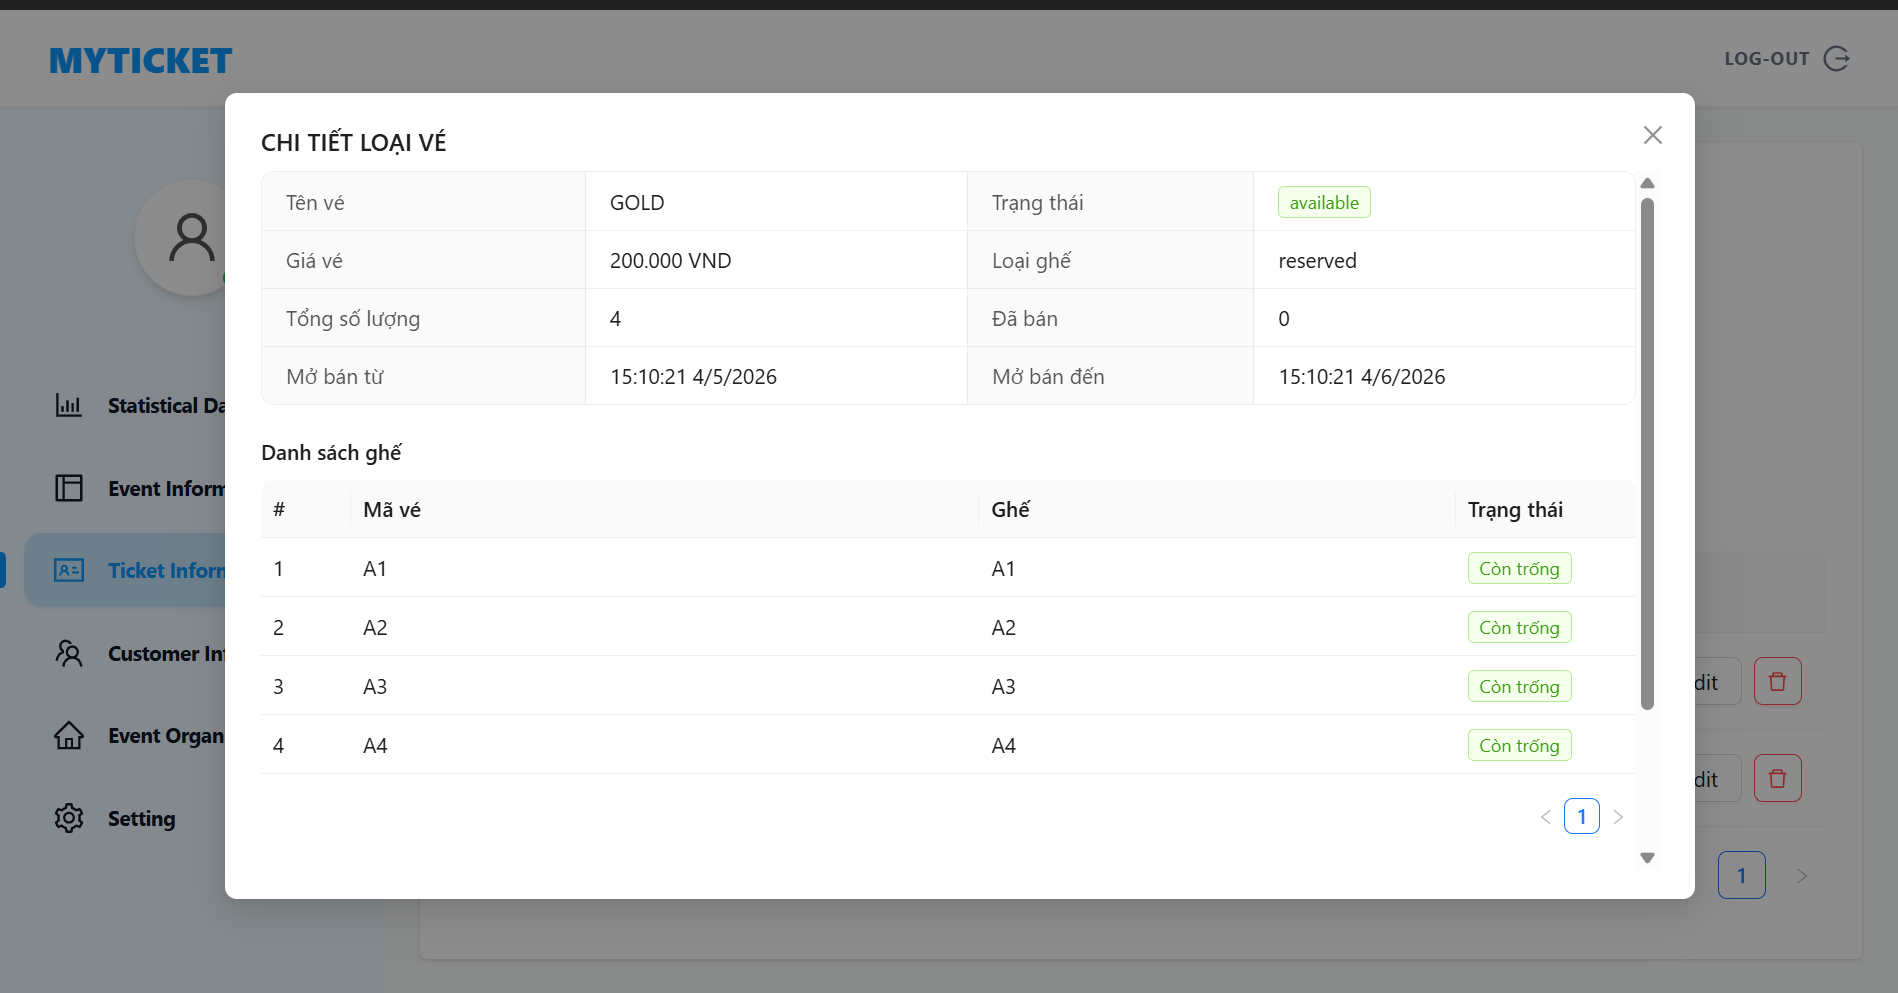
\includegraphics[width=0.65\textwidth]{Contents/UI/QTV/chi tiết loại vé.png}
        \vspace{15pt}
        \caption{Giao diện hiển thị chi tiết thông tin một vé cụ thể tại trang quản lý thông tin vé của Quản trị viên}
    \end{figure}
    \item[-] \textbf{Icon pencil}: chỉnh sửa thông tin vé. Sau khi nhấn vào icon này, giao diện sẽ hiển thị lại các trường thông tin của vé để Quản trị viên có thể chỉnh sửa. Nếu vé có chỗ ngồi cố định thì sẽ có thêm nút "Danh sách ghế" để chỉnh sửa thông tin ghế.
    \begin{figure}[H]
        \centering
        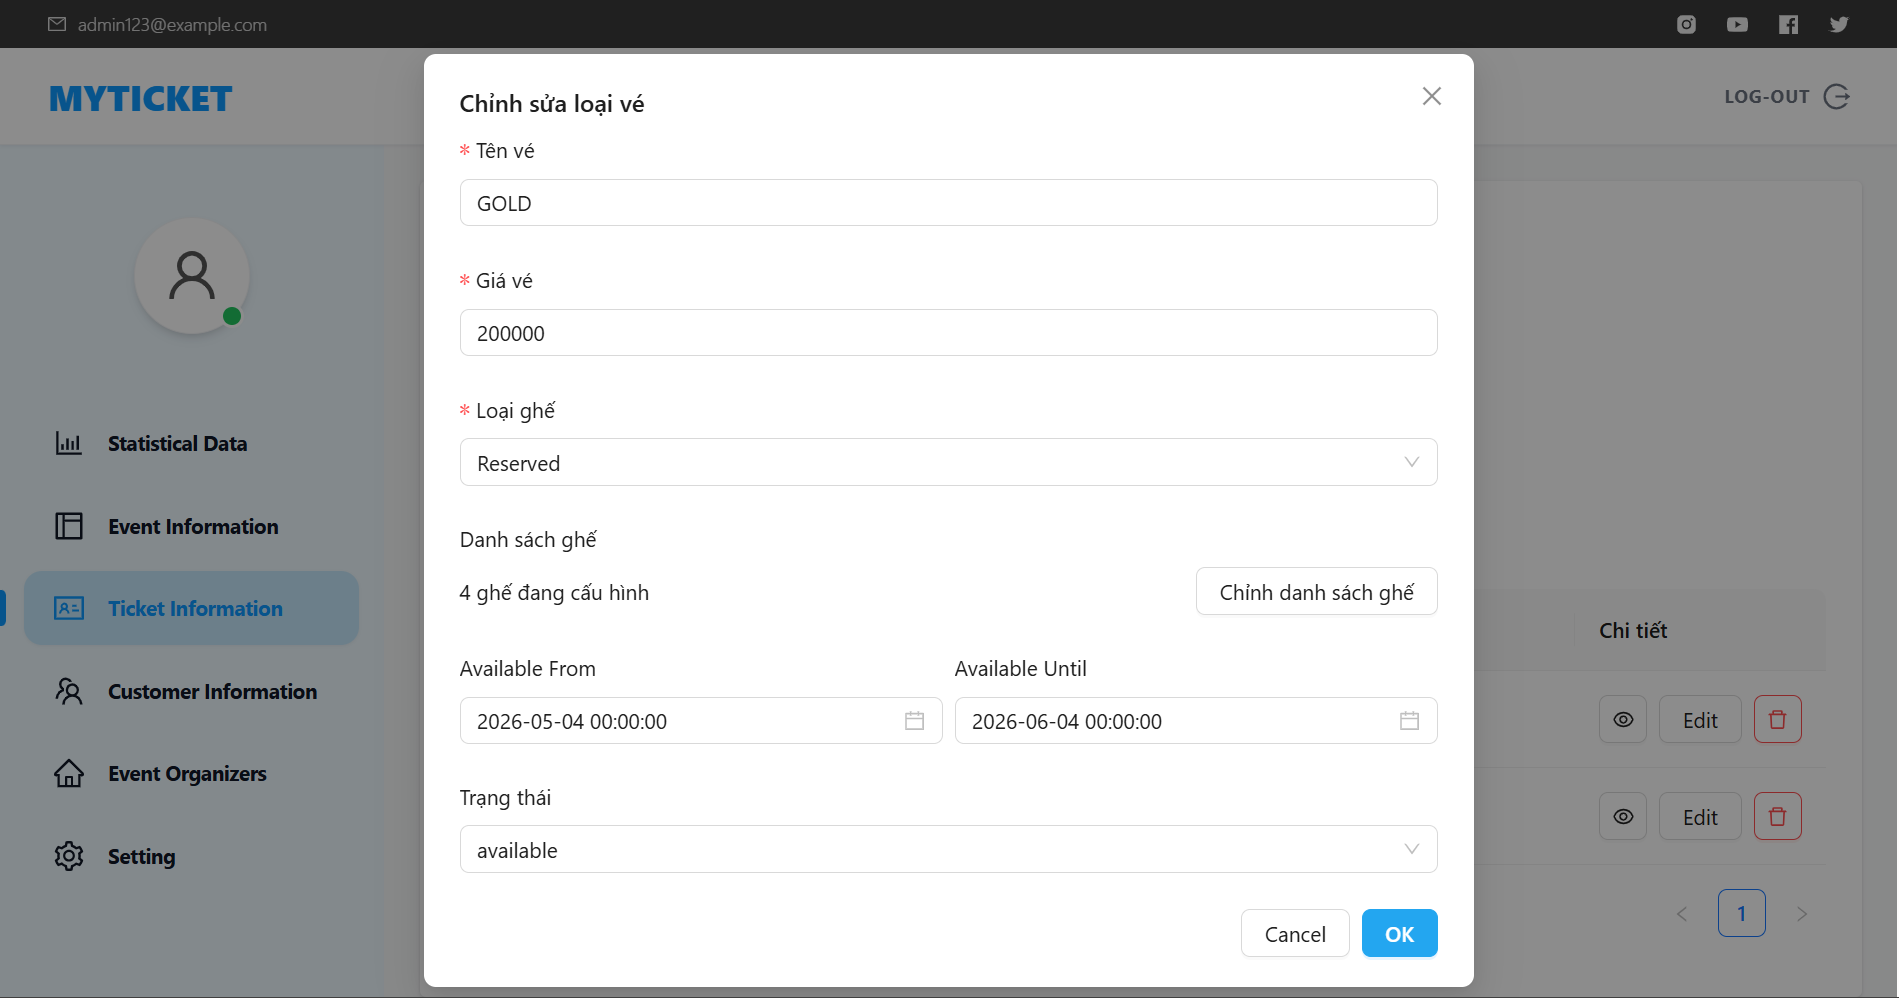
\includegraphics[width=0.65\textwidth]{Contents/UI/QTV/chỉnh sửa vé.png}
        \vspace{15pt}
        \caption{Giao diện chỉnh sửa thông tin một vé đã được lưu vào bảng vé hiện có của sự kiện tại trang quản lý thông tin vé của Quản trị viên}
    \end{figure}
    \item[-] \textbf{Icon trash}: xóa vé khỏi bảng vé hiện có của sự kiện. Khi nhấn vào icon này, hệ thống sẽ hiển thị một pop up để xác nhận việc xóa vé. Nếu Quản trị viên chọn "OK" thì vé sẽ bị xóa khỏi bảng vé hiện có của sự kiện và ngược lại nếu chọn "Cancel" thì vé sẽ không bị xóa.
\end{itemize}

\subsubsection{Quản lý thông tin người dùng}
\begin{figure}[H]
    \centering
    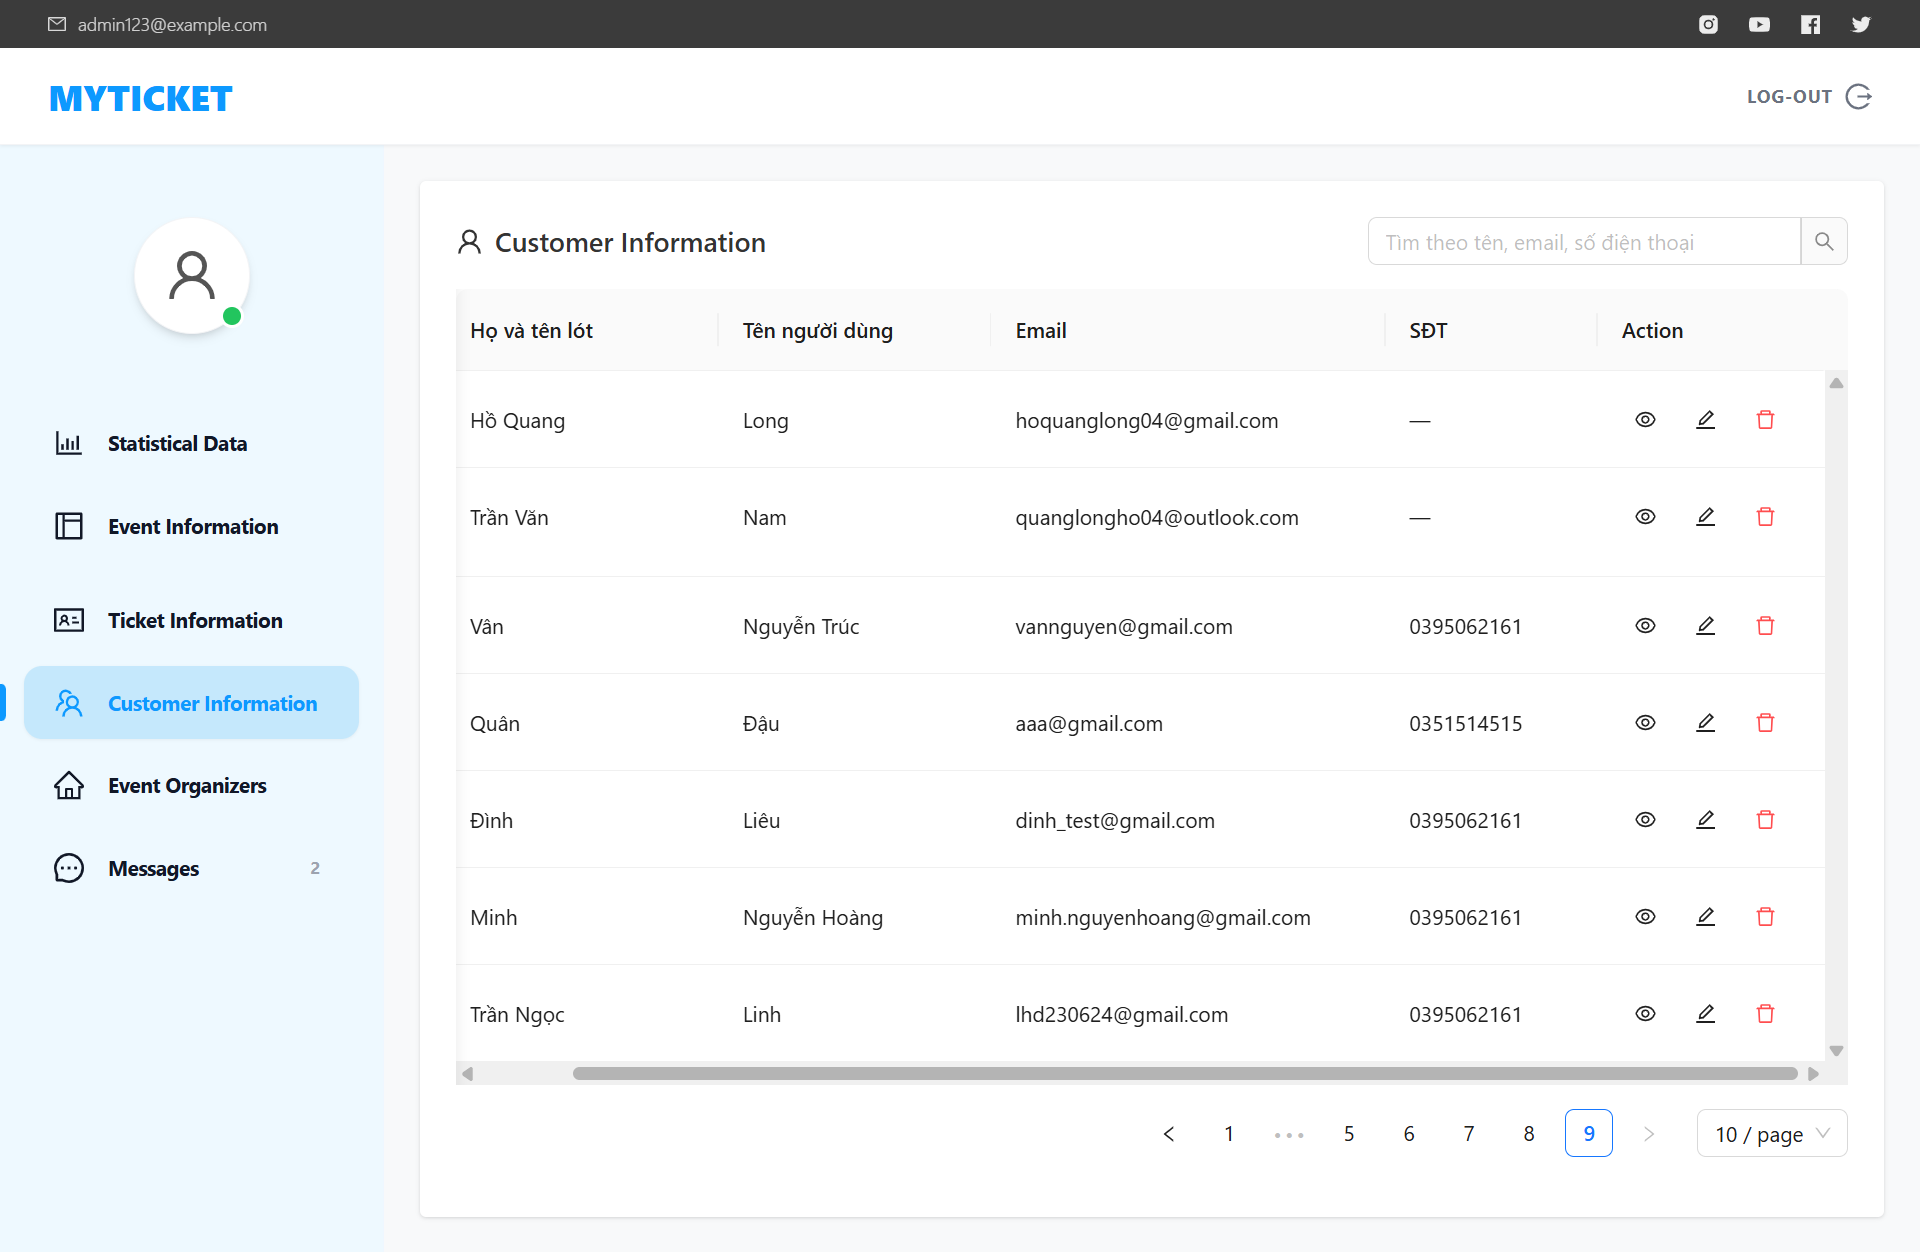
\includegraphics[width=0.65\textwidth]{Contents/UI/QTV/Quản lý TT KH.png}
    \vspace{15pt}
    \caption{Giao diện quản lý thông tin người dùng của Quản trị viên}
\end{figure}
\indent \indent \textbf{Mô tả:} \\
\indent - Quản trị viên cần nhấn vào mục "Users" ở thanh navbar để truy cập vào trang này.\\
\indent - Quản trị viên có thể tìm kiếm, cuộn dọc hoặc cuộn ngang để xem thông tin của các người dùng. Để chuyển trang, cần nhấn nút ô chứ số trang tương ứng hoặc các mũi tên điều hướng ở góc phải dưới.
\begin{figure}
    \centering
    
\includegraphics[width=0.65\textwidth]{Contents/UI/QTV/search user.png}
    \vspace{15pt}
    \caption{Giao diện hiển thị kết quả tìm kiếm người dùng tại trang quản lý thông tin người dùng của Quản trị viên}
\end{figure}
\indent - Tại trang này, Quản trị viên có toàn quyền xem, chỉnh sửa hoặc xóa thông tin của một người dùng cụ thể bằng cách nhấn vào các icon tương ứng ở cột action:
\begin{itemize}
    \item[1.] \textbf{Icon eye:} Hiển thị thông tin chi tiết của một người dùng đã chọn. Riêng cột "Trạng thái" cho biết người dùng có đang online hay không: Active (đang online) hay Inactive (đang offline).
    \begin{figure}[H]
        \centering
        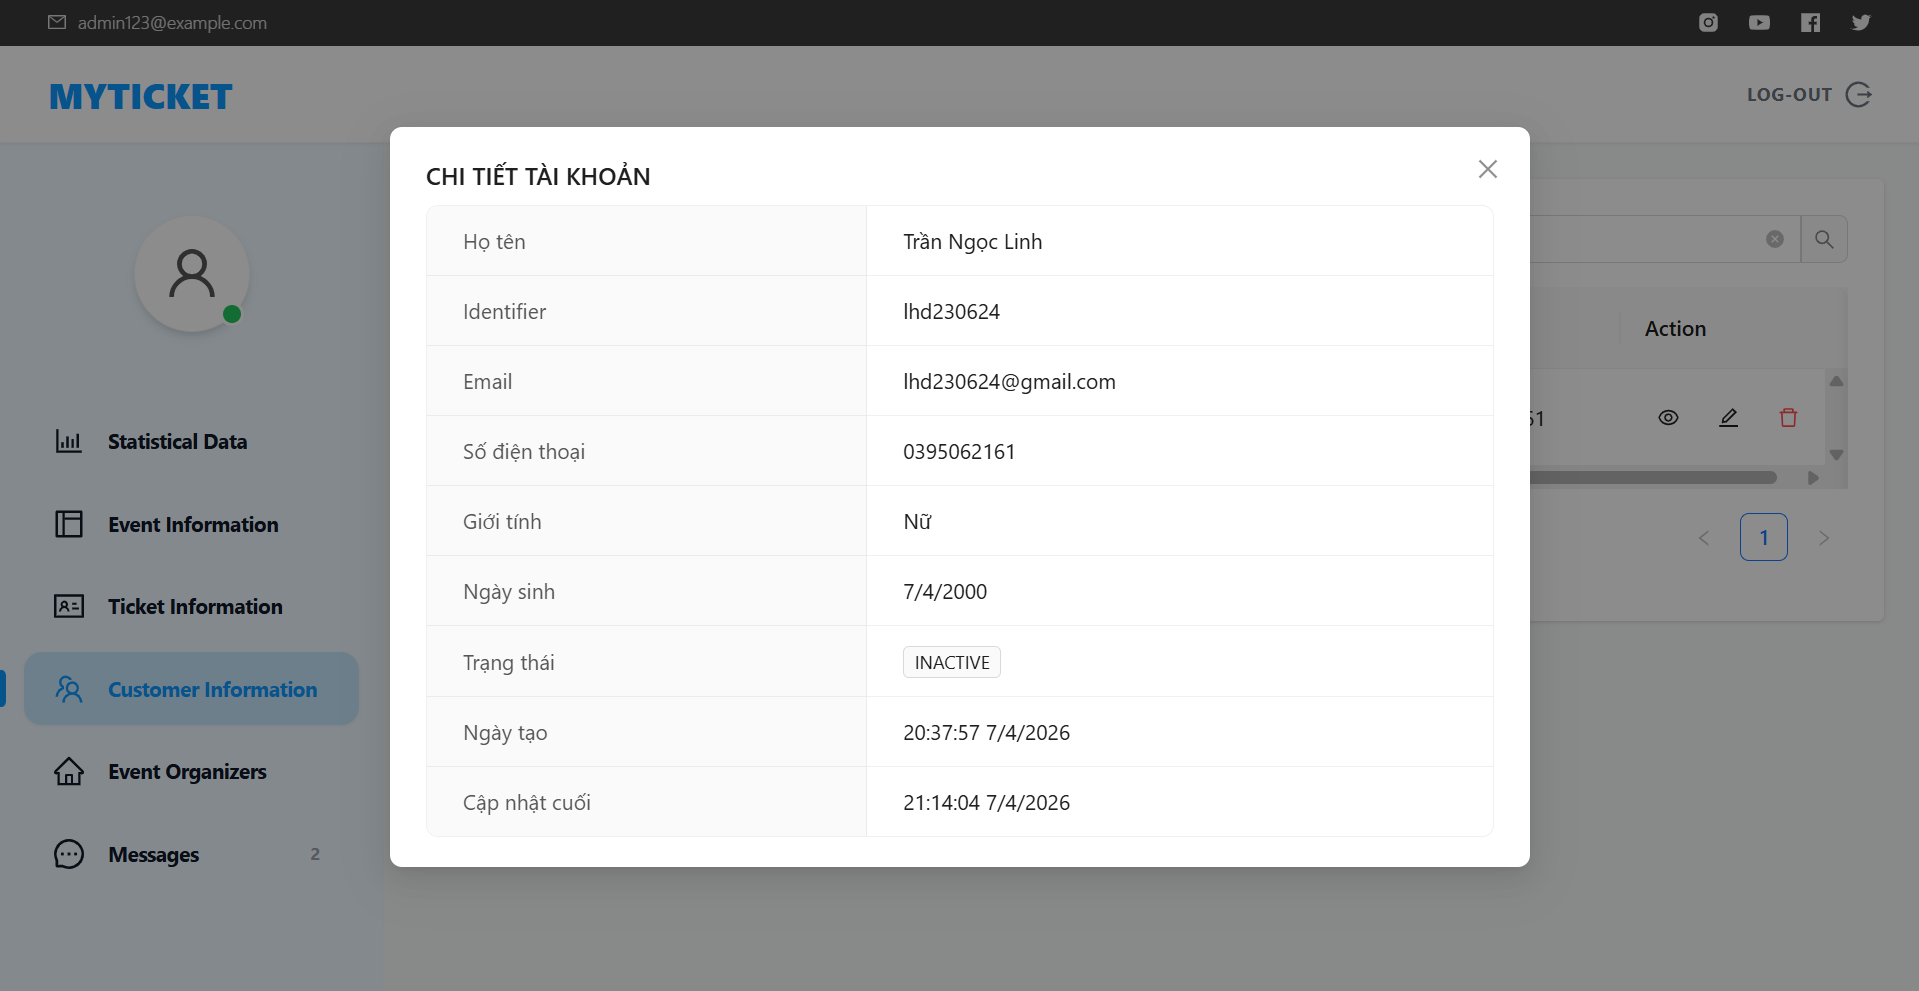
\includegraphics[width=0.65\textwidth]{Contents/UI/QTV/detail info user.png}
        \vspace{15pt}
        \caption{Giao diện hiển thị chi tiết thông tin một người dùng cụ thể tại trang quản lý thông tin người dùng của Quản trị viên}
    \end{figure}
    \item[2.] \textbf{Icon pencil:} Chỉnh sửa thông tin của một người dùng đã chọn.
    \begin{figure}[H]
        \centering
        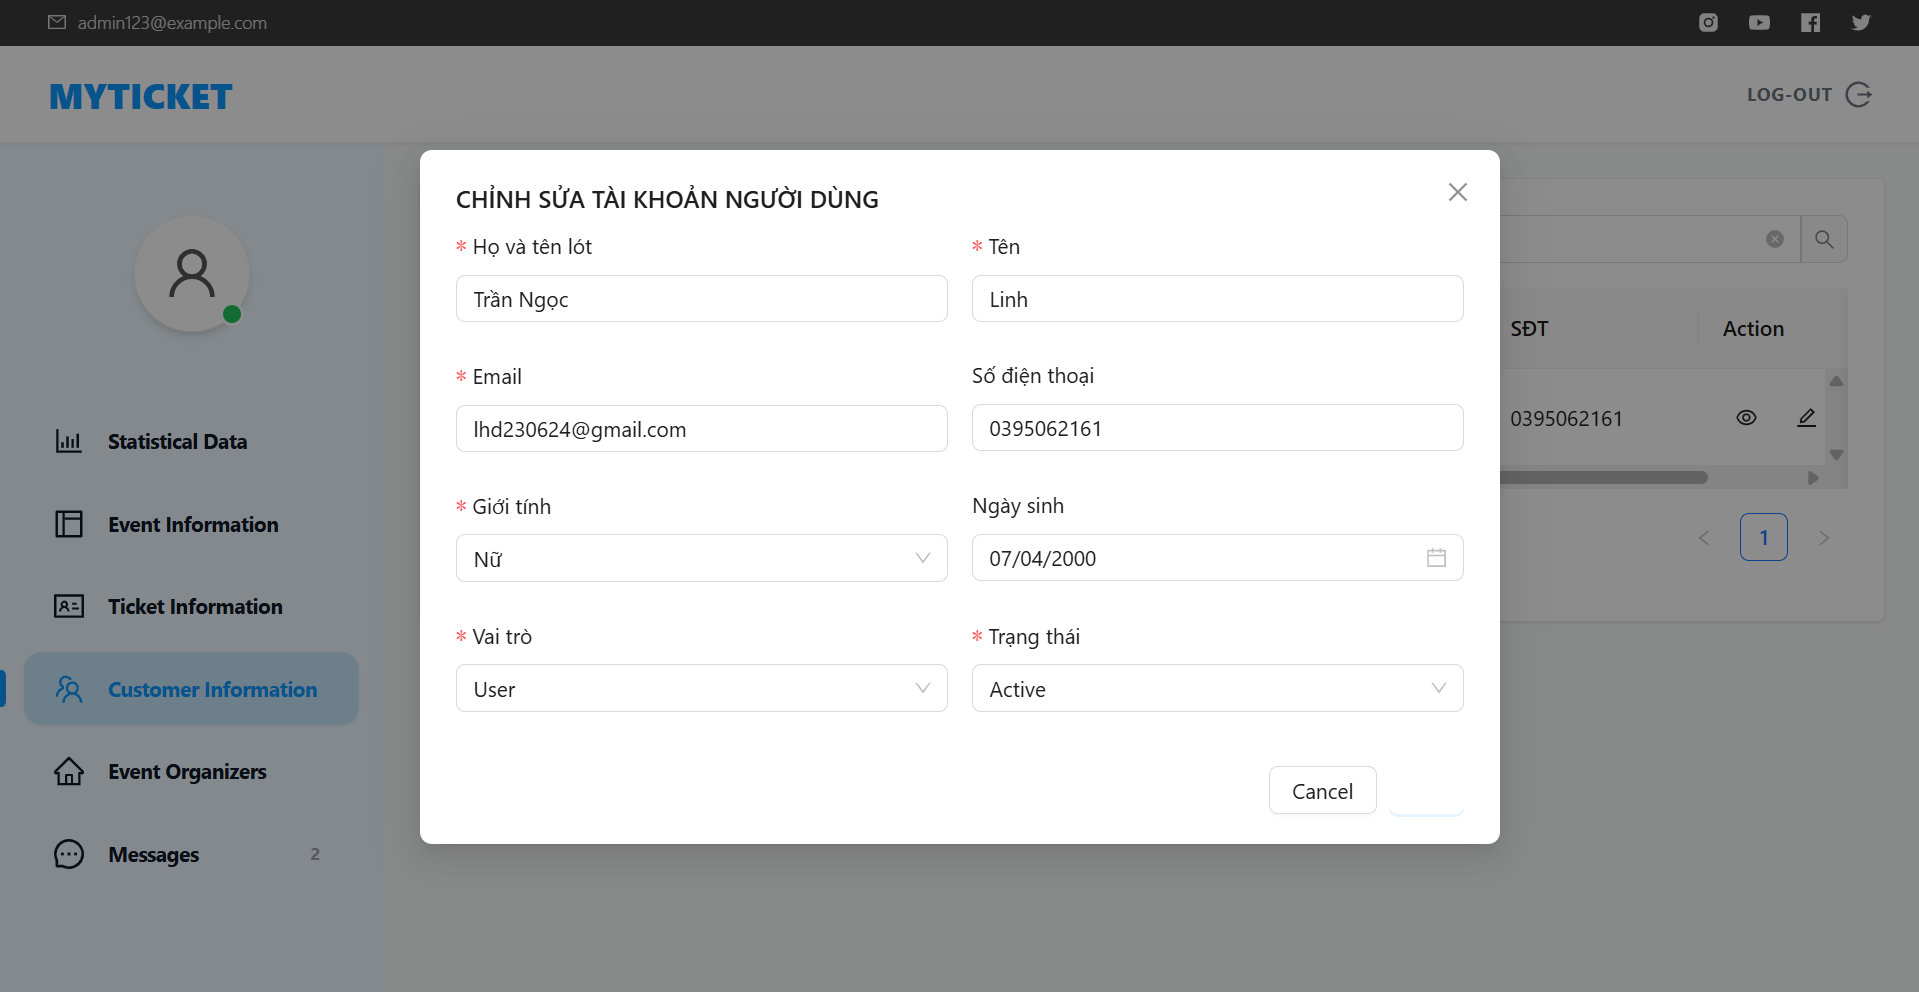
\includegraphics[width=0.65\textwidth]{Contents/UI/QTV/edit user.png}
        \vspace{15pt}
        \caption{Giao diện chỉnh sửa thông tin một người dùng cụ thể tại trang quản lý thông tin người dùng của Quản trị viên}
    \end{figure}
    \item[3.] \textbf{Icon trash:} Xóa một người dùng đã chọn.
    \begin{figure}[H]
        \centering
        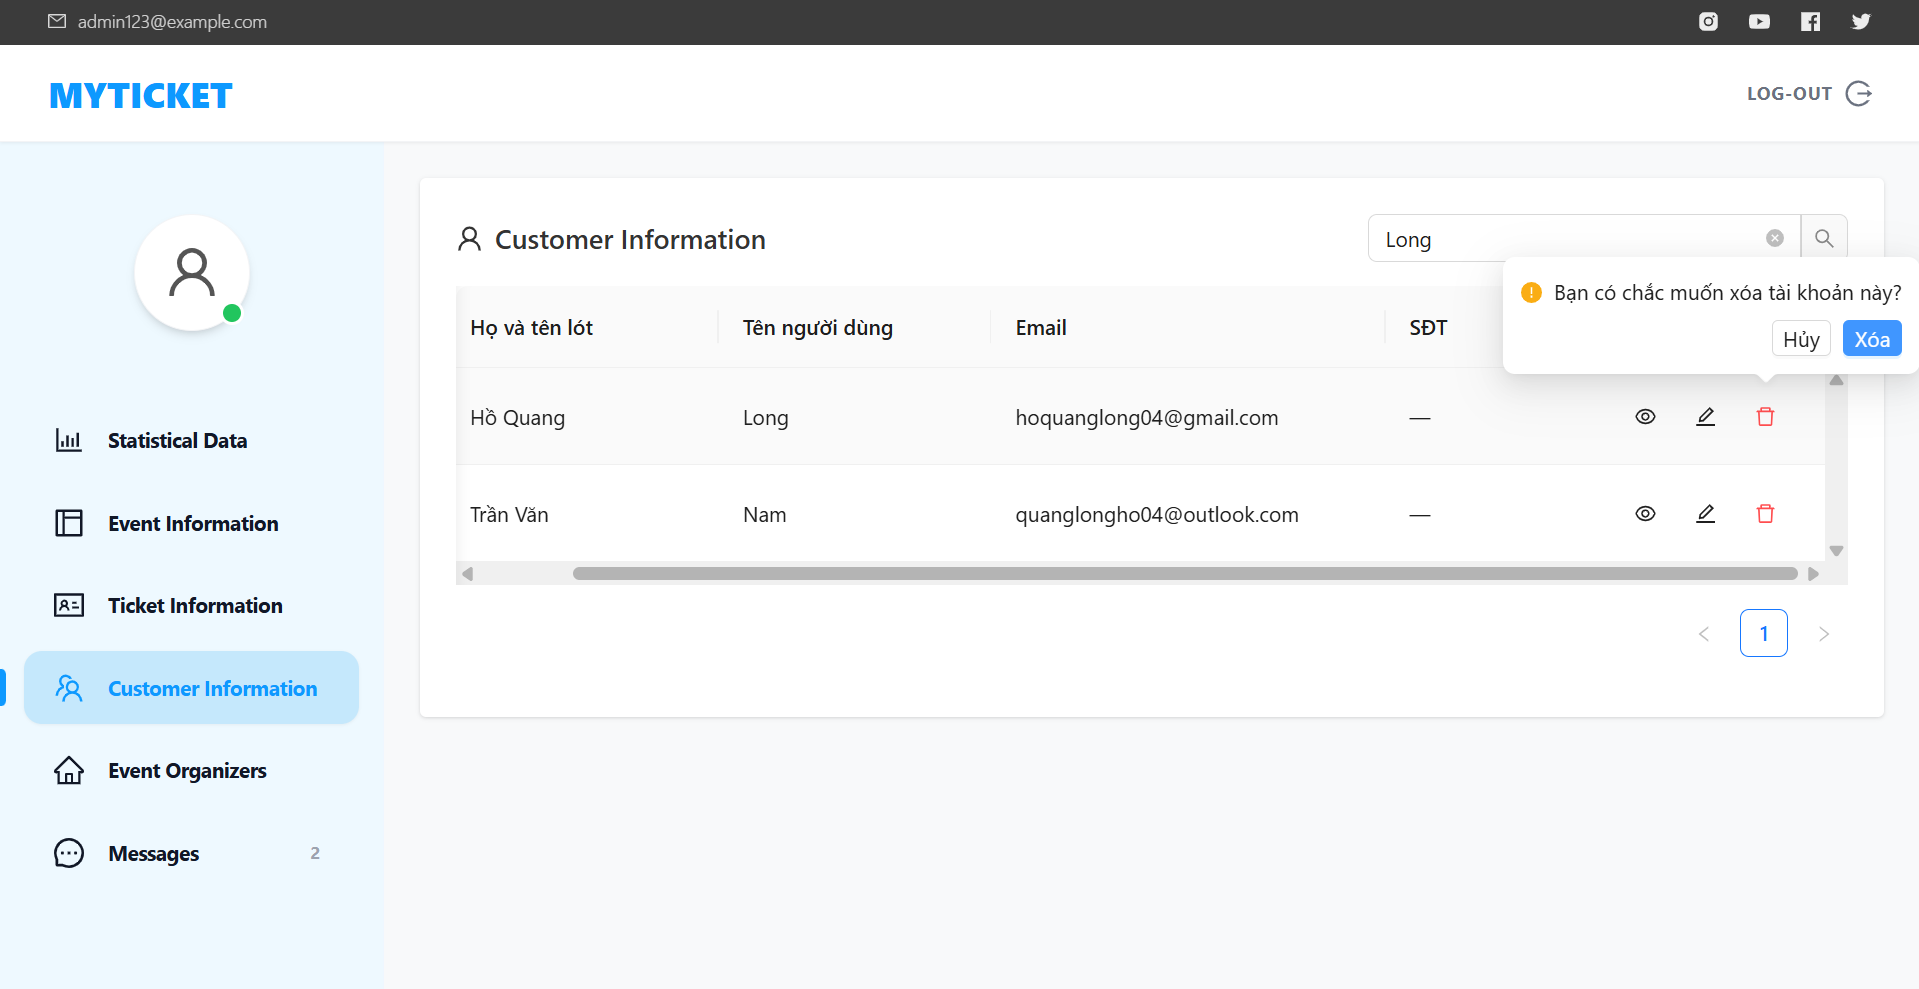
\includegraphics[width=0.65\textwidth]{Contents/UI/QTV/delete user.png}
        \vspace{15pt}
        \caption{Giao diện xác nhận xóa một người dùng cụ thể tại trang quản lý thông tin người dùng của Quản trị viên}
    \end{figure}
\end{itemize}

\subsubsection{Quản lý cài đặt tài khoản}
\begin{figure}[H]
    \centering
    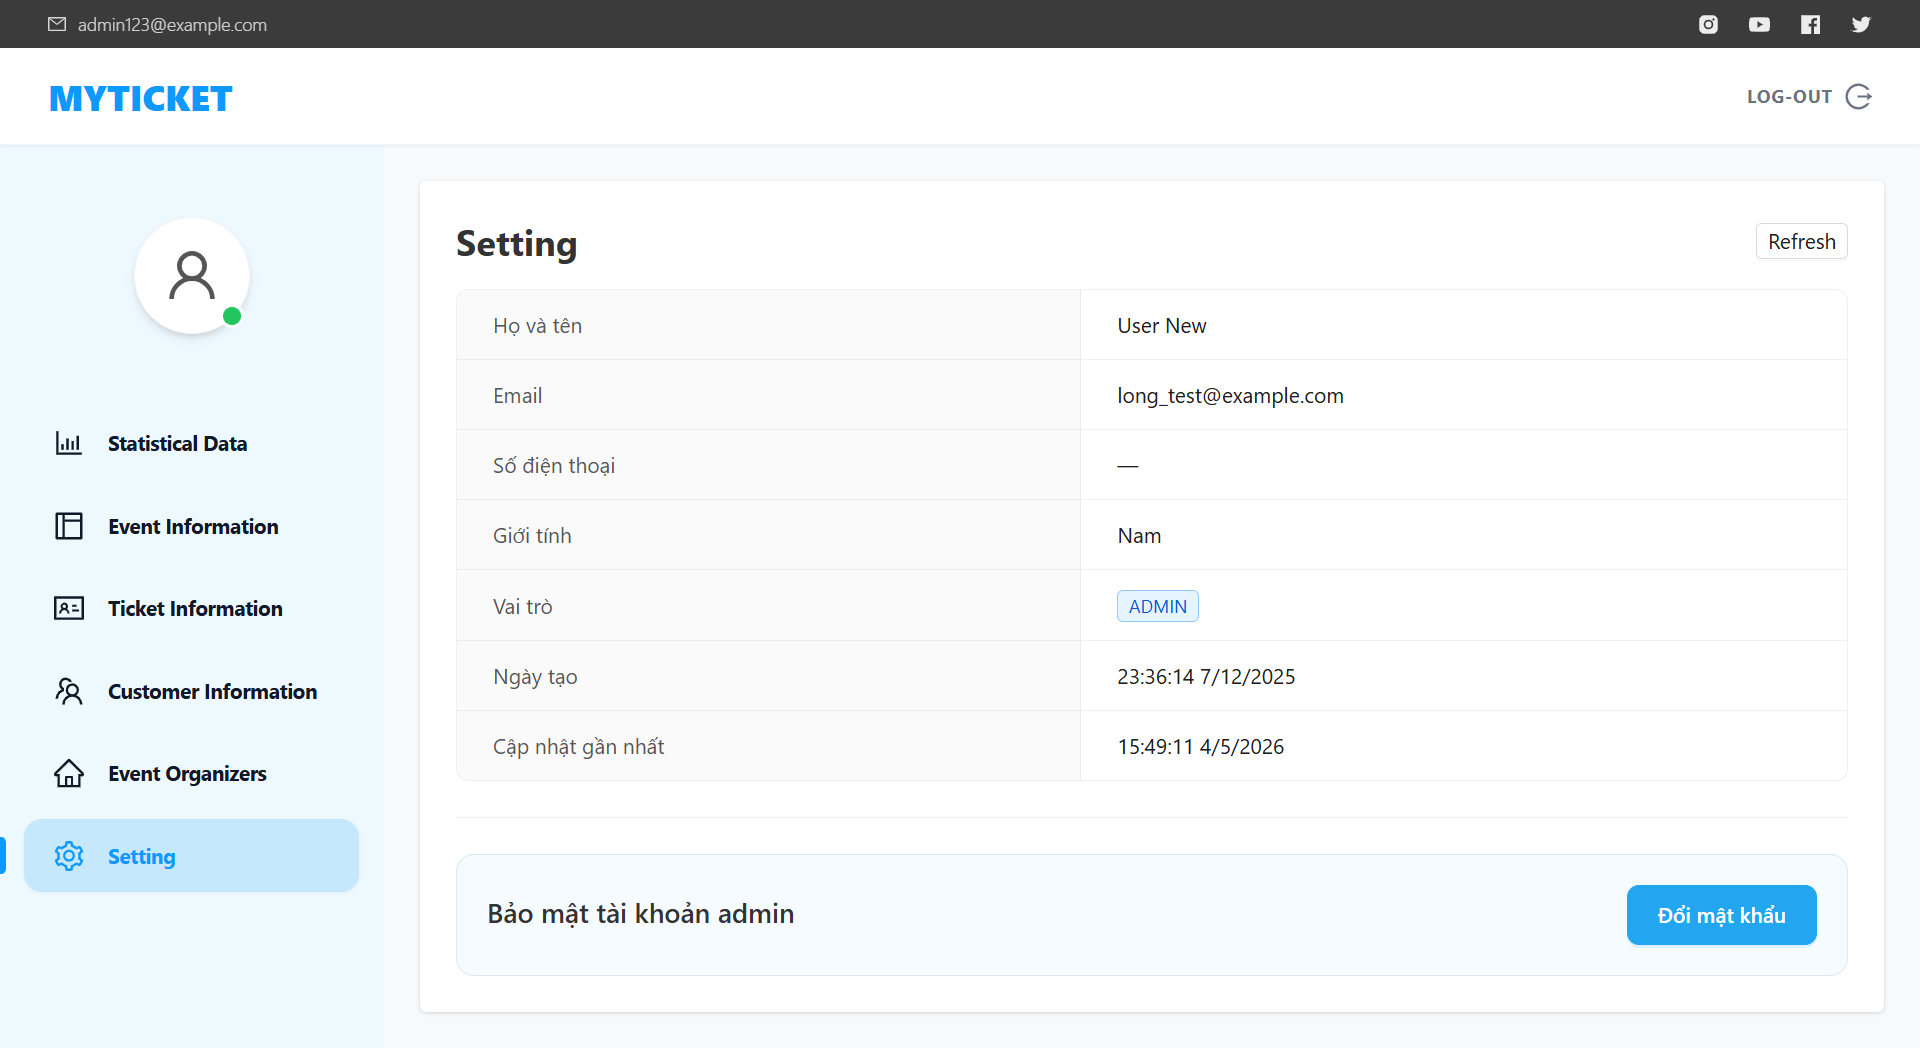
\includegraphics[width=0.65\textwidth]{Contents/UI/QTV/setting.png}
    \vspace{15pt}
    \caption{Giao diện quản lý cài đặt tài khoản của Quản trị viên}
\end{figure}
\indent \indent \textbf{Mô tả:} \\
\indent - Quản trị viên cần nhấn vào mục "Settings" ở thanh navbar để truy cập vào trang này.\\
\indent - Tại đây, Quản trị viên có thể xem thông tin tài khoản của mình như tên, email, số điện thoại, v.v. Quản trị viên có thể nhấn nút "Refresh" để cập nhật lại thông tin cá nhân nếu có sự thay đổi.\\
\indent - Ngoài ra, Quản trị viên cũng có thể nhấn vào nút "Thay đổi mật khẩu" để thay đổi mật khẩu tài khoản của mình. Khi đó, hệ thống sẽ hiển thị một pop up để Quản trị viên điền thông tin mật khẩu cũ, mật khẩu mới và xác nhận mật khẩu mới. Sau khi điền xong thông tin, Quản trị viên cần nhấn nút "Confirm" để hoàn tất việc thay đổi mật khẩu.